% Copyright (c) 2008-2009 solvethis
% Copyright (c) 2010-2016,2018-2019,2021 Casper Ti. Vector
% Copyright (c) 2021 Kurapica
% Copyright (c) 2021 iofu728
% Overleaf version.

%*********************************************************************
% iofu728-pkuthss: 北京大学研究生学位论文模板
% 2021/06/09 v1.0.0
%
% 重要提示:
%   1. 当前overleaf版符合2021研究生学位论文要求,可通过图书馆审核
%   2. 当前版本基于pkuthss v1.9.1
%   3. 请使用UTF-8编码,XeLaTeX方式编译
%   4. 请仔细阅读用户文档
%   5. 修改、使用、发布本文档类请务必遵循LaTeX Project Public License和知识共享4.0
%   6. 如有疑问github/iofu728/pkuthss上提问或联系作者@iofu728
%*********************************************************************

\documentclass[fontset=fandol,ugly]{pkuthss}
  % 学位论文模式  ugly    (默认打开,请保留)
  % 盲审模式      blind   (默认关闭)
  % 字体库        fontset
  %   auto | windows | windows@overleaf | mac | fandol | ubuntu | none
  % windows*, mac为商业字体,如需使用请遵循相应版权协议(默认下overleaf中不可用)
  % fandol与windows效果相近,但字符库偏少,推荐使用(默认);
  % ubuntu字体效果偏差较大; 设为none时需自行配置字体集;

\usepackage[backend=biber,style=gb7714-2015]{biblatex}
  % 参考文献遵循GB/T 7714-2015标准,使用biblatex-gb7714-2015 宏包。
  % 此处使用顺序编码制,如使用著者-出版年制则更改为b7714-2015ay。

% 示例文档用包和设定,该段均可移除.
\usepackage{enumitem,fancyvrb}
\usepackage{extarrows}
\usepackage{cancel}
\usepackage{amsmath}
\usepackage{physics}
\usepackage{booktabs,multirow,longtable,makecell} % 表格相关
\usepackage[perpage]{footmisc}
%\usepackage{perpage}
%\MakePerPage{footnote}
\RecustomVerbatimEnvironment{Verbatim}{Verbatim}{frame = single, tabsize = 4, fontsize=\footnotesize}
\renewcommand{\v}[1]{\boldsymbol{#1}}
\newcommand\pkg[1]{\textsf{#1}}

% 参考文献边距字体
\setlength{\bibitemsep}{3bp}
\renewcommand*{\bibfont}{\zihao{5}\linespread{1.27}\selectfont}

\pkuthssinfo{
	cthesisname = {QFT Notes},
 	thesiscover = {},
	ethesisname = {},
	ctitle = {},
	etitle = {Design and implementation of a XXXXX system based on XXXX},
	cauthor = {}, eauthor = {},
	studentid = {},
	% 具体时间以教务为准,初稿3月,送审4月,答辩5月,最终6月。
	date = {\today},
	school = {},
	cmajor = {}, emajor = {},
	direction = {},
	mentorlines = {0}, % 导师个数
	% 副教授 A.P. 讲师 Lec.
	cmentor = {}, ementor = {},
	ckeywords = {},
	ekeywords = {},
	% 盲审模式参数, 需在documentclass增加blind
	blindid = {XXXXXXXXX}, discipline = {XXXX}
}
\addbibresource{ref.bib}


\begin{document}
	\frontmatter
	\pagestyle{empty}
	\maketitle
	\cleardoublepage
	% 需替换门户版权声明pdf
	%% Copyright (c) 2008-2009 solvethis
% Copyright (c) 2010-2017,2021 Casper Ti. Vector
% Copyright (c) 2021 iofu728
% All rights reserved.
%
% Redistribution and use in source and binary forms, with or without
% modification, are permitted provided that the following conditions are
% met:
%
% * Redistributions of source code must retain the above copyright notice,
%   this list of conditions and the following disclaimer.
% * Redistributions in binary form must reproduce the above copyright
%   notice, this list of conditions and the following disclaimer in the
%   documentation and/or other materials provided with the distribution.
% * Neither the name of Peking University nor the names of its contributors
%   may be used to endorse or promote products derived from this software
%   without specific prior written permission.
%
% THIS SOFTWARE IS PROVIDED BY THE COPYRIGHT HOLDERS AND CONTRIBUTORS "AS
% IS" AND ANY EXPRESS OR IMPLIED WARRANTIES, INCLUDING, BUT NOT LIMITED TO,
% THE IMPLIED WARRANTIES OF MERCHANTABILITY AND FITNESS FOR A PARTICULAR
% PURPOSE ARE DISCLAIMED. IN NO EVENT SHALL THE COPYRIGHT HOLDER OR
% CONTRIBUTORS BE LIABLE FOR ANY DIRECT, INDIRECT, INCIDENTAL, SPECIAL,
% EXEMPLARY, OR CONSEQUENTIAL DAMAGES (INCLUDING, BUT NOT LIMITED TO,
% PROCUREMENT OF SUBSTITUTE GOODS OR SERVICES; LOSS OF USE, DATA, OR
% PROFITS; OR BUSINESS INTERRUPTION) HOWEVER CAUSED AND ON ANY THEORY OF
% LIABILITY, WHETHER IN CONTRACT, STRICT LIABILITY, OR TORT (INCLUDING
% NEGLIGENCE OR OTHERWISE) ARISING IN ANY WAY OUT OF THE USE OF THIS
% SOFTWARE, EVEN IF ADVISED OF THE POSSIBILITY OF SUCH DAMAGE.

% 此处不用 \specialchap,因为学校要求目录不包括其自己及其之前的内容。
\chapter*{版权声明}
% 综合学校的书面要求及 Word 模版来看,版权声明页不用加页眉、页脚。
\thispagestyle{empty}

任何收存和保管本论文各种版本的单位和个人,
未经本论文作者同意,不得将本论文转借他人,
亦不得随意复制、抄录、拍照或以任何方式传播。
否则一旦引起有碍作者著作权之问题,将可能承担法律责任。

% 替换门户下载pdf
\begin{textblock}{1}(-0.8,-0.08)
    \colorbox{white}{
        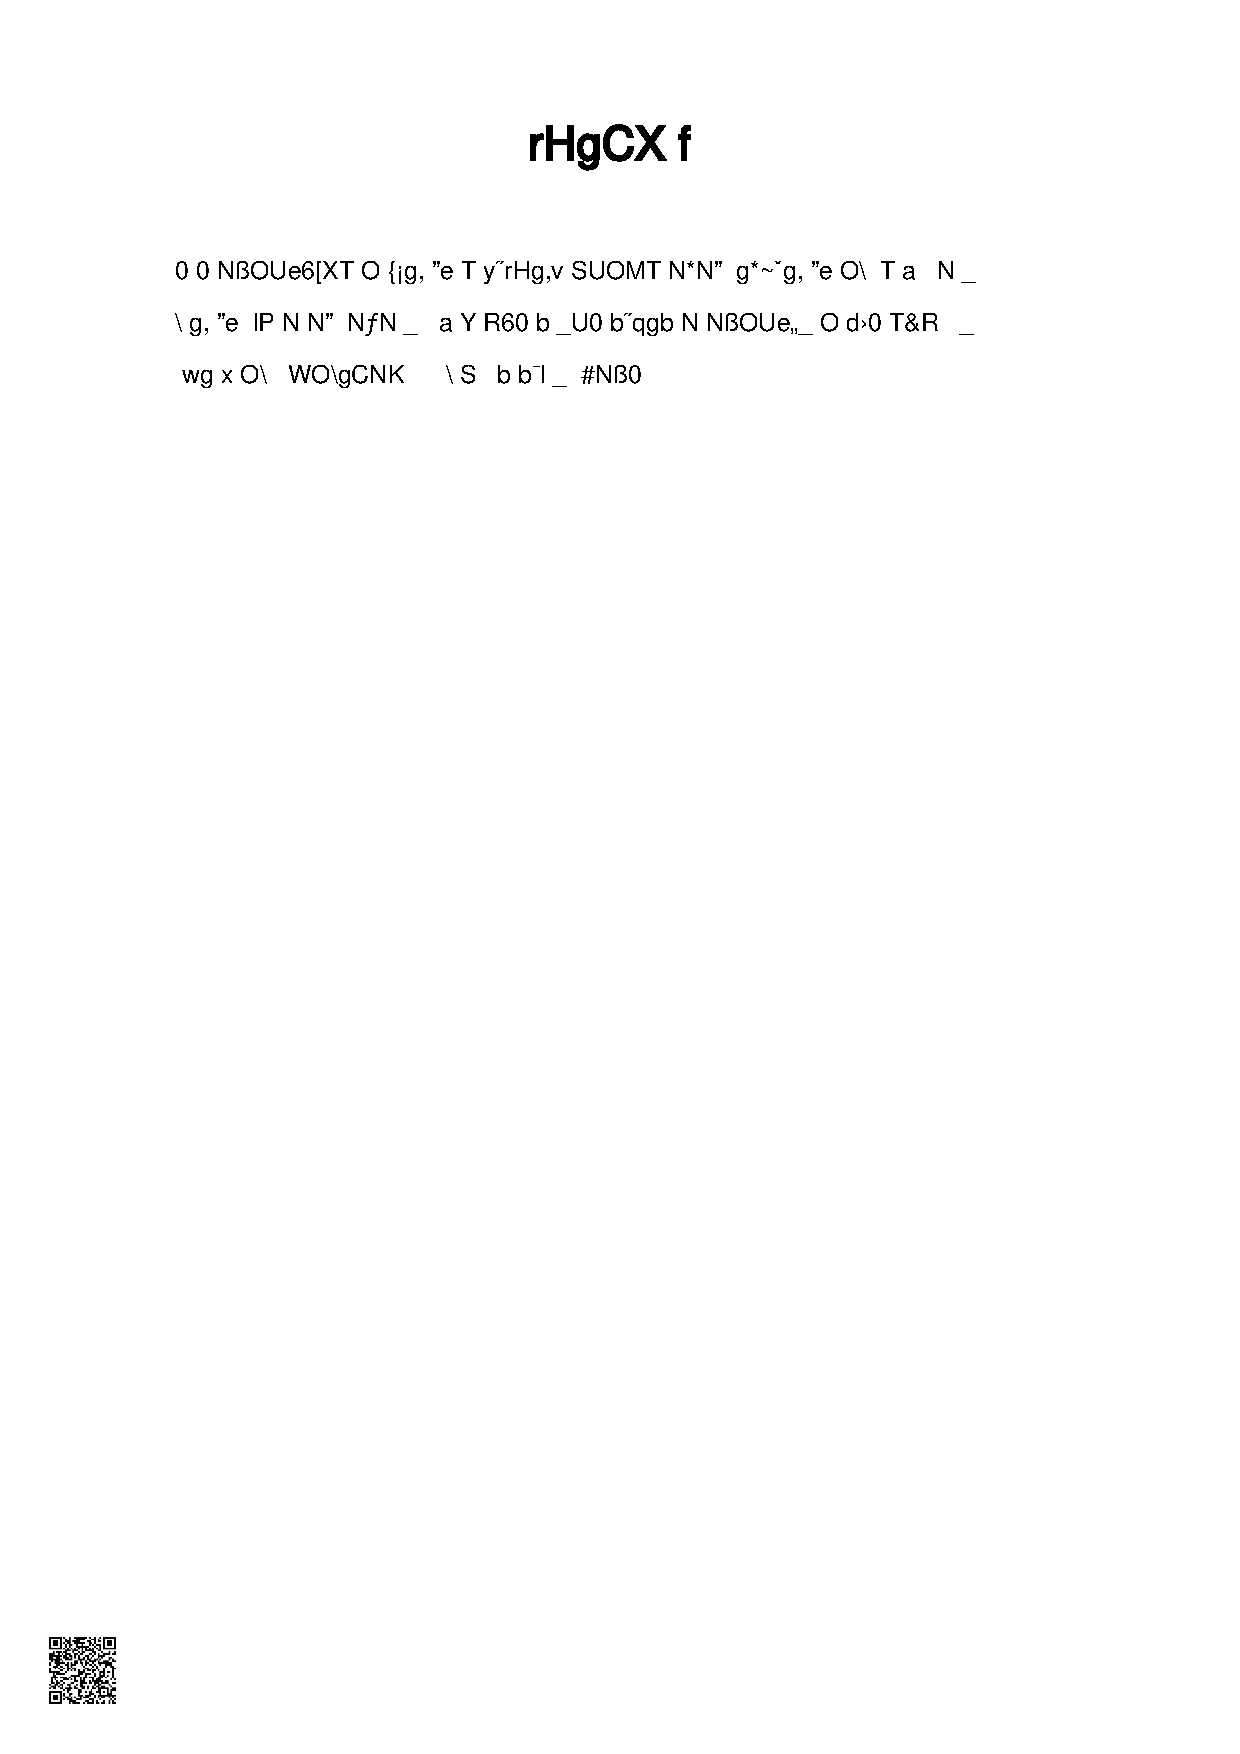
\includegraphics[height = 1.2448\textheight]{img/bqsm_180xxxxxxx.pdf}
    }
\end{textblock}

% vim:ts=4:sw=4

	\cleardoublepage
	\pagestyle{plain}
	\setcounter{page}{0}
	\pagenumbering{Roman}
	\begin{cabstract}
这份notes是根据b站网友上传的贾宇老师2019年在国科大所讲授的量子场论的视频整理而成,由于时间仓促加之本人水平有限,其中必然会存在大量的不足乃至错误之处,如发现问题/错误或有任何建议或者单纯想聊聊天,可以通过以下途径:ddhy@pku.edu.cn
\end{cabstract}



% vim:ts=4:sw=4

	\tableofcontents
	% 如有需要使用主要符号对照表
	%\begin{denotation}

\item[$x,y,m,n,t$] 标量,通常为变量
\item[$K,L,D,M,N,T$] 标量,通常为超参数
\item[$x\in \mathbb{R}^{D}$] D维列向量
\item[$(x_1,\cdots,x_D)$] D维行向量
\item[$(x_1,\cdots,x_D)^T$ or $(x_1;\cdots;x_D)^T$]  D维行向量
\item[$\v A\in \mathbb{R}^{K\times D}$]  大小为$K\times D$的矩阵
\item[$x\in \mathbb{R}^{KD}$]  ($KD$)维的向量
\item[$\mathbb{M}_i$ or $\mathbb{M}_i(\v x)$]  第$i$列为$\v 1$(或者$\v x$),其余为$\v 0$的矩阵
\item[$diag(\v x)$]  对角矩阵,其对角元素为$\v x$
\item[$\v I_N$ or $I$]  ($N\times N$)的单位阵
\item[$diag(\v A)$]  列向量,其元素为$\v A$的对角元素
\item[$\v A \in \mathbb{R}^{D_1\times D_2\times \cdots \times D_K}$]  大小为$D_1\times D_2\times \cdots \times D_K$的张量
\item[$\{x^{(n)}\}^{N}_{n=1}$]  集合
\item[$\{(x^{(n)},y^{(n)})\}^{N}_{n=1}$]  数据集
\item[$\mathcal{N}(\v x;\mu,\sum)$]  变量$x$服从均值为$\mu$,方差为$\sum$的高斯分布

\end{denotation}

\footnotetext[1]{本符号对照表内容选自\citeauthor{qiu2020nndl}老师的《神经网络与深度学习》\cite{qiu2020nndl}一书。}

	\mainmatter
	\chapter{什么是QFT?}
\section{为什么要学习量子场论}
量子场论包含无穷多自由度,比单粒子非相对论要复杂很多。在非相对论情况,我们比较熟悉的是谐振子的情况:$H=\frac{\textbf{p}^{2}}{2m}+\frac{1}{2}m^{2}\omega^{2}x^{2}$,
其能级为$E_{n}=(n+\frac{1}{2})\hbar\omega$,n=1,2,3 $\cdots$。
量子场论可以看成是无穷多个谐振子的联合,因此即使我们对于单粒子的谐振子情况已经了解得比较透彻了,但是在场论里面对无穷多谐振子耦合在一起的情况,仍然需要面对极其困难的复杂性。

量子场论之所以重要是因为其具有极其广泛的应用,可以应用在物理学的很多分支当中。尽管其发源于高能物理,但如今在高能物理、核物理、原子物理、凝聚态物理、宇宙学等方面仍有重要的作用,从最微观到最宏观都有发挥其作用的空间。本课程主要关注量子场论在高能物理中的应用。

量子场论具有非常强大的预言能力。电子的反常磁矩是人类在自然科学中理论和实验吻合得最好的例子之一,QED的预言与实验测量到小数点后第九位数字仍然是一致的。

20世纪初发展起来的狭义相对论和量子力学可以看作是牛顿体系在两个不同纬度的推广,前者成功描述了运动速度可以与光速相比的系统,后者成功描述了角动量与普朗克常数可以相比的微观系统,但这两大理论内部是不自洽的,为了能够使狭义相对论($E=m c^{2}$)与量子力学($i \hbar \frac{\partial}{\partial t}\psi=\hat{H}\psi$)统一起来,早期人们进行过许多尝试,但结果是人们经过多年的努力后发现,简单的把薛定谔方程改成协变的形式会遇到各种问题,唯一自洽的可能是抛弃固定粒子数的概念,引入量子场论的框架。
\begin{center}
QFT=SQ+QM
\end{center}

为什么学习粒子物理需要学习场论?两者之间有什么关系?Faraday提出了场的概念,Einstein提出了光量子的概念。可以认为,粒子是场激发对应的量子,即粒子首先是一个量子。考虑一个池塘,其中的水面是静止的,往池塘里扔进一个石子扰动水面,会在水面上出现涟漪,如果我们认为水是场,那么水波就是场激发产生的粒子。类似地,光子可以认为是电磁场激发后,具有确定能量和动量的水波,它具有粒子的属性。今后我们将使用这种图像理解许多粒子,如Higgs粒子,它可以通过激发一个标量场得到,电子则可以通过激发连续分布的电子场得到。

量子场论可以用来描述粒子数改变的过程。非相对论量子力学中粒子数是严格守恒的,但在真实的世界中有很多复杂的现象,难以使用量子力学来描述,在高能物理中,粒子能量较高,可以衰变成其他粒子,而在低能的情况,如凝聚态物理中,其能量小于电子的静止能量,因而无法产生新的电子,这里我们主要关注相对论性的量子场论。
以下考虑两个例子。

第一个例子是原子的自发辐射。考虑一个处于第一激发态的粒子,它有一定的几率会回到基态,假设第一激发态与基态的能量差是$\Delta E$,由于能量守恒,这一过程会释放出一个能量为$\Delta E$的光子$\gamma$,即$e^{-} \longrightarrow e^{-}+\gamma$。这一过程是一个粒子数改变的过程,其初态只有一个电子,而末态则有一个电子和一个光子。量子力学无法解释这一个光子从何而来,从场论的角度,光子可以认为是电磁场的激发态对应的量子,由于电磁场与电子场进行相互作用,从而有一定的几率电子场可以把电磁场激发出一个光子。

第二个例子是原子核的$\beta$衰变。这是一个由弱相互作用引导的过程:$n \longrightarrow p+e^{-}+\overline{\nu}_{e}$,其中涉及到了四种不同的粒子产生和湮灭的过程。历史上,1930sFeimi引入了4粒子相互作用来解释这一现象。
\section{历史回顾——相对论性量子力学}
描写固定粒子数的相对论性粒子的相对论性量子力学始于de Broglie、Schr$\ddot{\rm{o}}$dinger、Klein、Gordon、Dirac等人。这一理论在早期获得了一定的成功,但最终遇到了三个困难,必须让位于量子场论。这三个困难是:
\begin{itemize}
    \item 负能解问题,会导致不存在稳定的真空
    \item 负几率问题,统计诠释中$\rho=|\psi(x)|^{2}$代表粒子出现在某点的几率,其必须正定,但是在相对论性量子力学中这一正定性不再成立,意味着我们必须放弃波函数的几率诠释
    \item 因果性破坏
\end{itemize}

下面我们来谈论一些具体的历史。
Einstein光量子假设(1905):光子能量是一份一份的,$E=h\nu=\hbar \omega$,$\nu$是频率,$\omega$是角频率。

de Broglie物质波假设(1923):受狭义相对论以及光量子假设的启发,考虑一个自由电子,其四动量为$p^{\mu}=(\frac{{E}}{c},\vec{p})$,对应的物质波的波函数为平面波形式\footnote{这里采用的度规为$g^{\mu\nu}=diag(-1,1,1,1)$,今后如不特殊说明我们采用$g^{\mu\nu}=diag(1,-1,-1,-1)$}\footnote{今后所有的四矢量均用不带箭头的量表示,三分量矢量用带箭头的量表示}
\begin{equation}
    e^{ikx}=e^{ik^{\mu}x_{\mu}}e^{i\vec{k}\cdot \vec{x}-i \omega t}
\end{equation}
其中$k^{\mu}=(\frac{\omega}{c},\vec{k})$,$x^{\mu}=(ct,\vec{x})$,为了使得相位是Lorentz不变量,我们必须有$k^{\mu}$是四矢量。对于自由粒子的简单情况,电子自身的四动量$p^{\mu}$与$k^{\mu}$不应当是独立的,它们之间应该存在一定的比例关系,$k^{\mu}\propto p^{\mu}$。根据光量子假设,我们有$E=\hbar \omega$,因此$p^{\mu}=\hbar k^{\mu}$,写成分量的形式有$E=\hbar \omega,\vec{p}=\hbar \vec{k}=\frac{h}{\lambda}$。
对于一个物质粒子,它对应的物质波的粒子属性是由粒子的四动量$p$刻画的,波的属性是由波矢$k$刻画的,上面的结果告诉我们这两个量相差一个比例系数$\hbar$,这是进入量子世界的桥梁。
由于实在的电子要满足在壳条件$p^{2}=p^{\mu}p_{\mu}=m^{2}c^{2}$,其中$m$为电子的静止质量,是一个Lorentz不变量。
这样我们得到了相对性电子的质能关系为
\begin{equation}
    \label{zhineng}
    E^{2}=\vec{p}^{2}c^{2}+m^{2}c^{4}
\end{equation}
由于$p^{\mu}=\hbar k^{\mu}$,对于波矢而言我们有
\begin{equation}
    \label{2}
    \frac{\omega^{2}}{c^{2}}=\vec{k}^{2}+ \left( \frac{mc}{\hbar} \right)^{2}
\end{equation}
即$\omega$和$k^{\mu}$也不是独立的。Davisson$\&$Germer(1927)通过观察到电子散射晶体的衍射现象,证实了de Broglie的物质波假设。
\subsection{Klein-Gordon方程}
这一方程最早是由Schr$\ddot{\rm{o}}$dinger得出,是最简单的相对论性的波动方程。
下面我们采用类比的方法来得到这一方程。首先回顾一下Schr$\ddot{\rm{o}}$dinger方程的推导\footnote{这里老师的表达似不太严谨,Schr$\ddot{\rm{o}}$dinger方程并非基于某一更底层的假设推导而来,事实上这一方程自身是作为一项基本假设写入了非相对论性量子力学之中}。考虑一个非相对论自由粒子,其质能关系(或称色散关系)为$E=\frac{\vec{p}^{2}}{2m}$,考虑正则量子化框架,在其中做替换$E=\hbar \omega \rightarrow \hbar i \frac{\partial}{\partial t}, \vec{p}=\hbar\vec{k} \rightarrow \hbar (-i \nabla)$,得到(作用到一个波函数$\psi(x)$之后)
\begin{equation}
i\hbar\frac{\partial}{\partial t}\psi(x)=-\frac{\hbar^{2}\nabla^{2}}{2m}\psi(x)
\end{equation}
这就是Schr$\ddot{\rm{o}}$dinger方程。

接下来我们在相对论下的质能关系(\ref{zhineng})中做同样的替换,并作用到波函数上,得到
\begin{equation}
\label{KGpre}
\left[-\hbar^{2}\frac{\partial^{2}}{\partial^{2} t}+\hbar^{2}c^{2}\nabla^{2}-m^2c^{4}\right]\psi(\vec{x},t)=0
\end{equation}
我们定义达朗贝尔算符$\Box=\partial^{2}=g^{\mu\nu}\partial_{\mu}\partial_{\nu}=\frac{1}{c^{2}}\frac{\partial^{2}}{\partial^{2} t}-\nabla^{2}$,这一算符是Lorentz不变的。利用这一算符重写(\ref{KGpre})我们可以得到
\begin{equation}
    \label{KG}
      \left[\partial^{2}+\left(\frac{mc}{\hbar}\right)^{2}\right]\psi(\vec{x},t)=0
\end{equation}
此即为Klein-Gordon方程。
这是一个相对论性的波动方程,$\psi(x)$为波函数,将来在学习经典场论时我们将重新遇到这个方程,并将赋予其完全不同的物理诠释。

下面讨论其平面波解。令$\psi(x)=e^{\frac{i}{\hbar}(\vec{p}\cdot \vec{x}-Et)}$,将其带入(\ref{KG}),可以得到
\begin{equation}
     E^{2}=p^{2}c^{2}+m^{2}c^{4}
\end{equation}
从而得到
\begin{equation}
    E=\pm \sqrt{p^{2}c^{2}+m^{2}c^{4}}
\end{equation}
我们得到了一个负能解。在经典的狭义相对论中我们也会遇到负能解,但这不会导致任何严重的后果,这是因为在经典的世界里能量是连续变化的,一个初始状态能量为正($E>0$)的粒子,不可能连续的变成能量为$-E$的粒子,但是在量子力学中,由于量子跃迁的存在,处于正能态$E$的粒子可以以一定几率跃迁到负能态$-E$,同时辐射出一个高能光子,这一过程并没有被对称性所禁戒。这说明如果我们有一系列初始的处于正能态的粒子,它们会不断向负能态跃迁,且能量越高,其对应的负能态粒子能量越低,这将导致能量没有下界,从而没有稳定的基态,导致真空不稳定。正如我们之前提到过的,这是一个很严重的问题。

下面来讨论K-G方程中的负几率问题。在非相对论的情况下,考虑单粒子的情况,其Hamiltonian为$H=\frac{\vec{p}^{2}}{2m}+V(\vec{x})$,从Schr$\ddot{\rm{o}}$dinger方程出发,我们可以得到连续性方程
\begin{equation}
    \frac{\partial}{\partial t}|\psi|^{2}-\nabla \cdot \left[\frac{i\hbar}{2m}\left(\psi^{*}\nabla\psi-\psi \nabla\psi^{*}\right)\right]=0
\end{equation}
其中我们称$\rho(x)=|\psi(x)|^{2}$为几率密度,$\vec{j}(x)=-\left[\frac{i\hbar}{2m}\left(\psi^{*}\nabla\psi-\psi \nabla\psi^{*}\right)\right]$为几率流,从而我们可以把连续性方程改写为
\begin{equation}
\label{jilv}
    \frac{\partial \rho(x)}{\partial t}+\nabla \cdot \vec{j}{x}=0
\end{equation}
定义几率密度的全空间积分为$Q(t)=\int d^{3}x\rho(x)$,
并对(\ref{jilv})两边做全空间积分,有
\begin{equation}
    \frac{dQ(t)}{dt}=\int d^{3}x \frac{\partial \rho(t,\vec{x})}{\partial t}=-\int d^{3}x \nabla \cdot \vec{j}(t,\vec{x})=-\int_{S}\vec{j}\cdot \vec{d\Sigma}
\end{equation}
其中最后一个等号用到了Gauss公式,如果认为$\vec{j}$在$|\vec{x}|\rightarrow \infty$时足够快地趋于0,当S为一半径趋于$\infty$的球面时,我们就得到
\begin{equation}
    \frac{dQ(t)}{dt}=0
\end{equation}
于是我们得到$Q(t)$是守恒量,也称为守恒荷。这一点在物理上是清楚的,根据概率诠释,粒子在全空间出现的总概率应该满足$\int |\psi(x)|^{2}=1$(对$\psi$归一化后),从而$Q(t)$显然应该是不随时间变化的。
在上面的推导中,我们由定义可以看出$\rho(x)=|\psi(x)|^{2}$是正定的。

对于K-G方程,我们根据与上面相同的方法,我们可以导出连续性方程(\ref{jilv})的形式,但是与非相对论量子力学不同的是,在这里我们有
\begin{equation}
\left\{
        \begin{array}{ll}
            \rho(x)=N Im \left[\psi^{*}\frac{\partial}{\partial t}\psi\right] \\
            \vec{j}(x)=Nc^{2}Im \left[\psi^{*}\nabla \psi\right]
        \end{array}
    \right.
\end{equation}
其中$N$是任一待定常数,$c$为光速。
此时$rho(x)$不再是一个正定的量,这是因为K-G方程中包含时间的二阶导数。
\begin{center}
   \textbf{Digression} 
\end{center}

考虑到$E=\frac{\vec{p}^{2}}{2m}$是$E^{2}=p^{2}c^{2}+m^{2}c^{4}$的非相对论极限,因此从K-G方程出发,通过非相对论近似,我们应当可以得到Schr$\ddot{\rm{o}}$dinger方程,下面来验证这一点。

为方便,我们做拟设(ansatz),将波函数的时间依赖关系分为包含静止质量$m_{0}$的部分与其他部分
\begin{equation}
\label{ansatz}
    \psi(\vec{x},t)=\phi(\vec{x},t)e^{-\frac{i}{\hbar}m_{0}c^{2}t}
\end{equation}
在非相对论情况下,$E'=E-m_{0}c^{2}$是一个小量,满足$E' \ll m_{0}c^{2}$,因此我们有
\begin{equation}
    \left|i\hbar \frac{\partial \phi}{\partial t}\right| \approx E'\phi \ll m_{0}c^{2}\phi
\end{equation}
将(\ref{ansatz})对时间求导数可得
\begin{equation}
    \frac{\partial^{2} \psi}{\partial t^{2}}=\left( \frac{\partial^{2} \phi}{\partial t^{2}}-\frac{2i m_{0}c^{2}}{\hbar}\frac{\partial \phi}{\partial t} -\frac{m_{0}^{2}c^{4}}{\hbar^{2}}\phi\right)e^{-\frac{i}{\hbar}m_{0}c^{2}t}\approx -\left( \frac{2i m_{0}c^{2}}{\hbar}\frac{\partial \phi}{\partial t} +\frac{m_{0}^{2}c^{4}}{\hbar^{2}}\phi\right)e^{-\frac{i}{\hbar}m_{0}c^{2}t}
\end{equation}
将之带入(\ref{KGpre})可得,
\begin{equation}
-\frac{1}{c^{2}}\left[ \frac{2i m_{0}c^{2}}{\hbar}\frac{\partial \phi}{\partial t} +\frac{m_{0}^{2}c^{4}}{\hbar^{2}}\phi\right]e^{-\frac{i}{\hbar}m_{0}c^{2}t}=(\nabla^{2}-\frac{m_{0}^{2}c^{2}}{\hbar^{2}})\phi
\end{equation}
整理可得
\begin{equation}
\label{schro}
    i\hbar\frac{\partial\phi}{\partial t}=-\frac{\hbar^{2}}{2m_{0}}\nabla^{2}\phi
\end{equation}
此即为Schr$\ddot{\rm{o}}$dinger方程。

粒子是由波动方程来描述的,其属性不应该与相对论或非相对论情形有关,因此,由于Schr$\ddot{\rm{o}}$dinger方程(\ref{schro})描述的是自由无自旋粒子,我们可以推断K-G方程也同样描述了无自旋粒子。



\subsection{Dirac 方程}
Dirac试图给出一个自洽的相对论性的波动方程,这里自洽的内涵主要是指要克服负几率问题,事实上我们将会看到,Dirac提出的方案在一定程度上也解决了负能解的问题,这导致他与Schr$\ddot{\rm{o}}$dinger一起分享了1933年的诺贝尔物理学奖。

在上一节中我们看到,导致负几率问题的一个主要原因是在K-G方程中含有对时间的二阶导数,Dirac为了克服这一问题,坚持只包含时间一阶导数的构造方式,考虑到时间与空间地位的等同性,其构造的方程中也应该只出现空间的一阶导数项,同时为了避免根号下出现Nabla算符,Dirac把波函数$\psi$扩展成一个列矢量$\vec{\psi}=(\psi_{1},\psi_{2},\cdots,\psi_{n})^{\top}$,称之为旋量(spinor),从而Hamiltonian成为一个$n\times n$的矩阵
\begin{equation}
\label{Dirac}
    i\hbar \frac{\partial}{\partial t}\psi=H\psi=\left[-i\hbar c \vec{\pmb{\alpha}}\cdot \nabla +\pmb{\beta}m_{0}c^{2}\right]\psi
\end{equation}
其中$\vec{\pmb{\alpha}}=(\pmb{\alpha}_{1},\pmb{\alpha}_{2},\pmb{\alpha}_{3})$,$\pmb{\alpha}_{i}(i=1,2,3)$与$\pmb{\beta}$均为待定的$n\times n$矩阵,为方便,今后省略掉$\vec{\psi}$上的箭头,因为波函数的形式根据上下文是明显的。
接下来我们来确定$H$中不确定的参量。

如果$\psi$满足Schr$\ddot{\rm{o}}$dinger方程,我们应当期望有
\begin{equation}
\label{dir}
\left(i\hbar \frac{\partial}{\partial t}\right)^{2}\psi=H^{2}\psi
\end{equation}
我们知道对于时间依赖为二次导数的相对论性波动方程为K-G方程,所以我们期望(\ref{dir})回到K-G方程。
展开(\ref{dir})并考虑矩阵乘法的不可对易性,我们可以得到\footnote{这里我们采用了Einstein求和约定,今后如不特殊说明,均默认采用此约定}
\begin{equation}
    -\hbar^{2}\frac{\partial^{2}}{\partial^{2} t}\psi=-\hbar^{2}c^{2}\frac{1}{2}\left\{\pmb{\alpha}^{i},\pmb{\alpha}^{j}\right\}\partial_{i}\partial_{j}\psi-i\hbar m_{0}c^{3}\left\{\pmb{\alpha}^{i},\pmb{\beta}\right\}\partial_{i}\psi+m^{2}_{0}c^{4}\pmb{\beta}^{2}\psi \quad (i,j=1,2,3)
\end{equation}
其中$\left\{A,B\right\}=AB+BA$为反对易关系,今后我们还将遇到对易关系$\left[A,B\right]=AB-BA$,这是在量子力学中就早已经熟知的。

将上式与K-G方程
\begin{equation}
-\hbar^{2}\frac{\partial^{2}}{\partial^{2} t}\psi=-\hbar^{2}c^{2}\nabla^{2}\psi+m^2_{0}c^{4}\psi=0
\end{equation}
对比我们可以得知
\begin{equation}
\label{requsetofDirac}
\left\{
        \begin{array}{lll}
            \left\{\pmb{\alpha}^{i},\pmb{\beta}\right\}=0,i=1,2,3 \\
            \pmb{\beta}^{2}=\pmb{I}  \\
            \left\{\pmb{\alpha}^{i},\pmb{\alpha}^{j}\right\}=2\delta^{ij}\pmb{I}, i,j=1,2,3
        \end{array}
    \right.
\end{equation}
其中$\delta^{ij}$为Kronecker symbol,$\pmb{I}$为$n\times n$单位阵。
特别地,在$\left\{\pmb{\alpha}^{i},\pmb{\alpha}^{j}\right\}$中取$i=j$,我们可以得到$2(\pmb{\alpha}^{i})^{2}=2\pmb{I}$,即$(\pmb{\alpha}^{i})^{2}=\pmb{I}$(i=1,2,3)。

当$n=2$时,可以证明不存在满足上述所有条件的矩阵\footnote{见本章末尾附录}。事实上,容易验证,当$n=4$时存在一组满足上面所有要求的解,一组可能的解是
\begin{equation}
\label{diracmatrix1}
    \pmb{\alpha}_{i}=\left(                 
  \begin{array}{cc}   
    0 & \pmb{\sigma}_{i}  \\  
    \pmb{\sigma_{i}} & 0 \\  
  \end{array}
\right),\quad
\pmb{\beta}=\left(                 
  \begin{array}{cc}   
    \pmb{I}_{2} & 0  \\  
    0 & -\pmb{I}_{2} \\  
  \end{array}
\right)\\
\end{equation}
其中$\pmb{\sigma_{i}}(i=1,2,3)$为Pauli矩阵,将(\ref{diracmatrix1})
完全展开得到
\begin{equation}
\label{diracmatrix2}
\begin{aligned}
    &\pmb{\alpha}_{1}=\left(                 
  \begin{array}{cccc}   
    0 & 0 & 0 & 1 \\  
    0 & 0 & 1 & 0 \\  
    0 & 1 & 0 & 0 \\
    1 & 0 & 0 & 0
  \end{array}
\right),\quad
&\pmb{\alpha}_{2}=\left(                 
  \begin{array}{cccc}   
    0 & 0 & 0 & -i \\  
    0 & 0 & i & 0 \\  
    0 & -i & 0 & 0 \\
    i & 0 & 0 & 0
  \end{array}
\right)\\
&\pmb{\alpha}_{3}=\left(                 
  \begin{array}{cccc}   
    0 & 0 & 1 & 0 \\  
    0 & 0 & 0 & -1 \\  
    1 & 0 & 0 & 0 \\
    0 & -1 & 0 & 0
  \end{array}
\right),\quad
&\pmb{\beta}=\left(                 
  \begin{array}{cccc}   
    1 & 0 & 0 & 0 \\  
    0 & 1 & 0 & 0 \\  
    0 & 0 & -1 & 0 \\
    0 & 0 & 0 & -1
  \end{array}
\right)
\end{aligned}
\end{equation}
在文献中通常定义$\pmb{\gamma}^{0}=\pmb{\beta}$,$\;\vec{\pmb{\gamma}}=\pmb{\beta}\vec{\pmb{\alpha}}$,并将其统一记为$\gamma^{\mu}=(\pmb{\gamma}^{0},\vec{\pmb{\gamma}})$,称之为Dirac$\gamma$矩阵\footnote{此时,容易验证Dirac$\gamma$矩阵满足反对易关系$\left\{\gamma^{\mu},\gamma^{\nu}\right\}=2g^{\mu \nu}$}。利用这一记号,我们可以将Dirac方程(\ref{Dirac})改写为
\begin{equation}
    (i \gamma^{\mu}\partial_{\mu}-\frac{m_{0}c}{\hbar})\psi(\vec{x},t)=0 \quad \mu=0,1,2,3
\end{equation}
对上式两边求共轭转置,注意此时$\psi$与$\gamma^{\mu}$都是矩阵,利用与之前相同的方法可以得到连续性方程为
\begin{equation}
    \partial_{t}(\psi^{\dagger}\psi)+\nabla \cdot(c \psi^{\dagger}\vec{\pmb{\alpha}}\psi)=0
\end{equation}
其中$\rho(x)=\psi^{\dagger}\psi(x) \geq0$是正定的,因此Dirac方程克服了负几率问题。

Dirac是一个$4\times 4$的矩阵方程,下面来考虑一个遵从Dirac方程的自由粒子的运动。
对于定态,做拟设
\begin{equation}
    \psi(\vec{x},t)=\psi(\vec{x})e^{-\frac{i}{\hbar}\epsilon t}
\end{equation}
带入Dirac方程(\ref{Dirac})可得
\begin{equation}
\label{Dirac2}
    H\psi(\vec{x})=\epsilon \psi(\vec{x})
\end{equation}
为方便,我们显式地写出旋量的分量形式
\begin{equation}
    \psi=
    \left(                 
  \begin{array}{c}   
    \psi_{1} \\  
    \psi_{2} \\  
    \psi_{3} \\
    \psi_{4}
  \end{array}
\right)
=
\left(                 
  \begin{array}{c}   
    \phi \\  
    \chi 
  \end{array}
\right)
\end{equation}
其中
\begin{equation*}
    \phi=\left(                 
  \begin{array}{c}   
    \psi_{1} \\  
    \psi_{2}
  \end{array}
\right),\qquad
\chi=\left(                 
  \begin{array}{c}   
    \psi_{3} \\  
    \psi_{4}
  \end{array}
\right)
\end{equation*}
利用上式,并结合(\ref{Dirac2})将(\ref{diracmatrix1})展开可以得到
\begin{equation}
    c
    \left(                 
  \begin{array}{cc}   
    0 & \vec{\pmb{\sigma}} \\  
    \vec{\pmb{\sigma}} & 0
  \end{array}
  \right)
  \cdot
  (-i\hbar \nabla)
  \left(                 
  \begin{array}{c}   
    \phi \\  
    \chi 
  \end{array}
\right)
+
m_{0}c^{2}
\left(                 
  \begin{array}{cc}   
    \pmb{I} & 0 \\  
    0 &  -\pmb{I}
  \end{array}
\right)
\left(
\begin{array}{c}   
    \phi \\  
    \chi 
  \end{array}
\right)
=\epsilon
\left(
\begin{array}{c}   
    \phi \\  
    \chi 
  \end{array}
\right)
\end{equation}
或者将其写成分量的形式
\begin{equation}
\label{Dirac3}
\left\{
        \begin{array}{ll}
            \epsilon \phi=-i\hbar c \vec{\pmb{\sigma}}\cdot\nabla\chi+m_{0}c^{2}\phi \\
            \epsilon \chi=-i\hbar c \vec{\pmb{\sigma}}\cdot\nabla \phi-m_{0}c^{2}\chi
        \end{array}
    \right.
\end{equation}
有确定动量的态可以写为
\begin{equation}
    \left(
\begin{array}{c}   
    \phi \\  
    \chi 
  \end{array}
\right)=
\left(
\begin{array}{c}   
    \phi_{0} \\  
    \chi_{0} 
  \end{array}
\right)
e^{\frac{i}{\hbar}\vec{p}\cdot \vec{x}}
\end{equation}
带入到(\ref{Dirac3})
可得
\begin{equation}
\label{Dirac4}
\left\{
        \begin{array}{ll}
            (\epsilon-m_{0}c^{2})\pmb{I}\phi_{0}-c\vec{\pmb{\sigma}}\cdot \vec{p}\chi_{0}=0\\
            -c\vec{\pmb{\sigma}}\cdot \vec{p}\phi_{0}+(\epsilon+m_{0}c^{2})\pmb{I}\chi_{0}=0
        \end{array}
    \right.
\end{equation}
上面关于$\phi_{0}$和$\chi_{0}$的方程如有非零解,应满足
\begin{equation}
    \left|
    \begin{array}{cc}
       (\epsilon-m_{0}c^{2})\pmb{I}  & -c\vec{\pmb{\sigma}}\cdot \vec{p}  \\
       -c\vec{\pmb{\sigma}}\cdot \vec{p}  & (\epsilon+m_{0}c^{2})\pmb{I}
    \end{array}
    \right|=0
\end{equation}
计算这个行列式可得\footnote{你可能会需要用到$(\vec{\pmb{\sigma}}\cdot A)(\vec{\pmb{\sigma}}\cdot B)=A\cdot B \pmb{I}+i\vec{\pmb{\sigma}} \cdot (A\times B)$}
\begin{equation}
    \epsilon^{2}=m_{0}^{2}c^{4}+c^{2}{p}^{2}
\end{equation}
从而我们有
\begin{equation}
    \epsilon=\pm E_{p}
\end{equation}
其中$E_{p}=\sqrt{m_{0}^{2}c^{4}+c^{2}{p}^{2}}$。
因此,Dirac方程仍然存在负能解的问题。为了解释这一问题,Dirac提出狄拉克海(Dirac Sea)的概念,即物理的真空并非是空无一物,而是被所有负能级的电子所填满,利用Pauli不相容原理,每一个负能态只能有一个电子来填充。根据狄拉克海的概念,如果出于某些原因导致负能电子被激发,则会形成所谓的空穴,这等价于产生一个正能量的正电荷,因此Dirac将其解释称正能量的反电子。有趣的是,几年后,Dirac所预言的反电子被实验所证实。
\subsection{粒子与外电磁场的作用}
Dirac理论的一个巨大成就是其能够正确预言了电子磁矩$\mu=\frac{e\hbar}{2m c}$,其物理后果导致电子自旋是$\frac{\hbar}{2}$。我们前面已经得出K-G方程描述的粒子自旋是0,因此不能通过它来描述电子。在20年代,氢原子能谱是量子力学中一个重要的研究课题,根据Schr$\ddot{\rm{o}}$dinger方程我们可以得到其Bohr能级为$E_{n}=-\frac{mc^{2}\alpha^{2}}{2n^{2}}$,其中$\alpha=\frac{e^{2}}{4\pi \hbar c}\approx \frac{1}{137}$为精细结构常数,这是一个无量纲数。

下面我们利用相对论性的方程来研究粒子与外场的相互作用问题。我们通过最小耦合的方式来引入电子和外电磁场$A^{\mu}=(\phi,\vec{A})$的相互作用,即通过如下替换引入外电磁场
\begin{equation}
\label{minicou}
\left\{
        \begin{array}{ll}
            E \rightarrow i\hbar \frac{\partial}{\partial t}+e\phi\\
           \vec{p} \rightarrow -i\hbar \nabla +\frac{e\vec{A}}{c}
        \end{array}
    \right.
\end{equation}
这一替换可以写成更紧凑的形式$p^{\mu}\rightarrow p^{\mu}+\frac{e}{c}A^{\mu}$
。在场论中,所谓最小耦合指的是将普通导数替换成协变导数来引入相互作用的方式。

首先来考虑K-G方程在外电磁场下的行为。在(\ref{KGpre})中作上述替换,可以得到
\begin{equation}
    \left[\left(i\hbar \frac{\partial}{\partial t}+e\phi\right)^{2}-c^{2}\left(-i\hbar \nabla+\frac{e\vec{A}}{c}\right)^{2}-m^{2}c^{4}\right]\psi(\vec{x},t)=0
\end{equation}
下面考虑氢原子的特殊情况,此时只需考虑Coulomb势的效应,$A^{\mu}=(\frac{e^{2}}{4\pi r},\vec{0})$。带入(\ref{minicou})并考虑定态解的拟设$\psi(\vec{x},t)=\psi(\vec{x})e^{-iEt}$可以得到
\begin{equation}
    \left[\left(E+\frac{e^{2}}{4\pi r}\right)^{2}-m_{0}^{2}c^{4}+\hbar^{2}c^{2}\nabla^{2}\right]\psi(\vec{x})=0
\end{equation}
求解这个方程并对本征解按$\alpha$展开\footnote{原子中的电子的运动速度是比较缓慢的,电子速度满足$\frac{v}{c} \sim \alpha \sim 10^{-2}$,是一个非相对论体系,这也是Bohr能级可以非常好地描述实验的原因},可以得到
\begin{equation}
\label{KGfield}
    E_{n,l}=mc^{2}\left[1-\frac{\alpha^{2}}{2n^{2}}-\frac{\alpha^{4}}{2n^{4}}\left(\frac{n}{l+\frac{1}{2}}-\frac{3}{4}\right)+\cdots\right]
\end{equation}
其中$n=1,2,3,\cdots$是主量子数,$\; l=0,1,2,\cdots,(n-1)$为轨道角动量量子数(spdf...)。

这一结果中第一项代表静止能,第二项代表Bohr能级,第三项称为精细结构项(fine structure)。这一结果历史上是由Schr$\ddot{\rm{o}}$dinger首先得到,但是由于他发现精细结构项与当时的实验不相符,因此没有发表这一结果,现在我们知道这一差别的原因是由于电子是自旋$\frac{1}{2}$的粒子,而K-G方程描述的是无自旋粒子。

接下来讨论外场下的Dirac方程。与我们处理K-G方程的思路相同,我们在Dirac方程(\ref{Dirac})中考虑最小耦合,得到
\begin{equation}
      \left(i\hbar \frac{\partial}{\partial t}+e\phi\right)\psi=\left(-i\hbar\nabla+e\vec{A}\right)\cdot \vec{\pmb{\alpha}}\psi +\pmb{\beta}m_{0}c^{2}\psi
\end{equation}
带入$A^{\mu}=(\frac{e^{2}}{4\pi r},\vec{0})$,上式化为
\begin{equation}
      \left(i\hbar \frac{\partial}{\partial t}+\frac{e^{2}}{4\pi r}\right)\psi=-i\hbar\nabla\cdot \vec{\pmb{\alpha}}\psi +\pmb{\beta}m_{0}c^{2}\psi
\end{equation}
求其定态解可以得到本征能
\begin{equation}
\begin{aligned}
\label{Diracfield}
    E_{n,j} & =\frac{mc^{2}}{\sqrt{1+   \frac{\alpha^{2}} {   \left(n-j-\frac{1}{2}+ \sqrt{(j+\frac{1}{2})-\alpha^{2}}  \right)^{2}    }    }}\\
    & \approx mc^{2}\left[1-\frac{\alpha^{2}}{2n^{2}}-\frac{\alpha^{4}}{2n^{4}}\left(\frac{n}{j+\frac{1}{2}}-\frac{3}{4}\right)\right]
    \end{aligned}
\end{equation}
其中$n$为主量子数,$j$为电子的总角动量,是一个半整数。可以看到其前三项与(\ref{KGfield})唯一的差别在于将轨道角动量$l$替换成了总角动量$j$。式(\ref{Diracfield})的第三项给出了与实验完美吻合的精细结构,更具体地,在$n=2$时,$j=\frac{1}{2}$与$j=\frac{3}{2}$这两个态的能级差的理论预言与实验观测是非常一致的。这也导致了Dirac方程被当时的物理学家迅速接受。然而,尽管Dirac的理论取得了巨大的成功,可以正确预言自由电子的磁矩并给出与当时的实验数据吻合良好的精细结构,但是仍然存在一些难以用Dirac方程解释的物理现象。

1947年,在Shelter Island召开的一次量子物理学学术会议上有两个非常重要的实验结果。其中之一是实验物理学家I.Rab所进行的更加精确的电子磁矩的测量给出$\mu=\frac{e\hbar}{2mc}(1.00118\pm 0.00003)$,这一结果偏离了Dirac理论所预言的严格的$\mu=\frac{e\hbar}{2mc}$,很快J.Schwinger通过量子电动力学的方法给出了考虑辐射修正项后的结果
$\mu=\frac{e\hbar}{2mc}\left(1+\frac{\alpha}{2\pi}\right)=\frac{e\hbar}{2mc}\times 1.001162$
。在误差范围内与实验是吻合的。这被称为电子的反常磁矩问题。

在这次会议上,另一个非常重要的结果是实验物理学家W.Lamb给出的,他测量了$n=2,j=\frac{1}{2}$的两个态$2S_{\frac{1}{2}}$与$2P_{\frac{1}{2}}$之间的能级差。根据Dirac方程的结果,能级差(\ref{Diracfield})对轨道角动量$l$是简并的,而实验结果显示,这两个态之间存在一个$1000MHz$的能级劈裂,这一结果无法使用Dirac的理论给出解释。这就是著名的Lamb位移问题。同一年,理论物理学家H.Bethe通过场论的方法成功解释了这一能量差,后来Feynman通过更加精细的计算再次确认了这一结果。

量子电动力学能够非常完美地解释上面的两个实验现象,使人们迅速相信量子场论是一个非常有效的理论框架,为了处理在场论计算过程中出现的紫外发散,Feynman、Schwinger等人发展出了一套系统的如今被称为重整化的处理方案,能够非常好地解释实验。可以认为,1947年后,人们就已经开始了应用现代量子场论的时期。

\subsection{单粒子相对论性量子力学的因果性破坏}
\label{foot1}
因果性(Causality)是我们在物理学中非常珍惜的一个基本原则,有因必有果,一个事件不是平白无故发生的,物理学中,在狭义相对论的框架下,光速是有限的,因此处于类空间隔的两个事件是不会存在任何因果性的,而在经典力学中,由于我们认为存在超距作用,因此所有的事件均可以瞬时建立关联,也就不存在因果性的概念。在量子力学中,我们考察一个自由粒子从$(t_{0},\vec{x}_{0})$到$(t,\vec{x})$的传播振幅,定义
\begin{equation}
    U(t)=\bra{\vec{x}}e^{-i\frac{Ht}{\hbar}}\ket{\vec{x_{0}}}
\end{equation}
其中$e^{-i\frac{Ht}{\hbar}}$为时间演化算符。

对于非相对论量子力学,将$H=\frac{\hat{p}^{2}}{2m}$带入传播振幅的表达式得到\footnote{为方便,我们在这里采用自然单位制$\hbar=c=1$,今后在使用这一单位制时不再特殊说明。在自然单位制下,容易看出,所有的物理量的量纲都可以用能量量纲表达,如$[p]=[m]=[E],\;[x]=[t]=[E]^{-1}\;$等,为方便我们也会使用动量的量纲为$1$,时间的量纲为$-1$等类似的表达,这一说法在后续课程中还会经常使用。}
\begin{equation}
\begin{aligned}
U(t) &=\bra{\vec{x}}e^{\frac{-i\hat{p}^{2}}{2m}t}\ket{\vec{x_{0}}} \\
&=\int\frac{d^{3}p}{(2\pi)^{3}}\int\frac{d^{3}q}{(2\pi)^{3}}\bra{\vec{x}}\ket{\vec{p}}\bra{\vec{p}}e^{\frac{-i\hat{p}^{2}}{2m}t}\ket{\vec{q}}\bra{\vec{q}}\ket{\vec{x_{0}}} \\
&=\int\frac{d^{3}p}{(2\pi)^{3}}\int\frac{d^{3}q}{(2\pi)^{3}}e^{\frac{-i\vec{p}^{2}}{2m}t}\bra{\vec{x}}\ket{\vec{p}}\bra{\vec{p}}\ket{\vec{q}}\bra{\vec{q}}\ket{\vec{x_{0}}} \\
&=\frac{1}{(2\pi)^{3}}\int d^{3}p e^{-i\frac{\vec{p}^{2}}{2m}t}\cdot e^{i\vec{p}\cdot(\vec{x}-\vec{x}_{0})} \\
&=\left(\frac{m}{2\pi i t}\right)^{\frac{3}{2}}e^{\frac{im(\vec{x}-\vec{x}_{0})^{2}}{2t}}
\end{aligned}
\end{equation}
其中利用了完备性关系$1=\int\frac{d^{3}p}{(2\pi)^{3}}\ket{\vec{p}}\bra{\vec{p}}$及
$\braket{\vec{p}}{\vec{q}}=(2\pi)^{3}\delta^{3}(\vec{p}-\vec{q})$,$\;\bra{\vec{x}}\ket{\vec{p}}=e^{i\vec{p}\cdot \vec{x}}$

可以看到对于任意的$t$及$\vec{x}$,我们都有$U(t)\neq0$,从而当$|\vec{x}-\vec{x}_{0}| \gg t$时,传播振幅自然也非零,可见,粒子从某点出发,在任意短的时间内都能够传播到任意其他点,这显然违背了因果律。然而这在我们的预期之内,因为我们的出发点,即非相对论量子力学本身就不满足相对论的要求。接下来看相对论性单粒子量子力学。利用相对论性的质能关系$H=\sqrt{\vec{p}^{2}+m^{2}}$,做同样的计算\footnote{这里的推导与老师在课上的推导并不完全一致,老师直接引用了Peskin P14的结果,在这里我们给出了一个更加直接的做法}
\begin{equation}
\label{caus}
\begin{aligned}
U(t) &=\bra{\vec{x}}e^{-it\sqrt{\hat{p}^{2}+m^{2}}}\ket{\vec{x_{0}}} \\
&=\frac{1}{(2\pi)^{3}}\int d^{3}p e^{-it\sqrt{\vec{p}^{2}+m^{2}}}\cdot e^{i\vec{p}\cdot(\vec{x}-\vec{x}_{0})} \\
&=\frac{2\pi}{(2\pi)^{3}}\int_{0}^{\infty}dp p^{2}  e^{-it\sqrt{p^{2}+m^{2}}} \frac{e^{ip|\vec{x}-\vec{x}_{0}|}-e^{-ip|\vec{x}-\vec{x}_{0}|}}{ip|\vec{x}-\vec{x}_{0}|}\\
&=\frac{-i}{(2\pi)^{2}|\vec{x}-\vec{x}_{0}|}\int_{-\infty}^{+\infty}dp p e^{-it\sqrt{p^{2}+m^{2}}}e^{ip|\vec{x}-\vec{x}_{0}|}
\end{aligned}
\end{equation}
为了我们考察因果性的目的,我们只需要考虑时间间隔非常小且空间间隔特别大的情况,即$t \ll \frac{1}{m} \ll |\vec{x}-\vec{x}_{0}|$,因此我们可以对(\ref{caus})按$t$进行展开,展开的第一项正比于
\begin{equation}
    \int_{-\infty}^{+\infty}dp p e^{ip|\vec{x}-\vec{x}_{0}|}
\end{equation}
要计算这一结果,最直观的方式是回到直角坐标,这相当于在$U(t)$中取$t=0$,因此我们看到,当$|\vec{x}-\vec{x}_{0}| \neq 0$时,第一项结果为0。第二项的结果为
\begin{equation}
\label{chap1calcu}
    \frac{-t}{(2\pi)^{2}|\vec{x}-\vec{x}_{0}|}\int_{-\infty}^{\infty}dp p \sqrt{p^{2}+m^{2}}e^{ip|\vec{x}-\vec{x}_{0}|}
\end{equation}
选取上半平面的围道,其割线为$p=im$至$i\infty$,作变量替换$p=i\rho$可以得到
\begin{equation}
    \frac{2it}{(2\pi)^{2}|\vec{x}-\vec{x}_{0}|}\int_{m}^{\infty}d\rho \rho \sqrt{\rho^{2}-m^{2}}e^{-\rho|\vec{x}-\vec{x}_{0}|}
\end{equation}
可以看到此时被积函数是正定的,因此积分结果不严格为0,尽管这一项大致以$e^{-m|\vec{x}-\vec{x}_{0}|}$被压低。因此我们可以看到,即使是相对论性的单粒子Hamiltonian,仍不能保证因果律。

根据上面的讨论我们可以发现,固定粒子数的相对论性量子力学本身无法克服因果性的问题,实际上,相对论性的量子理论必然是不定粒子数的系统,这一点可以从以下两个方面来理解,一方面,相对论质能关系$E=mc^{2}$告诉我们,当能量足够高时可以产生或者湮灭粒子-反粒子对;另一方面,即使在能量相对较低的情况,量子力学的不确定性关系$\Delta E \Delta t \sim \hbar$告诉我们,在足够短的时间内可以有足够大的能量不确定性,这一不确定的能量也可以产生或湮灭粒子-反粒子对,这表现为在微扰论高阶中的虚粒子。因此要想正确地结合相对论与量子力学,必须在任意多粒子自由度的框架下进行,即需要量子场论。

量子场论提供了一个非常漂亮的方案来解决所有的问题,即在前面所提到的负能解问题、负几率问题、因果性问题。在场论中我们发现,因果性的本质来自于Lorentz对称性,因为只有光速有限的情况下我们才有资格谈论因果性,而Lorentz对称性的一个后果是光速在任何参考系下都是有限常数\footnote{准确的说,Lorentz协变的时空只会保证存在一个不依赖于坐标系的速度$c$。我们定义4维时空中两事件间的距离为$ds^{2}=c^{2}dt^{2}-dx^{2}-dy^{2}-dz^{2}$,从而两事件之间以速度$c$传播等价于$ds^{2}=0$,而$ds^{2}=g_{\mu\nu}x^{\mu}x^{\nu}$是一个Lorentz不变量,因此如果$ds^{2}=0$在一个参考系内成立,则其对任意通过Lorentz变换与之联系的参考系都成立。至于$c$就是光速这回事则依赖于实验事实,如著名的Michelson-Morley实验。此外,$ds^{2}$的符号不依赖于坐标系的选取这一性质则导致了因果性这一概念是well-defined的物理量,从而导致我们的四维时空有了因果性结构。}。总之,Lorentz对称性蕴含因果性,而当我们把相对论与量子力学结合在一起时,要想保证因果性,必须引入反粒子这一概念。这有些类似于Dirac提出的空穴的概念,但是不完全一致,Dirac的设想依赖于Pauli不相容原理,这只对费米子成立,自然界中存在着玻色子,如pion:$\pi^{0},\;\pi^{\pm}$等,事实上,$\pi^{+}$与$\pi^{-}$互为反粒子,而$\pi^{0}$的反粒子为其自身,这些是场论带来的全新的视角与理解,此外,狭义相对论与量子场论的结合还将导致深刻的自旋-统计定理,其内容是,自旋为半整数的粒子均服从Fermi-Dirac统计,而自旋为整数的粒子均服从Einstein-Bose统计,在后面的章节中我们将对这些问题做出更加详细的阐释。

\section{量子场论的诞生}
通过上面的讨论,我们发现将狭义相对论与量子力学结合起来的要求需要量子场论的诞生,有趣的是,在历史上量子场论的诞生与量子力学的诞生几乎是同时的。量子场论的先驱为Born,Heisenberg,Jordan(1926),他们在试图量子化电磁场的过程中,做了如下近似:忽略了光子的极化、假设空间维数为1,即试图量子化一个一维的弦。$3+1$维时空的量子化最早是由Dirac(1927)完成。他在Coulomb规范下正确地量子化了$\vec{A}$场,使其能够成功解释原子的自发辐射。简单来说,一个自由粒子与经典的外场在最小耦合下的Hamiltonian为$H=\frac{\vec{p}-e\vec{A}^{2}}{2m}$,Dirac发现如果要描述粒子数可变的自发辐射过程,必须将矢量场$\vec{A}$也量子化,其中关键的一项是$\vec{p}\cdot \vec{A}$,它将负责产生电偶极矩跃迁的效应。

下面我们将用一维的经典弦来模拟电磁场,我们假设经典弦由弹簧和质点交替连接形成,我们假设有$n$个质点,且每个质点的质量为$m$。
\begin{figure}[htbp]
    \centering
    
\includegraphics{img/1.png}
    \caption{一维经典弦示意图}
    \label{fig:my_label}
\end{figure}
为了简单起见,我们忽略了弹簧的质量,只考虑其提供的势能。假设初始时系统处于平衡态,相邻质点的距离为$l$,现在对弦的两端进行扰动,则弹簧会产生变形,每个质点相对于其平衡位置会产生偏离,我们记第$i$个质点偏离平衡位置的位移为$\eta_{i}$。
动能项$T=\frac{1}{2}\sum\limits_{i=1}\limits^{N}m\dot{\eta}_{i}^{2}$,势能项$V=\frac{1}{2}\sum\limits_{i=1}\limits^{N}k(\eta_{i+1}-\eta_{i})^{2}$。考虑连续极限(设总弦长为$L_{0}$是一固定的量,则有关系$L_{0}=Nl$,令$l\rightarrow0$,则$N\rightarrow \infty$),求和号变成积分,我们得到
\begin{equation}
    T=\frac{1}{2}\frac{m}{l}\sum\limits_{i}l\left(\frac{d\eta_{i}}{dt}\right)^{2}
    \rightarrow\frac{1}{2}\mu\int_{0}^{L_{0}}dx\left(\frac{\partial \eta(t,x)}{\partial t}\right)^{2}
\end{equation}
其中$\mu=\frac{m}{l}$代表弦的线密度。

类似地,我们有
\begin{equation}
    V=\frac{1}{2}kl\sum\limits_{i}l\left(\frac{\eta_{i+1}-\eta_{i}}{l}\right)^{2}
    \rightarrow\frac{1}{2}\tau\int_{0}^{L_{0}}dx\left(\frac{\partial \eta(t,x)}{\partial x}\right)^{2}
\end{equation}
其中$\tau=kl$代表弦的杨氏模量。

我们可以写出Lagrangian:
\begin{equation}
L=T-V=\int_{0}^{L_{0}}dx\left[\frac{1}{2}\mu\left(\frac{\partial \eta(t,x)}{\partial t}\right)^{2}-\frac{1}{2}\tau \left(\frac{\partial \eta(t,x)}{\partial x}\right)^{2}\right]
\end{equation}
其中,通常称
\begin{equation}
    \mathcal{L}=\frac{1}{2}\mu\left(\frac{\partial \eta(t,x)}{\partial t}\right)^{2}-\frac{1}{2}\tau \left(\frac{\partial \eta(t,x)}{\partial x}\right)^{2}
\end{equation}
为Lagrangian density,为了方便在不引起歧义的情况下也称为Lagrangian。
为方便,我们重新定义
$u(t,x)=\sqrt{\mu}\eta(t,x)$,则Lagrangian可重写为
\begin{equation}
\label{lagran}
L=T-V=\frac{1}{2}\int_{0}^{L_{0}}dx\left[\left(\frac{\partial \eta(t,x)}{\partial t}\right)^{2}-c^{2} \left(\frac{\partial \eta(t,x)}{\partial x}\right)^{2}\right]
\end{equation}
其中$c=\sqrt{\frac{\tau}{\mu}}$,为波速。与我们在理论力学里所做的事情相同,利用Euler-Lagrange方程,我们可以得到经典的波动方程。

我们接下来的任务是要量子化这个一维的经典场论。为了明确,我们假设弦的两端是固定的,即边界条件为$u(t,x=0)=u(t,x=l)=0$。下面我们把$u(t,x)$在位形空间做一个Fourier展开,得到
\begin{equation}
\label{fourier}
    u(t,x)=\sum\limits_{k=1}\limits^{\infty} q_{k}(t){\rm{sin}}\left( \frac{ \omega _{k} x}{c} \right)
\end{equation}
为了满足边界条件,正则角频率$\omega_{k}$必须满足离散条件$\omega_{k}=\frac{k\pi c}{L_{0}}$。
将(\ref{fourier})带回到(\ref{lagran}),并对$x$积分可以得到,
\begin{equation}
\label{fourierlag}
    L=\frac{L_{0}}{4}\sum\limits_{k=1}\limits^{\infty}\left\{\dot{q}_{k}^{2}(t)-\omega_{k}^{2}q_{k}^{2}(t)\right\}
\end{equation}
其Hamiltonian为
\begin{equation}
\label{hamil}
    H=\frac{L_{0}}{4}\sum\limits_{k=1}\limits^{\infty}\left\{\dot{q}_{k}^{2}(t)+\omega_{k}^{2}q_{k}^{2}(t)\right\}
\end{equation}
注意到单粒子在谐振子势下的Hamiltonian为
\begin{equation}
\begin{aligned}
    H&=\frac{\vec{p}^{2}}{2m}+\frac{1}{2}m\omega^{2}x^{2}\\
    &=\frac{1}{2}m\dot{x}^{2}+\frac{1}{2}m\omega^{2}x^{2}
    \end{aligned}
\end{equation}
因此可以发现(\ref{hamil})可以看作是无穷多个独立的谐振子的叠加\footnote{顺便一提,利用E-L方程可以从(\ref{fourierlag})中得到每个谐振子的运动方程$\ddot{q}(t)+\omega_{k}^{2}q_{k}=0$,其解可表示成$Ae^{-i\omega_{k}t}+Be^{i\omega_{k}t}$的形式}。对于一个单粒子谐振子系统,我们知道它的正则量子化方式将正则坐标与正则动量升级为算符并引入对易子$[\hat{x},\hat{p}]=i\hbar$。
对于我们现在所处理的一维弦,我们也可以采用类似的方式将其量子化。
定义正则动量
\begin{equation}
\label{canmomentum}
    p_{k}=\frac{\partial L}{\partial \dot{q}_{k}}=\frac{L_{0}}{2}\dot{q}_{k}(t)
\end{equation}
于是我们可以将Hamiltonian(\ref{hamil})重写为
\begin{equation}
\label{hamilnormal}
     H=H(p_{k},q_{k})=\sum\limits_{k=1}\limits^{\infty}\left\{\frac{p_{k}^{2}}{L_{0}}+\frac{L_{0}\omega_{k}^{2}}{4}q_{k}^{2}\right\}
\end{equation}
类比单谐振子的情况,引入等时量子化条件
\begin{equation}
\label{eqtime}
\begin{aligned}
    \left[\hat{p}_{i}(t),\hat{q}_{j}(t)\right]&=-i\hbar\delta_{ij}\\
    \left[\hat{q}_{i}(t),\hat{q}_{j}(t)\right]&=0\\
    \left[\hat{p}_{i}(t),\hat{p}_{j}(t)\right]&=0
    \end{aligned}
\end{equation}
其中$\hat{p}_{i},\hat{q}_{j}$都成为了算符。这样我们就实现了从经典场论到量子场论的转变。

在量子力学中,对于单粒子谐振子系统,我们可以在粒子数表象下将Hamiltonian写为
\begin{equation}
\label{danliziH}
    H=\hbar\omega(a^{\dagger}a+\frac{1}{2})
\end{equation}
其中有$\hat{x}\propto a+a^{\dagger},\;\hat{p}\propto i(a-a^{\dagger})$。在量子场论中我们想要做同样的事情,为此,考虑到在经典场论中$q_{k}$的解的形式应为$Ae^{-i\omega_{k}t}+Be^{i\omega_{k}t}$,以及$\hat{q_{k}}$应当是一个Hermite算符,因此我们将$\hat{q}_{k}$写成以下形式\footnote{值得注意的是在经典场论的情况下$q_{k}$的解在$e^{\pm i\omega_{k}t}$前的线性组合系数为普通的c-数,而在量子场论的情况下相应的位置变成了不对易的算符。}
\begin{equation}
\label{hermiteq}
\begin{aligned}
    \hat{q}_{k}(t)&=\sqrt{\frac{\hbar}{L_{0}\omega_{k}}}\left[a_{k}e^{-i\omega_{k}t}+a_{k}^{\dagger}e^{i\omega_{k}t}\right]\\
    \hat{p}_{k}(t)&=\sqrt{\frac{\hbar L_{0}\omega_{k}}{4}}\left[-a_{k}e^{-i\omega_{k}t}+a_{k}^{\dagger}e^{i\omega_{k}t}\right]
    \end{aligned}
\end{equation}
其中的时间依赖关系来自于经典情况的类比,系数$\sqrt{\frac{\hbar}{L_{0}\omega_{k}}}$类似于在单粒子的情况下$\hat{x}=\sqrt{\frac{\hbar}{2m\omega_{k}}}(a+a^{\dagger})$前的系数(由(\ref{canmomentum})可以看出相当于在单粒子的情况中取$m=\frac{L_{0}}{2}$),其中$a,\;a^{\dagger}$分别表示改变同一个粒子的量子数的下降和上升算符。类似地,在量子场论中我们称(\ref{hermiteq})中$a$为湮灭算符,可以湮灭一个量子,$a^{\dagger}$为产生算符,可以产生一个量子,根据之前的讨论,粒子是把场激发后对应的量子,因此(\ref{hermiteq})显式地表明了量子场论描述的是一个粒子数可变的系统。如果我们认为一维弦描述的是电磁场,则$a_{k},\;a_{k}^{\dagger}$分别湮灭和产生一个动量为$\vec{k}$光子。与在量子力学中的升降算符满足的对易关系$\left[a,a^{\dagger}\right]=1$,类似地,在场论中,量子化条件(\ref{eqtime})要成立,意味着有\footnote{可以试着代入检验一下}
\begin{equation}
    \begin{aligned}
    \left[a_{i},a^{\dagger}_{j}\right]&=\delta_{ij}\\
    \left[a_{i},a_{j}\right]&=0\\
    \left[a^{\dagger}_{i},a^{\dagger}_{j}\right]&=0
    \end{aligned}
\end{equation}
我们将(\ref{hermiteq})带入(\ref{hamilnormal})中可以得到用产生和湮灭算符得到的Hamiltonian为
\begin{equation}
    \label{hamila}
    \hat{H}=\sum\limits_{k=1}\limits^{\infty}\hbar \omega_{k}\left(a_{k}^{\dagger}a_{k}+\frac{1}{2}\right)
\end{equation}
这与单粒子情况(\ref{danliziH})非常相似,其差别在于无穷多频率的求和,这再次体现了量子场论是无穷多谐振子的联合,这一点在坐标空间并不是特别明显,可见在动量空间看问题有其独特的优越性。对于这一类Hamiltonian可以写成无穷多独立的谐振子的量子场论我们称之为自由场论,与之对应的是相互作用场论,顾名思义,自由场论是最简单的量子场论,而相互作用场论要复杂得多,不幸的是,描述自然界的场论都是含有相互作用的。

从(\ref{hamila})中我们可以到$H$中的每一项都含有$\frac{1}{2}$,这一项被称为零点能,其物理来源是著名的不确定性原理,在经典的情况下,当一个弹簧处于平衡位置时,我们可以同时确定位于弹簧末端的粒子的位置和速度,从而其动能和势能均为0,总能量为0;但是在量子力学中,由于我们无法同时确定这样一个粒子的位置和动量,因此导致在Hamiltonian中出现非零的效应。在量子场论中,零点能仍然来自于不确定性原理,但是其复杂性在于无穷多模式求和后,$\sum\limits_{k=1}\limits^{\infty}\frac{1}{2}\hbar \omega_{k}=\sum\limits_{k=1}\limits^{\infty}\frac{1}{2}\hbar \frac{k\pi c}{L_{0}}$ 是发散的,在量子场论中我们称其为真空能量,这是我们在量子场论中遇到的第一个无穷大。事实上,在量子场论中随处可见的无穷大也给这门课的学习造成了一定的困难,我们知道物理仪器只能够测量有限的物理量,因此这些数学上的无穷大是非物理的,那么如何处理这些无穷大是场论中十分引人入胜的一个课题,一般称之为重整化。

下面来讨论一维量子弦的能谱问题。对于单谐振子,我们知道$H\ket{0}=\frac{1}{2}\hbar \omega \ket{0}$,利用上升算符我们可以得到所有的激发态:$\ket{n}=\frac{(a^{\dagger})^{n}}{\sqrt{n!}}\ket{0}$。事实上我们有
\begin{equation}
    \begin{aligned}
    a\ket{n}&=\sqrt{n}\ket{n-1} \\
    a^{\dagger}\ket{n}&=\sqrt{n+1}\ket{n+1}
    \end{aligned}
\end{equation}
对于一维量子弦,情况是完全类似的,量子弦的本征态可以写为
\begin{equation}
    \ket{n_{1},n_{2},\cdots,n_{i},\cdots}
\end{equation}
其中$n_{k}$表示角频率为$\omega_{k}$模式的光子数,这是一个无穷维向量,因此哪怕我们要想刻画一个简单的一维量子弦系统,我们也必须使用无穷维的向量空间,为此我们引入一个广义的Hilbert空间,称之为Fock空间,Fock空间是一个无穷多个Hilbert空间的直和
\begin{equation}
\mathcal{F}=\bigoplus\limits_{n=1}\limits^{\infty}\mathcal{H}_{n}
\end{equation}
其中$\mathcal{H}_{n}$表示描述固定$n$个粒子的Hilbert空间,在非相对论量子力学中,我们通常只在一个固定的Hilbert空间$\mathcal{H}_{n}$内进行研究,但是在场论中会涉及到在不同Hilbert空间$\mathcal{H}_{n}$的转换。

\section{小结}
\begin{itemize}
    \item 场论中把谐振子的数学基本照搬了过来,但是其物理诠释做了相应改变,例如我们把谐振子中第$n$激发态$\ket{n}$诠释为有$n$个角频率为$\omega_{k}$的全同粒子的态。粒子和场是天然交织在一起的,粒子是场激发所对应的量子,粒子即量子。换句话说,量子场论给了波粒二象性一种非常具体的实现方式。
    \item 量子化后弦的真空能是无穷多零点能的和,是一个发散的量。这是一个非常普遍的现象,对于几乎所有的量子场论而言其真空能都是发散的。发散的量不对应直接的物理可观测量,为了处理这种发散的量,我们需要重整化的概念。
    \end{itemize}
    
    顺便提一下历史上量子场论的后续发展,1927年Dirac成功量子化电磁场并推导了正确的原子自发辐射公式之后\footnote{Einstein根据热力学的方法最早得出了正确的单原子的自发辐射公式},很快Heisenberg和Pauli在1929年引入了量子场论的正则量子化框架\footnote{所谓正则量子化就是我们上面对一维弦所做的量子化流程,引入正则坐标与正则动量的对易关系来实现量子化的目的。在这门课中我们只涉及正则量子化。},量子化了K-G场以及Dirac场。可以这样认为,在1920年代末期,量子场论的框架已经成立了,在1930年代人们通过电子自能认识到了场论中的无穷大的存在,1947年,在我们之前提到过的Shelter Island Conference,Schwinger、Feynman等人发展了QED,成功解释了电子反常磁矩和Lamb位移。在此过程中,重整化理论也比较成熟地发展了起来。随后在1967-1973年,基于$SU(3)\times SU(2)\times U(1)$规范场论的标准模型建立,这个模型只有20个左右手放的参数,但可以预言当时几乎所有的高能物理现象,标准模型是20世纪人们在自然科学领域的伟大成就。1972年K.Wilson提出了重整化群的概念,用于解释二阶相变的普适性等问题,这一概念也深刻地影响了其他的物理分支,如凝聚态物理等。

	\chapter*{第一章附录}
\section*{不存在二阶矩阵满足Dirac方程的要求}
这一点其实非常简单。作为一个必要条件,首先我们试图找到足够多的满足$\textbf{A}^{2}=1$的矩阵。注意到对于任一$2\times2$矩阵
\begin{equation}
\textbf{A}=
    \left(                 
  \begin{array}{cc}   
    a & b \\  
    c & d \\  
  \end{array}
\right)        
\end{equation}
若其满足$\textbf{A}^{2}=1$,我们会得到
\begin{equation}
\label{con1}
\left\{
        \begin{array}{llll}
            a^{2}+bc=1 \\
            cb+d^{2}=1 \\
            b(a+d)=0 \\
            c(a+d)=0
        \end{array}
    \right.
\end{equation}
之后是一些简单的观察及分类讨论。

如果我们有$a+d\neq0$,则$b=c=0$,从而我们有
\begin{equation}
\left\{
        \begin{array}{lll}
            |a|=|d|\\
            a+d=0 \\
            b=c=0
        \end{array}
    \right.
\end{equation}
从而此时只有$\textbf{B}_{1}=\lambda\textbf{I}$满足条件,其中$\lambda$为任意复数。由于单位阵与任意非零矩阵的反对易关系非零,从(\ref{requsetofDirac})中我们可以看到,此时不存在满足条件的解。

如果$a+d=0$,则(\ref{con1})变为
\begin{equation}
\left\{
        \begin{array}{ll}
            a^{2}+bc=1 \\
            a=-d
        \end{array}
    \right.
\end{equation}
作为复数域上的矩阵,
\begin{equation}
\textbf{A}=
    \left(                 
  \begin{array}{cc}   
    a & b \\  
    c & -a \\  
  \end{array}
\right)        
\end{equation}
有3个独立参数,而从(\ref{requsetofDirac})中我们可以得到$\pmb{\alpha}^{j}$与$\pmb{\beta}$是线性无关的(令$a_{i}\pmb{\alpha}^{i}+b\pmb{\beta}=0$,然后依次计算其与各个矩阵的反对易关系并利用(\ref{requsetofDirac})),从而至少应该存在四个线性独立的矩阵,因此在2维情况下找不到满足二阶矩阵满足Dirac方程的要求。
	\chapter{经典场论}
我们在这一章的逻辑是,先得到经典场论,然后通过正则量子化得到量子场论。在处理无穷多自由度系统的时候,Lagrange描述相比Hamilton描述要更加重要,这是因为我们更加常用作用量
\begin{equation}
    S=\int dt L=\int d^{4}x\mathcal{L}
\end{equation}
其中$\mathcal{L}$是我们在上一章中提到的Lagrangian density,$\int d^{4}x=\int dt dx^{3}$。在本章中我们将证明$ d^{4}x$是一个Lorentz不变量。由于作用量$S$必须是Lorentz不变量,因此为了描述一个相对论不变的场论,我们必须要求$\mathcal{L}$也是Lorentz不变量,即我们只关心Lorentz不变的动力学体系\footnote{在凝聚态物理中Lorentz对称性并不重要,仅使用Galileo对称性就足够了,此时我们不必作这样的要求。}。

此外,值得一提的是,由于没有进行量子化,我们在经典场论中将不会有任何粒子的概念。
\section{Lorentz变换}
假设在一个参考系中我们可以用一组坐标$x^{\mu}$来描述一个事件,而在另一个参考系中可以使用另一组坐标$x'^{\mu}$来描述它,这两组坐标存在关系
\begin{equation}
    x'^{\mu}=\Lambda^{\mu}_{\nu}x^{\nu}
\end{equation}
其中$\Lambda^{\mu}_{\nu}$为Lorentz变换矩阵。

下面简单回顾一下Lorentz变换的基本性质。$\Lambda^{\mu}_{\nu}$可以由三个转动实参数$(\theta_{x},\theta_{y},\theta_{z})$和三个boost实参数$(\beta_{x},\beta_{y},\beta_{z})$刻画,其生成元的显式形式如下:
\begin{equation}
\label{Lorentzgenerator}
\footnotesize
\begin{aligned}
L_{x}=&
\left(
    \begin{array}{cccc}
        1 &0 & 0& 0 \\
        0& 1 & 0& 0\\
       0 & 0& {\rm cos}\theta_{x} &{\rm sin}\theta_{x} \\
        0& 0& -{\rm sin}\theta_{x} &{\rm cos}\theta_{x}
    \end{array}
    \right)
    ,
    L_{y}=&
\left(
    \begin{array}{cccc}
        1 & 0&0 & 0 \\
        0& {\rm cos}\theta_{y}&0 & -{\rm sin}\theta_{y} \\
        0& 0& 1 &0  \\
        0 & {\rm sin}\theta_{y} &0& {\rm cos}\theta_{y}
    \end{array}
    \right)
    ,
   L_{z}=&
\left(
    \begin{array}{cccc}
        1 &0 & 0& 0 \\
       0 & {\rm cos}\theta_{z} &{\rm sin}\theta_{z}&0 \\
        0&  -{\rm sin}\theta_{z} &{\rm cos}\theta_{z} &0\\
        0& 0 & 0& 1\\
    \end{array}
    \right)  \\
    K_{x}=&
\left(
    \begin{array}{cccc}
       {\rm cosh }\beta_{x} & {\rm sinh }\beta_{x}& 0 &0 \\
        {\rm sinh }\beta_{x} & {\rm cosh }\beta_{x}& 0 &0 \\
        0 &0 & 1& 0 \\
         0& 0 & 0& 1
    \end{array}
    \right),
        K_{y}=&
\left(
    \begin{array}{cccc}
       {\rm cosh }\beta_{y} &0& {\rm sinh }\beta_{y} &0 \\
       0 &1 & 0& 0 \\
        {\rm sinh }\beta_{y} &0& {\rm cosh }\beta_{y} &0 \\
         0& 0 & 0& 1
    \end{array}
    \right),
    K_{z}=&
\left(
    \begin{array}{cccc}
       {\rm cosh }\beta_{z} & 0& 0 &{\rm sinh }\beta_{z} \\
        0& 1 & 0& 0\\
       0 &0 & 1& 0 \\
        {\rm sinh }\beta_{z} & 0& 0 &{\rm cosh }\beta_{z} \\
    \end{array}
    \right)
\end{aligned}
\end{equation}
其中定义${\rm cosh}\beta=\gamma=\frac{1}{\sqrt{1-v^{2}}}$,$\,v$是两参考系之间的相对速度\footnote{容易得到,$\beta=\frac{1}{2}{\rm ln}\frac{1+v}{1-v}$($\,c=1$)},$L_{i}$和$K_{i}$分别表示绕$i$轴的旋转变换和boost。
容易验证两个Lorentz变换的乘积还是Lorentz变换,事实上,所有Lorentz变换矩阵构成一个群,记为$O(1,3)$。作为一个熟知的结论,Lorentz群并不是联通的,事实上它由四个联通分支组成,我们讨论最多的是其中恰当正时的分支,即满足$\Lambda^{00}>1$且$det(\Lambda)=1$的洛伦兹变换构成的分支,当然这也构成一个群,通常记为$SO(1,3)^{+}$,今后我们提及Lorentz群时,如不特殊说明指的都是Lorentz群的恰当正时分支,其他的分支可以由空间反演变换$\mathcal{P}=diag(1,-1,-1,-1)$和时间反演变换$\mathcal{T}=diag(-1,1,1,1)$。相联系起来,即
\begin{equation}
    O(1,3)=SO(1,3)^{+}\cup \mathcal{T}SO(1,3)^{+}\cup \mathcal{P}SO(1,3)^{+}\cup \mathcal{PT}SO(1,3)^{+}
\end{equation}

在狭义相对论中我们假设四维间隔$ds^{2}=g_{\mu\nu}dx^{\mu}dx^{\nu}$\footnote{再次强调,$g_{\mu\nu}-g^{\mu\nu}=diag(1,-1,-1,-1)$},这是一个Lorentz不变量,即满足
\begin{equation}
    g_{\mu\nu}dx'^{\mu}dx'^{\nu}=g_{\rho\sigma}dx^{\rho}dx^{\sigma}
\end{equation}
从而我们有
\begin{equation}
    g_{\mu\nu}\frac{\partial x'^{\mu}}{\partial x^{\rho}}\frac{\partial x'^{\nu}}{\partial x^{\sigma}}=g_{\rho\sigma}
\end{equation}
利用$x'^{\mu}=\Lambda^{\mu}_{\;\;\rho}x^{\rho}$我们可以得到\footnote{利用$g_{\alpha\beta}dx^{\alpha}dx^{\beta}=g_{\rho\sigma}dx'^{\rho}dx'^{\sigma}=g_{\rho\sigma}\Lambda^{\rho}_{\;\;\alpha}\Lambda^{\sigma}_{\;\;\beta}dx^{\alpha}dx^{\beta}$可以得到相同的结论}
\begin{equation}
\label{lorentz1}
    g_{\mu\nu}\Lambda^{\mu}_{\;\;\rho}\Lambda^{\nu}_{\;\;\sigma}=g_{\rho\sigma}
\end{equation}
类似地我们有
\begin{equation}
\label{lorentz2}
    g^{\sigma\tau}\Lambda^{\nu}_{\;\;\sigma}\Lambda^{\kappa}_{\;\;\tau}=g^{\nu\kappa}
\end{equation}
利用(\ref{lorentz1})我们可以计算得到
\begin{equation}
    \left(g_{\nu\mu}g^{\rho\sigma}\Lambda^{\mu}_{\;\;\sigma}\right)\Lambda^{\nu}_{\;\;\tau}=g^{\rho\sigma}\left(g_{\nu\mu}\Lambda^{\mu}_{\;\;\sigma}\Lambda^{\nu}_{\;\;\tau}\right)=g^{\rho\sigma}g_{\sigma\tau}=\delta^{\rho}_{\;\;\tau}
\end{equation}
从而我们可以有
\begin{equation}
    \left(\Lambda^{-1}\right)^{\rho}_{\;\;\nu}=g_{\nu\mu}g^{\rho\sigma}\Lambda^{\mu}_{\;\;\sigma}=\Lambda_{\nu}^{\;\;\rho}
\end{equation}
将(\ref{lorentz1})和(\ref{lorentz2})分别写成矩阵的形式,我们有
\begin{equation}
\label{lorentzmatrix}
    \pmb{\Lambda \,g\,\Lambda}^{\top}=\pmb{g},\quad \pmb{\Lambda}^{\top} \pmb{\,g\,\Lambda}=\pmb{g}
\end{equation}
事实上这两个式子是等价的,对其中一个两边取转置可以得到另一个。对于Lorentz的子群三维转动群$SO(3)$,其中元素满足$R^{\top}R=RR^{\top}=I_{3}$,将(\ref{lorentzmatrix})中各项写成分块矩阵可以很容易看出(\ref{lorentzmatrix})蕴含了$R^{\top}R=RR^{\top}=I_{3}$。

为方便,我们在这里列出一些常用四矢量的显式形式
\begin{equation}
    \begin{aligned}
    x^{\mu}&=(x^{0},x^{1},x^{2},x^{3})=(t,x,y,z)\\
    x_{\mu}&=g_{\mu\nu}x^{\nu}=(x_{0},x_{1},x_{2},x_{3})=(t,-x,-y,-z)\\
    p^{\mu}&=(p^{0},p^{1},p^{2},^{3})=(E,\vec{p})\\
    p_{\mu}&=g_{\mu\nu}p^{\nu}=(p_{0},p_{1},p_{2},p_{3})=(E,-\vec{p})\\
    \partial_{\mu}&=\frac{\partial}{\partial x^{\mu}}=(\partial_{0},\nabla)\\
    \partial^{\mu}&=\frac{\partial}{\partial x_{\mu}}=g^{\mu\nu}\partial_{\nu}=(\partial_{0},-\nabla)
       \end{aligned}
\end{equation}
下面简要回顾一下四矢量之间的运算,设$v,w$都是四矢量,则
\begin{equation}
    v\cdot w=g^{\mu\nu}v_{\mu}w_{\nu}=v^{\mu}w_{\mu}=v_{\mu}w^{\mu}=v^{0}w^{0}-v^{i}w^{i}
\end{equation}
这是一个Lorentz标量。
因此我们有
\begin{equation}
    p^{2}=p^{\mu}p_{\mu}=E^{2}-\vec{p}^{2}\xlongequal{on-shell}m^{2}
\end{equation}
因此粒子的静质量是一个Lorentz标量。
下面我们引入Lorentz张量的概念。设$T^{\mu\nu}$是一个二阶张量,其变换方式为
\begin{equation}
    T'_{\mu\nu}=\Lambda^{\mu}_{\;\;\alpha}\Lambda^{\nu}_{\;\;\beta}T^{\alpha\beta}
\end{equation}
类似地我们可以引入$n$阶张量。

下面我们讨论场的分类问题。在相对论性场论中,所有的场按照其在Lorentz变换下的行为来进行分类,首先我们来考虑不带Lorentz指标的场$\phi(x)$,这样的场称之为标量场。此外还有带Lorentz指标的场,它们在Lorenz变换下满足
\begin{equation}
\label{classfy}
\begin{aligned}
  & \text{标量场}\quad \phi(x)\xlongrightarrow{x'=\Lambda x} \phi'(x')=\phi(x)\\
   &\text{矢量场} \quad A^{\mu}(x)\xlongrightarrow{x'=\Lambda x} A'^{\mu}(x')=\Lambda^{\mu}_{\;\;\nu}A^{\nu}(x) \\
   &\text{度规场(张量场)}\quad  h^{\mu\nu}(x)\xlongrightarrow{x'=\Lambda x} h'^{\mu}(x')=\Lambda^{\mu}_{\;\;\rho}\Lambda^{\nu}_{\;\;\sigma}h^{\rho\sigma}(x) \\
   \end{aligned}
\end{equation}
此外我们还将讨论描述费米子的旋量场$\psi(x)$。

此外,我们还可以从一个场出发去构造其他场,例如我们可以从一个标量场$\phi(x)$构造得到矢量场$\partial_{\mu}\phi(x) $,从一个矢量场$A^{\mu}(x)$出发构造得到张量场$F^{\mu\nu}=\partial^{\mu}A^{\nu}-\partial^{\nu}A^{\mu}$等。
在我们构造Lorentz不变的Lagrangian时,将要对这些场做恰当的组合。
\section{Euler-Lagrange方程}
首先我们引入局域(local)场论的概念。之前我们得到,对于一个场,我们有Lagrangian$\;L=\int d^{3}x\mathcal{L}(x)$,其中我们要求$\mathcal{L}$是一个Lorentz标量,对于Hamiltonian$\;H=\int d^{3}x\mathcal{H}(x)$,由于$H$是四动量的0分量,因此我们通常不要求$H$是Lorentz不变的。
我们来尝试构造标量场的Lagrangian。由Lorentz标量的要求,在$\mathcal{L}$中可能出现的项有$\partial_{\mu}\phi(x)\partial^{\mu}\phi(x)$,$\;\phi(x)$,$\;\phi(x)^{2}$,$\;\phi^{3}(x)\dots$,这些项里出现的每一个$\phi$场(或其导数项)均定义在同一个时空点$x$,且导数项只有有限项,这样的项称为局域的(local),而形如$\int d^{3}y \phi(x)\phi(y)$的项包含不位于同一个时空点上的场的相互作用,因此是非局域的。我们在构造$\mathcal{L}$时只考虑局域的项,一个主要的考虑来自Lorentz对称性,例如对于$\int d^{3}y \phi(x)\phi(y)$,其中的积分测度$d^{3}y$并不是Lorenz不变量。

在理论力学中,Lagrangian通常依赖于广义坐标及广义坐标的一阶时间导
数,即$L=L(q,\dot{q})$,
在相对论场论中,我们要求Lagrangian不直接依赖于$x$,且至多依赖于场的一阶导数,
$\mathcal{L}=\mathcal{L}(\phi(x),\partial_{\mu}\phi(x))$。之所以做这样的假设,是出于以下的考虑,一方面,正确描述我们真实世界的标准模型只涉及关于场的一阶导数;另一方面,从技术上讲,如果我们引入更高阶的导数,为了确定一个场论我们所需要的边界条件就需要增加。

我们直接给出K-G场的Lagrangian
\begin{equation}
\label{lagrangian-KG}
\begin{aligned}
    \mathcal{L}_{KG}(\phi,\dot{\phi})&=\frac{1}{2}\partial_{\mu}\phi(x)\partial^{\mu}\phi(x)-\frac{1}{2}m^{2}\phi^{2}(x)\\
    &=\frac{1}{2}\dot{\phi}^{2}-\frac{1}{2}\nabla\phi\cdot\nabla\phi-\frac{1}{2}m^{2}\phi^{2}
\end{aligned}
\end{equation}
其中$\frac{1}{2}\dot{\phi}^{2}$相当于动能项,$\frac{1}{2}\nabla\phi\cdot\nabla\phi$相当于弹性势能项。

后面将会看到,利用这一Lagrangian及E-L方程,我们可以得出K-G场的运动方程为$(\partial^{2}+m^2)\phi(x)=0$,这与我们之前得到的K-G方程(\ref{KG})在形式上完全一样,但是在物理诠释上,(\ref{KG})中的$\phi(x)$是量子力学中的波函数,拥有几率诠释,而这里的$\phi(x)$只是经典场的运动方程,没有任何量子力学的内涵\footnote{顺便一提,历史上的二次量子化指的是当从相对论性量子力学得到K-G方程后,再将波函数当作场,将其进行量子化,即所谓的二次量子化。必须指出的是这种说法是有误导性的,我们完全可以忘掉这一历史的产物,我们的逻辑非常简单,正如我们对一维弦所做的那样,在得到经典场论后,将其进行一次量子化即可得到量子场论。}。

与分析力学中类似,我们引入共轭动量密度
\begin{equation}
    \pi(x)=\frac{\partial \mathcal{L}}{\partial \dot{\phi}}
\end{equation}
并定义Hamiltonian density为
\begin{equation}
    \mathcal{H}(x)=\pi\dot{\phi}-\mathcal{L}
\end{equation}
对于K-G场的情况我们有
\begin{equation}
\begin{aligned}
    \pi(x)&=\dot{\phi}(x) \\
    \mathcal{H}_{KG}(\pi,\phi)&=\pi^{2}-\mathcal{L}=\frac{1}{2}\dot{\phi}^{2}+\frac{1}{2}(\nabla\phi)^{2}+\frac{1}{2}m^{2}\phi^{2}
  \end{aligned}  
\end{equation}
从$\mathcal{H}_{KG}$的形式我们可以看出这是一个正定的量,由于$\mathcal{H}_{KG}$表示能量密度,因此在经过全空间积分后我们可以得知经典K-G场的能量是正定的,即能量是有下界\footnote{囿于下这个表达也太奇怪了}的。注意到当体系处于基态时,应有$(\nabla \phi)^{2}=0,\;\phi^{2}=0$,可以认为,体系有一个稳定的基态。任何一个定义良好的场论,我们都要求它的能量密度是正定的,这可以作为我们构造场论的又一准则。这也在另一个角度说明了我们在构造$\mathcal{L}_{KG}$时质量项前符号为负的合理性,否则我们得到的$\mathcal{H}_{KG}$将不是正定的。

下面是一些术语。$\mathcal{L}_{KG}=\mathcal{K}-\mathcal{V}$,其中$\mathcal{K}$称为动能项,其中只含有关于场$\phi$的至多是二次型的项,$\mathcal{V}$为相互作用项,其中含有关于场$\phi$的至少是三次型的项。下面来看几个例子,$\frac{1}{2}(\partial_{\mu}\phi)^{2}$,$\;\overline{\psi}\gamma^{\mu}\partial_{\mu}\psi$,$\;-\frac{1}{4}F_{\mu\nu}F^{\mu\nu}$,$\;\frac{1}{2}m^{2}\phi^{2}$,$\;\frac{1}{2}\partial_{\mu}\phi_{1}\partial^{\mu}\phi_{2}$,$\;\phi\partial_{\mu}A^{\mu}$都是可能的动能项。一般只含有动能项的场论称之为自由场论,这意味着将其量子化后对应的是无穷多个\textbf{独立}的谐振子的和(回忆一维弦的量子化,其Hamiltonian是无穷多独立的谐振子的能量的和),自由场论是最容易处理的场论,但是自由场论是平庸的,它无法描写粒子间的相互作用,自然无法用于处理散射。可能的相互作用项$\mathcal{int}$可以有以下的形式:$g \phi^{3}$,$\;\lambda \phi^{4}$,$\;e\overline{\psi}\gamma^{\mu}\psi A_{\mu}$,$\;g\partial_{\mu}\phi A^{\mu} \phi^{*}$ \footnote{我们之前讨论的都是实K-G场,但事实上也存在允许$\phi$取复数的复K-G场},$\;g^{2}(A_{\mu}A^{\mu})^{2}$,$\;\partial^{\mu}h_{\mu\nu}\partial^{\nu}h_{\alpha \beta}h^{\alpha\beta}$\footnote{这一项来自广义相对论,表示度规间的相互作用。当时空弯曲不是太厉害时,我们用$h_{\mu\nu}$表示时空偏离闵氏时空的程度},
,其中$g,\lambda,e$称为耦合常数,表征场之间相互作用的强度。容易验证,对于自由场论,其运动方程是一个线性方程,如K-G方程、Dirac方程等;而对于相互作用场论,这一点不再成立。下面我们来推导经典场的运动方程。

回忆单粒子的情形,在那里我们根据最小作用量原理$\delta S=0$推导了单粒子的运动方程为
\begin{equation}
    \frac{\partial L}{\partial q}=\frac{d}{dt}\frac{\partial L}{\partial \dot{q}}
\end{equation}
在推导中,初态与末态时的边界条件是固定的,考虑到经典力学是决定性的理论,固定边界条件后我们应该可以由最小作用量原理确定出其中每一个时刻、每一个空间点的运动状态。

同样的,在经典场论中我们有
\begin{equation}
    S=\int_{t_{1}}^{t_{2}} dtL=\int d^{4}x \mathcal{L}(\phi,\partial_{\mu}\phi)
\end{equation}
根据最小作用量原理,
\begin{equation}
\begin{aligned}
    0=\delta S &=\int d^{4}x \delta \mathcal{L} \\
    &=\int d^{4}x \left\{\frac{\partial \mathcal{L}}{\partial \phi} \delta \phi+\frac{\partial \mathcal{L}}{\partial (\partial_{\mu}\phi)} \delta \left(\partial_{\mu}\phi\right) \right\} \\
    &=\int d^{4}x \left\{\frac{\partial \mathcal{L}}{\partial \phi} \delta \phi+\frac{\partial \mathcal{L}}{\partial (\partial_{\mu}\phi)} \partial_{\mu} \left(\delta \phi\right) \right\} \\
    &=\int d^{4}x \left\{\frac{\partial \mathcal{L}}{\partial \phi} \delta \phi+\partial_{\mu}\left(\frac{\partial \mathcal{L}}{\partial (\partial_{\mu}\phi)} \delta \phi \right)-\partial_{\mu}\left(\frac{\partial \mathcal{L}}{\partial (\partial_{\mu}\phi)}\right) \delta \phi\right\} \\
    &=\int d^{4}x \left\{\frac{\partial \mathcal{L}}{\partial \phi} \delta \phi-\partial_{\mu}\left(\frac{\partial \mathcal{L}}{\partial (\partial_{\mu}\phi)}\right) \delta \phi\right\} \\
     &=\int d^{4}x \left\{\frac{\partial \mathcal{L}}{\partial \phi} -\partial_{\mu}\left(\frac{\partial \mathcal{L}}{\partial (\partial_{\mu}\phi)}\right) \right\}\delta \phi \\
    \end{aligned}
\end{equation}

其中第二行到第三行我们利用了$\delta(\partial_{\mu}\phi)=\partial_{\mu}(\delta \phi)$,第三行到第四行利用了分部积分,第四行到第五行我们忽略了全导数项:首先应用Gauss定理将体积分转换为面积分,边界由时间边界和空间边界两部分组成,对于时间边界,类似于单粒子的情况,我们认为在初始和末态时刻的场是固定的,因此$\delta \phi=0$,对于空间边界,我们假设$\phi$以足够快的速度趋于0,使其可以抵消无穷大球面面积增长的效应后仍趋于0。今后除非特殊声明,我们总是可以忽略掉或者添加一个全导数项而不影响积分结果。

由于$\delta\phi$的任意性\footnote{比如我们可以调整$\delta \phi$的符号,使得被积函数与$\delta \phi$的乘积恒为非负的},我们必然有
\begin{equation}
\label{ELequation}
\frac{\partial \mathcal{L}}{\partial \phi} -\partial_{\mu}\left(\frac{\partial \mathcal{L}}{\partial (\partial_{\mu}\phi)}\right)=0
\end{equation}
这就是著名的Euler- Lagrange方程。

我们上面的推导只考虑了一种场的情况,但是相同的逻辑可以推广到多种场同时存在的情况,
对于一系列场$\phi_{\alpha}\;\left(\alpha \in A\right)$,$\;A$是指标集,我们有
\begin{equation}
\label{ELequationout}
\frac{\partial \mathcal{L}}{\partial \phi_{\alpha}} -\partial_{\mu}\left(\frac{\partial \mathcal{L}}{\partial (\partial_{\mu}\phi_{\alpha})}\right)=0
\end{equation}

下面我们利用E-L方程及(\ref{lagrangian-KG})推导K-G场的运动方程。
首先计算可得
\begin{equation}
    \begin{aligned}
        \frac{\partial \mathcal{L}}{\partial \phi}&=-m^{2}\phi^{2}\\
        \frac{\partial \mathcal{L}}{\partial (\partial_{\mu}\phi)}&=\partial_{\mu}\phi
    \end{aligned}
\end{equation}
带入E-L方程即得
\begin{equation}
\label{kg-field}
    \partial^{2}\phi+m^{2}\phi=0
\end{equation}
这是一个线性方程。

我们可以给$\mathcal{L}_{KG}$添加一项相互作用项$\mathcal{L}_{int}=-\frac{\lambda}{4!}\phi^{4}$,这样得到的场论称为$\lambda \phi^{4}$理论\footnote{根据我们在\ref{foot1}节关于自然单位制的脚注可以知道,由于$[S]=[\hbar]=0$,$[d^{4}x]=-4$,那么$[\mathcal{L}]=4$,根据Lagrangian的中的动能项我们可以得出$[\phi]=1$因此我们有耦合常数的量纲$[\lambda]$=0,},我们可以得到这个理论的运动方程为
\begin{equation}
\label{kg-field2}
    \partial^{2}\phi+m^{2}\phi+\frac{\lambda}{3!}\phi^{3}=0
\end{equation}
这不再是线性的。由此可见,即使在经典层次,引入相互作用项时也会使我们的理论变得非常复杂。

作为一个练习,我们也可以利用E-L方程得到复K-G场的运动方程,其Lagrangian可以写成
\begin{equation}
\label{CKG}
    \mathcal{L}_{CKG}=\partial_{\mu}\phi\partial^{\mu}\phi^{*}-m^{2}\phi\phi^{*}
\end{equation}
此外,通过Einstein-Hilbert作用量$S=\int \left[\frac{1}{2\kappa}R+\mathcal{L}_{M}\right]\sqrt{-g}d^{4}x$,我们可以得到Einstein场方程$R_{\mu\nu}-\frac{1}{2}g_{\mu\nu}R=\frac{8\pi G}{c^{4}}T_{\mu\nu}$。

\section{对称性和守恒律}
 通常而言,所谓对称性,我们指的是,如果经过某一变换后,系统仍然保持不变的性质,例如圆具有绕其圆心旋转任意角度的不变性,这样的对称性我们称为连续对称性;对于正方形而言,它也有旋转对称性,但是角度只能是离散的$\frac{pi}{2}$的整数倍,这样的对称性我们称为离散对称性。在场论中,我们也有类似的性质,例如Maxwell方程组$\partial_{\mu}F^{\mu\nu}=ej^{\nu}$具有Lorentz不变性,此外还有很多物理系统具有时空平移不变性\footnote{这里还考虑了坐标系平移的效应,因此需要在Lorentz变换群的基础上再增加四个描写平移变换的参数,这样构成的变换群称为Poincare群,共10个参数}。
 这启发我们给出如下的更为准确的定义:对称性指的是系统在一个变换之下动力学不发生改变的性质。
下面我们来讨论如何在场论中定量刻画一个对称性。我们有两种视角来探究这个问题,一个视角是运动方程保持不变,如刚才提到的Maxwell方程的例子;另一个视角是从E-L方程出发,要求$\mathcal{L}$不变\footnote{事实上,对于坐标伸缩变换$x'^{\mu}=ax^{\mu}$,Lagrangian会发生变化,因此更广泛的要求是$S$不变}。
对于$\lambda \phi^{4}$理论,
\begin{equation}
\mathcal{L}=\frac{1}{2}(\partial_{\mu}\phi)^{2}-\frac{1}{2}m^{2}\phi^{2}-\frac{\lambda}{4!}\phi^{4}
\end{equation}
由于$\mathcal{L}$是Lorentz不变量且不显含时空坐标,因而该理论是Poincare不变的,事实上,有相当广泛的有实际应用的场论都是Poincare不变的,后面我们会看到这意味着能量守恒和动量守恒。此外,该系统还有$Z_{2}$对称性,即在变换$\phi \rightarrow -\phi$下Lagrangian不变,如果我们包含$\phi$的三次项,就将破坏这一对称性。从运动方程的视角来看,式(\ref{kg-field2})显然具有Lorentz对称性和$Z_{2}$对称性。

我们以K-G场为例来详细计算一个Lorentz对称性的例子。考虑变换
\begin{equation}
    \begin{aligned}
        x'^{\mu}&=\Lambda^{\mu}_{\;\;\nu}x^{\nu}\\
        \phi'(x')&= \phi(x)
    \end{aligned}
\end{equation}
其中第二个式子即为我们在(\ref{classfy})所要求的。

由于Lagrangian也是Lorentz标量,从而我们期望得到$\mathcal{L}'(x')= \mathcal{L}(x)$。对于动能项,
\begin{equation}
\begin{aligned}
    \partial_{\mu}\phi(x)\rightarrow \partial_{\mu'}\phi'(x')&=\frac{\partial}{\partial {x'^{\mu}}}\phi(x)\\
    &=\frac{\partial \phi(x)}{\partial {x^{\nu}}}\frac{\partial x^{\nu}}{\partial x'^{\mu}}\\
    &=(\Lambda^{-1})^{\nu}_{\;\;\mu}(\partial_{\nu}\phi)(x)
    \end{aligned}
\end{equation}
从而我们有
\begin{equation}
\begin{aligned}
    (\partial_{\mu}\phi(x))^{2}\rightarrow & g^{\mu\nu}(\partial_{\mu'}\phi'(x'))(\partial_{\nu'}\phi'(x'))\\
    =&(\partial_{\alpha}\phi)(\partial_{\beta}\phi)(\Lambda^{-1})^{\alpha}_{\;\;\mu}(\Lambda^{-1})^{\beta}_{\;\;\nu}g^{\mu\nu}\\
    =&g^{\alpha \beta}(\partial_{\alpha}\phi)(\partial_{\beta}\phi)\\
    =&(\partial_{\mu}\phi(x))^{2}
    \end{aligned}
\end{equation}
其中第二行利用了(\ref{lorentz2})。

再由标量场的变换性质,我们马上可以得知K-G场的Lagrangian是Lorentz不变的。下面考虑运动方程在Lorentz变换下的行为
\begin{equation}
\begin{aligned}
    (\partial^{2}+m^{2})\phi(x)\rightarrow &(\partial'^{2}+m^{2})\phi'(x')\\
    =&\left(g^{\mu\nu}\frac{\partial}{\partial x'^{\mu}}\frac{\partial}{\partial x'^{\nu}}+m^{2}\right)\phi(x)\\
    =&\left((\Lambda^{-1})^{\alpha}_{\;\;\mu}(\Lambda^{-1})^{\beta}_{\;\;\nu}g^{\mu\nu}\partial_{\alpha}\partial_{\beta}+m^{2}\right)\phi(x)\\
    =&(\partial^{2}+m^{2})\phi(x)
    \end{aligned}
\end{equation}
从而K-G场的运动方程也是Lorentz不变的。

下面讨论对称性的分类问题。
从对称性作用的对象来区分,我们有以下分类
\begin{equation}
\text{对称性}
\left\{
        \begin{array}{ll}
           \text{\textbf{时空对称性}:坐标做变换$x^{\mu}\rightarrow x'^{\mu}=x^{\mu}+\delta x^{\mu}$;}\\
           \text{同时场做变换$\phi(x)\rightarrow \phi'(x')=\phi(x)+\delta \phi$}\\
            \text{\textbf{内禀对称性}:时空坐标不变的对称性,即$x'^{\mu}=x^{\mu}$}; \\
            \text{场做变换$\phi(x)\rightarrow \phi'(x')=\phi(x)+\delta \phi$}\\
        \end{array}
    \right.
\end{equation}
其中时空对称性包括Lorentz对称性、Poincare对称性、时空伸缩对称性、共形变换;内禀对称性包括$Z_{2}$对称性,对于复K-G方程$\mathcal{L}_{CKG}$(式(\ref{CKG})),变换$\phi \rightarrow e^{i\alpha}\phi;\phi^{*} \rightarrow e^{-i\alpha}\phi^{*}$也是内禀对称性,称为$U(1)$对称性,后面我们将会看到,$U(1)$对称性在QED中对应电荷守恒。QCD中的同位旋(Isospin)对称性$SU(2)$、味道对称性$SU(3)$、奇异数对称性都可以归结为内禀对称性。

从描述对称性的参数的视角,对称性可以分为连续对称性与离散对称性。连续对称性包括Lorentz对称性、Poincare对称性、$U(1),SU(2),SU(3)$对称性等,对于这类对称性,我们可以考虑关于参数的无穷小变换,任何一个变换都可以通过恒等变换元$I$邻域内的无穷小变换的相继作用得到;离散对称性包括$Z_{2}$对称性、$C,P,T$变换等,对于这一类对称性我们无法考虑其无穷小变换。
\section{Noether定理}
连续对称性蕴含着守恒律这一著名的论断是Noether定理的主要内容,在本节中我们将试图证明这一命题,并对之前章节的一些问题做出进一步的阐释。
\begin{center}
    \fbox
    {\shortstack[l]{
    Noether 定理:如果一个系统具有某种\textbf{连续}对称性,并且当场的演化\\
    满足\textbf{运动方程}时,则该系统存在相应的守恒流$j^{\nu}$,满足$\partial_{\nu}j^{\nu}=0$。
    }
    }
\end{center}
守恒流即对应着守恒律,它可以是矢量也可以是张量,后面我们会分别遇到这两种情况。

在描述一个对称性时,存在两种等价的视角,一种是主动(active)视角,此时我们选定一个固定的参考系,变换前后场的时空位置发生改变;另一种是被动(positive)视角,此时我们固定某一个物理事件$P(x)$,变换前后参考系发生变化,则事件$P$的坐标在新的坐标系中也发生相应变化变为$P(x')$。在证明Noether定理时,选用被动视角会更简单一些。

我们考虑一个固定的物理时空点$P$,在某一个坐标系中坐标为$x^{\mu}$,$f(x)$是任意场;在变换后的坐标系中坐标为$x'^{\mu}$,场为$f'(x')$。
考虑无穷小变换
\begin{equation}
    x\rightarrow x'+\delta x
\end{equation}
考察场的变分
\begin{equation}
    \delta f=f'(x')-f(x)
\end{equation}
其物理意义是,在同一个物理时空点$P$,在新的坐标系下场的值与在原来的坐标系下场的值的变化。
\begin{equation}
\begin{aligned}
    \delta f&=f'(x')-f(x)\\
    &=f'(x+\delta x)-f(x)\\
    &=f'(x)-f(x)+\delta x^{\mu}\partial_{\mu}f'(x)+O(\delta x^{\mu})\\
    &=f'(x)-f(x)+\delta x^{\mu}\partial_{\mu}f(x)+O(\delta x^{\mu})\\
    \end{aligned}
\end{equation}
其中第三行到第四行我们丢弃了高阶小量($f'(x)$与$f(x)$相差一个一阶小量,$\delta x^{\mu}$是一阶小量),我们定义
\begin{equation}
    \delta_{0}=f'(x)-f(x)
\end{equation}
这是场在同一个坐标点处的变分(而不是同一个物理点,变换前后坐标均为$x^{\mu}$的两个点并不是同一个点)
于是在精确到一阶的情况下我们有
\begin{equation}
\label{noether}
    \delta f=\delta_{0}f+\delta x^{\mu}\partial_{\mu}f(x)
\end{equation}
下面我们通过一个例子来更明确地说明式(\ref{noether})

考虑时空平移$x^{\mu}\rightarrow x'^{\mu}=x^{\mu}+a^{\mu}$,在被动视角下,坐标平移前后同一个物理点处的场不发生变化,即$\delta \phi=0$
于是我们有
\begin{equation}
\label{delta1}
    \delta_{0}\phi=\delta \phi-\delta x^{\mu}\partial_{\mu}\phi(x)=-a^{\mu}\partial_{\mu}\phi(x)
\end{equation}
事实上,$\delta_{0}$非零是容易判断的,当我们平移坐标系时,相当于反向平移函数$\phi'(x)=\phi(x-a)\approx \phi(x)-a^{\mu}\partial_{\mu}f(x)$,从而由$\delta_{0}$的物理含义可直接得出(\ref{delta1})。

在被动变换的视角下,我们下面来证明Noether定理。由于对称变换使得作用量S不改变,因此我们有
\begin{equation}
\label{nother}
\begin{aligned}
    0=\delta S&=\delta \int d^{4}x\mathcal{L}\\
    &=\int \left[\delta (d^{4}x)\mathcal{L}+d^{4}x\delta \mathcal{L}\right]\\
    \end{aligned}
\end{equation}
其中
\begin{equation}
    \delta (d^{4}x)=d^{4}x\; {\rm det}\left(\frac{\partial x'^{\mu}}{\partial x^{\nu}}\right)-d^{4}x=d^{4}x\;{\rm det}\left(g^{\mu}_{\;\;\nu}+\frac{\partial \delta x^{\mu}}{\partial x^{\nu}}\right)-d^{4}x=d^{4}x\;\partial_{\mu}(\delta x^{\mu})
\end{equation}
由此可以看到,对于时空平移,这一项并不贡献,而对于Lorentz变换,我们有
\begin{equation}
    x'^{\mu}=\Lambda^{\mu}_{\;\;\nu}x^{\nu}=(\delta^{\mu}_{\;\;\nu}+\omega^{\mu}_{\;\;\nu})x^{\nu}
\end{equation}
将同样的无穷小Lorentz变换带入(\ref{lorentzmatrix})可以得到$\omega_{\mu\nu}=-\omega_{\nu\mu}$。
从而对Lorentz变换我们有
\begin{equation}
    \delta (d^{4}x)=d^{4}x\partial_{\mu}(\omega^{\mu\nu}x_{\nu})=d^{4}xg_{\mu\nu}\omega^{\mu\nu}=0
\end{equation}
于是$\delta (d^{4}x)$也不贡献,事实上,对于Lorentz变换$\Lambda$,这一点可以从${\rm det}\Lambda=1$及$\delta (d^{4}x)=d^{4}x\; {\rm det}\left(\frac{\partial x'^{\mu}}{\partial x^{\nu}}\right)-d^{4}x=d^{4}x{\;\rm det}\Lambda-d^{4}x$直接看出。

对于伸缩变换,积分测度的变分贡献并不为0。

下面继续(\ref{nother})中的计算。
\begin{equation}
\begin{aligned}
    \delta S&=\int d^{4}x \left[\;\partial_{\mu}(\delta x^{\mu})\mathcal{L}+\delta \mathcal{L}\right]\\
    &=\int d^{4}x \left[\;\partial_{\mu}(\delta x^{\mu})\mathcal{L}+\delta_{0} \mathcal{L}+\delta x^{\mu} \partial_{\mu}\mathcal{L}\right]\\
    &=\int d^{4}x \left[\;\partial_{\mu}(\delta x^{\mu})\mathcal{L}+\left\{\frac{\partial \mathcal{L}}{\partial \phi} \delta_{0} \phi+\frac{\partial \mathcal{L}}{\partial (\partial_{\mu}\phi)} \delta_
    {0}\left(\partial_{\mu}\phi\right) \right\}+\delta x^{\mu} \partial_{\mu}\mathcal{L}\right]\\
    &=\int d^{4}x \left[\;\partial_{\mu}(\delta x^{\mu}\mathcal{L})+\left\{\frac{\partial \mathcal{L}}{\partial \phi} \delta_{0} \phi+\partial_{\mu}\left(\frac{\partial \mathcal{L}}{\partial (\partial_{\mu}\phi)} \delta_{0} \phi \right)-\partial_{\mu}\left(\frac{\partial \mathcal{L}}{\partial (\partial_{\mu}\phi)}\right) \delta_{0} \phi\right\}\right]\\
    &=\int d^{4}x \left[\;\left\{\frac{\partial \mathcal{L}}{\partial \phi}-\partial_{\mu}\left(\frac{\partial \mathcal{L}}{\partial (\partial_{\mu}\phi)}\right)\right\} \delta_{0} \phi+\partial_{\mu}\left(\frac{\partial \mathcal{L}}{\partial (\partial_{\mu}\phi)} \delta_{0} \phi +\delta x^{\mu}\mathcal{L}\right)\right]\\
     &=\int d^{4}x \left[\;\partial_{\mu}\left(\frac{\partial \mathcal{L}}{\partial (\partial_{\mu}\phi)} \delta \phi- \frac{\partial \mathcal{L}}{\partial (\partial_{\mu}\phi)} \delta x^{\nu}\partial_{\nu} \phi +\delta x^{\mu}\mathcal{L}\right)\right]\\
      &=\int d^{4}x \left[\;\partial_{\mu}\left(\frac{\partial \mathcal{L}}{\partial (\partial_{\mu}\phi)} \delta \phi +\left(\mathcal{L}g^{\mu}_{\;\;\nu}- \frac{\partial \mathcal{L}}{\partial (\partial_{\mu}\phi)} \partial_{\nu} \phi\right)\delta x^{\nu}\right) \right]\\
    \end{aligned}
\end{equation}
其中倒数第三行用到了场满足E-L方程并且利用了$\delta_{0}=\delta-\delta x^{\mu}\partial_{\mu}$。

由于我们要求在对称变换下,对于任意的时空区域都有运动方程不变,即$\delta S=0$,从而我们必须有\footnote{注意我们这里的论证与在推导E-L方程时的论证并不相同}
\begin{equation}
    \partial_{\mu}\left(\frac{\partial \mathcal{L}}{\partial (\partial_{\mu}\phi)} \delta \phi +\left(\mathcal{L}g^{\mu}_{\;\;\nu}- \frac{\partial \mathcal{L}}{\partial (\partial_{\mu}\phi)} \partial_{\nu} \phi\right)\delta x^{\nu}\right)=0
\end{equation}
若令
\begin{equation}
    j^{\mu}=\frac{\partial \mathcal{L}}{\partial (\partial_{\mu}\phi)} \delta \phi +\left(\mathcal{L}g^{\mu}_{\;\;\nu}- \frac{\partial \mathcal{L}}{\partial (\partial_{\mu}\phi)} \partial_{\nu} \phi\right)\delta x^{\nu}
\end{equation}
则我们有
\begin{equation}
    \partial_{\mu}j^{\mu}=0
\end{equation}
这样我们就得到了守恒流。

利用守恒流我们有
\begin{equation}
    0=\int d^{4}x \partial_{\mu}j^{\mu}=\int_{t_{1}}^{t_{2}}dt\int^{\infty}_{-\infty}d^{3}x \left(\partial_{0}j^{0}+\nabla\cdot\vec{j}\right)
\end{equation}
假设场在无穷远处以足够快的速度趋于0,利用Gauss定理可以上面第二项不贡献,于是我们有
\begin{equation}
    0=\int_{t_{1}}^{t_{2}}dt\int^{\infty}_{-\infty}d^{3}x \partial_{0}j^{0}=\int_{t_{1}}^{t_{2}}dt\partial_{0}\int^{\infty}_{-\infty}d^{3}x j^{0}=\int_{t_{1}}^{t_{2}}dt\partial_{0}Q(t)=Q(t_{2})-Q(t_{1})
\end{equation}
其中我们定义了$Q(t)=\int^{\infty}_{-\infty}d^{3}x j^{0}$,
于是我们得到$Q(t)$与时间无关,即
\begin{equation}
    \frac{dQ(t)}{dt}=0
\end{equation}
在上述意义上,我们称Q为守恒荷,也称Noether荷。至此,我们完成了Noether定理的证明\footnote{我们上面的讨论是对一个独立的场进行的,如果存在多个独立场的话,可以类似我们在运动方程中所做的那样推广到多个场的情况}。

下面我们来应用Noether定理。
考虑时空平移变换,由之前的讨论我们知道$\delta x=a^{\mu},\delta \phi=0$,带入到守恒流中我们有
\begin{equation}
    j^{\mu}=\left(\mathcal{L}g^{\mu}_{\;\;\nu}- \frac{\partial \mathcal{L}}{\partial (\partial_{\mu}\phi)} \partial_{\nu} \phi\right)a^{\nu}
\end{equation}
由于$a^{\mu}$是任意的无穷小实数,从而我们可以定义
\begin{equation}
    T^{\mu\nu}=-\left(\mathcal{L}g^{\mu\nu}- \frac{\partial \mathcal{L}}{\partial (\partial_{\mu}\phi)} \partial^{\nu} \phi\right)
\end{equation}
这是一个二阶张量,事实上这就是著名的能量-动量张量。
由于这是一个守恒流,所以我们有$\partial_{\mu}T^{\mu\nu}=0$,这包含四个方程,从而其有四个守恒荷。我们定义
\begin{equation}
P^{\nu}=\int d^{3}x T^{0\nu}
\end{equation}
于是我们可以得到
\begin{equation}
\label{noetherEP}
\begin{aligned}
    P^{0}&=\int d^{3}x T^{00}= \int d^{3}x\left(-\mathcal{L}+\frac{\partial \mathcal{L}}{\partial (\partial_{0}\phi)} \partial^{0} \phi\right)=\int d^{3}x\left(-\mathcal{L}+\pi\dot{\phi}\right)=H=E\\
    P^{i}&=\int d^{3}x T^{0i}=\int d^{3}x\left(\frac{\partial \mathcal{L}}{\partial (\partial_{0}\phi)} \partial^{i} \phi\right)=-\int d^{3}x\left(\frac{\partial \mathcal{L}}{\partial (\partial_{0}\phi)} \partial_{i} \phi\right)=-\int d^{3}x\;\pi\left(\nabla \phi\right)_{i}
\end{aligned}
\end{equation}
这说明总能量是时间平移不变性对应的守恒荷,总动量是空间平移不变性对应的守恒荷。

考虑Lorentz变换,我们可以同样得到,其中空间转动对应角动量守恒,至此我们对于能量、动量、角动量都有了全新的理解,可以将其看做守恒流对应的守恒荷,这也是Noether定理重要的原因之一。

下面我们考虑不改变坐标系的内禀对称性,此时$\delta x^{\mu}=0$,从而守恒流的表达式有了极大的简化,
\begin{equation}
    j^{\mu}=\frac{\partial \mathcal{L}}{\partial (\partial_{\mu}\phi)} \delta \phi
\end{equation}
下面考虑两个例子。

首先考虑无质量K-G场的Lagrangian的平移对称性:\footnote{注意Noether定理只适用于连续对称性,因此$Z_{2}$对称性并不会带来Noether定理意义下的守恒流}
\begin{equation}
    \mathcal{L}=\frac{1}{2}(\partial_{\mu} \phi)^{2}
\end{equation}
考虑变换
\begin{equation}
    \phi \rightarrow \phi+\alpha
\end{equation}
其中$\alpha$为常数。由于此时Lagrangian只含导数项,从而这是一个对称变换,$\delta \phi=\alpha$。
于是我们得到守恒流
\begin{equation}
    j^{\mu}=\alpha \partial_{\mu}\phi
\end{equation}
由于$\alpha$是一个常数,因此我们可以把守恒流写作
\begin{equation}
    j^{\mu}=\partial_{\mu}\phi
\end{equation}
下面我们直接验证这是一个守恒流
\begin{equation}
    \partial_{\mu}j^{\mu}=\partial^{2}\phi=0
\end{equation}
其中最后一个等号利用了无质量情形下的K-G方程。注意到我们在推导Noether定理的时候也显式利用了场满足运动方程的条件,因此在这里我们利用了运动方程来得到结果是完全可以预期的。

第二个例子是关于之前提到过的$U(1)$对称性的。
考虑复K-G场
\begin{equation}
    \mathcal{L}_{CKG}=\left|\partial_{\mu}\phi\right|^{2}-m^{2}\left|\phi\right|^{2}
\end{equation}
考虑无穷小相位变换
\begin{equation}
\begin{aligned}
    \phi & \rightarrow \phi+i\alpha\phi \\
    \phi^{*} & \rightarrow \phi^{*}-i\alpha\phi^{*} \\
    \end{aligned}
\end{equation}
于是我们有$\delta \phi=i\alpha \phi,\;\delta \phi^{*}=-i\alpha \phi^{*}$,将$\phi$与$\phi^{*}$看作独立的场变量,我们有
\begin{equation}
    j^{\mu}=\frac{\partial \mathcal{L}}{\partial (\partial_{\mu}\phi)} \delta \phi+\frac{\partial \mathcal{L}}{\partial (\partial_{\mu}\phi^{*})} \delta \phi^{*}=i\left[(\partial^{\mu}\phi^{*})\phi-\phi^{*}\partial^{\mu}\phi)\right]
\end{equation}
其中我们在最后一个等号丢弃了无关紧要的常数$\alpha$。
利用$\phi$和$\phi^{*}$的运动方程我们可以验证这确实是一个守恒流。依照定义我们有守恒荷
\begin{equation}
\label{CKGQ}
    Q=\int d^{3}x j^{0}=i\int d^{3}x\left[\dot{\phi}^{*}\phi-\phi^{*}\dot{\phi}\right]
\end{equation}
我们称这个守恒荷为电荷,将来我们会看到,这一点在我们将复K-G场与光子场耦合起来之后可以看得更加明确。因此我们从Noether定理得到,电荷守恒来自于系统的内禀$U(1)$对称性。
	\chapter{量子化Klein-Gordon场论}
\section{K-G场的量子化}
之前我们讨论过一维弦的量子化,并且得到可以将一维弦看作无穷多独立的谐振子的叠加,出于简单我们来讨论实K-G场论。
\begin{equation}
\begin{aligned}
    \mathcal{L}_{KG}&=\frac{1}{2}(\partial_{\mu}\phi)^{2}-\frac{1}{2}m^{2}\phi^{2}\\
    \pi &=\frac{\partial \mathcal{L}}{\partial \dot{\phi}}=\dot{\phi}\\
    \mathcal{H}&=\pi\dot{\phi}-\mathcal{L}=T^{00}=\frac{1}{2}\pi^{2}+\frac{1}{2}(\nabla \phi)^{2}+\frac{1}{2}m^{2}\phi^{2}
    \end{aligned}
\end{equation}
为了使得Hamiltonian是正定的,我们需要仔细选取Lagrangian中每一项Lorentz标量前的符号。

下面我们来量子化这一理论。在非相对论量子力学中我们习惯于从Hamiltonian出发,进行正则量子化程序,
\begin{equation}
\left[\hat{q}_{\alpha},\hat{p}_{\beta}\right]=i\delta_{\alpha \beta}
\end{equation}
其他对易关系为0。

由于$\mathcal{H}$依赖于空间位置且K-G场是一个连续系统,从而有无穷多自由度,回忆在一维弦量子化时,Hamiltonian的求和在连续极限下过渡为积分,因此我们在那里对每一个独立的谐振子引入正则对易关系,相当于我们对$\mathcal{H}$引入正则对易关系。
由此我们推测,对于K-G场我们有
\begin{equation}
\label{chap3commu}
    \begin{aligned}
        \left[\phi(\vec{x}),\pi(\vec{y})\right]&=i\delta^{3}\left(\vec{x}-\vec{y}\right)\\
        \left[\phi(\vec{x}),\phi(\vec{y})\right]&=0\\
        \left[\pi(\vec{x}),\pi(\vec{y})\right]&=0\\
    \end{aligned}
\end{equation}
注意我们在这里没有引入时间变量,可以认为这些对易关系都定义在某一相同时刻\footnote{称为等时对易关系},也可以认为我们是在Schr$\ddot{\rm{o}}$dinger表象下进行讨论。

我们知道K-G场的运动方程为
\begin{equation}
   \left(\partial^{2}+m^{2}\right)\phi(\vec{x},t)=0
\end{equation}

回忆经典弦的量子化过程,我们对$\phi$进行Fourier变换,
\begin{equation}
\label{chap3fourier}
    \phi(\vec{x},t)=\int \frac{d^{3}p}{(2\pi)^{3}}e^{i\vec{p}\cdot\vec{x}}\tilde{\phi}(\vec{p},t)
\end{equation}
代入K-G方程中我们得到
\begin{equation}
\label{fourkg}
\left[ \frac{\partial^{2}}{\partial t^{2}}+\omega^{2}_{\vec{p}}\right]\tilde{\phi}(\vec{p},t)=0
\end{equation}
其中$\omega_{\vec{p}}=\sqrt{\vec{p}^{2}+m^{2}}$,这表示一个动量为$\vec{p}$,质量为$m$的粒子的能量。这与谐振子的运动方程是形式一致的。

下面我们类比一个谐振子系统\footnote{细节请看Peskin,顺便一提,我们在这一节的讨论基于等时对易关系,因此所有的计算都在某一固定的时刻进行,故不显含时间变量,或者等价地,我们的讨论都在$t=0$时刻进行。}
\begin{equation}
    H=\frac{1}{2}p^{2}+\frac{1}{2}\omega^{2}\phi^{2}
\end{equation}
我们可以将$\phi$和$\pi$用升降算符写为
\begin{equation}
\phi=\frac{1}{\sqrt{2\omega}}(a+a^{\dagger});\quad p=-i\sqrt{\frac{\omega}{2}}(a-a^{\dagger})
\end{equation}
从而正则对易关系$[\phi,p]=i$等价于
\begin{equation}
    [a,a^{\dagger}]=1
\end{equation}

对于K-G场,我们有
\begin{equation}
\begin{aligned}
H&=\int d^{3}x\left\{\frac{1}{2}\pi^{2}+\frac{1}{2}(\nabla \phi)^{2}+\frac{1}{2}m^{2}\phi^{2}\right\}\\
&=\int \frac{d^{3}p}{(2\pi)^{3}}\left[\frac{1}{2}\tilde{\pi}^{2}+\omega_{\vec{p}}^{2}\tilde{\phi}^{2}\right]
\end{aligned}
\end{equation}
其中$\tilde{\pi},\tilde{\phi}$为按照(\ref{chap3fourier})定义的通过Fourier变换得到的场变量,并且利用了$\phi$为实数场,从而满足$\tilde{\phi}^{*}(\vec{p})=\tilde{\phi}(-\vec{p})=\tilde{\phi}(\vec{p})$。

通过与谐振子形式进行对比,我们可以将场变量表示为
\begin{equation}
\label{chap3kgphi}
\begin{aligned}
    \hat{\phi}(\vec{x})&=\int \frac{d^{3}p}{(2\pi)^{3}}\frac{1}{\sqrt{2\omega_{\vec{p}}}}\left(a_{\vec{p}}(t=0)e^{i\vec{p}\cdot\vec{x}}+a^{\dagger}_{\vec{p}}(t=0)e^{-i\vec{p}\cdot\vec{x}}\right)\\
    \hat{\pi}(\vec{x})&=\int \frac{d^{3}p}{(2\pi)^{3}}(-i)\sqrt{\frac{\omega_{\vec{p}}}{2}}\left(a_{\vec{p}}(t=0)e^{i\vec{p}\cdot\vec{x}}-a^{\dagger}_{\vec{p}}(t=0)e^{-i\vec{p}\cdot\vec{x}}\right)
\end{aligned}
\end{equation}
其中$a$与$a^{\dagger}$的选择保证了$\hat{\phi},\hat{\pi}$为Hermite算符\footnote{一般的场算符不必是Hermite算符,这里是因为实K-G场满足$\phi=\phi^{*}$, 从而升级为算符后要满足$\hat{\phi}=\hat{\phi}^{\dagger}$}。

我们下面来验证,如果有
\begin{equation}
    \left[a_{\vec{p}},a^{\dagger}_{\vec{p}'}\right]=(2\pi)^{3}\delta^{3}(\vec{p}-\vec{p}')
\end{equation}
则(\ref{chap3commu})可以成立。

为方便,我们对(\ref{chap3kgphi})中第二项做变量替换$\vec{q}=-\vec{p}$,并将积分变量名从$\vec{q}$改写为$\vec{p}$可以得到
\begin{equation}
\label{chap3kgphi2}
\begin{aligned}
    \hat{\phi}(\vec{x})&=\int \frac{d^{3}p}{(2\pi)^{3}}\frac{1}{\sqrt{2\omega_{\vec{p}}}}\left(a_{\vec{p}}+a^{\dagger}_{-\vec{p}}\right)(t)e^{i\vec{p}\cdot\vec{x}}\\
    \hat{\pi}(\vec{y})&=\int \frac{d^{3}q}{(2\pi)^{3}}(-i)\sqrt{\frac{\omega_{\vec{q}}}{2}}\left(a_{\vec{q}}-a^{\dagger}_{-\vec{q}}\right)(t)e^{i\vec{q}\cdot\vec{y}}
\end{aligned}
\end{equation}
于是
\begin{equation}
\label{chap3equatime}
    \begin{aligned}
     \left[\hat{\phi}(\vec{x}),\hat{\pi}(\vec{y})\right]&=\int \frac{d^{3}p}{(2\pi)^{3}} \int \frac{d^{3}q}{(2\pi)^{3}}(-i)\frac{1}{\sqrt{2\omega_{\vec{p}}}}\sqrt{\frac{\omega_{\vec{q}}}{2}}e^{i\vec{q}\cdot\vec{y}}e^{i\vec{p}\cdot\vec{x}}\left[a_{\vec{p}}+a^{\dagger}_{-\vec{p}},a_{\vec{q}}-a^{\dagger}_{-\vec{q}}\right]\\
     &= \int \frac{d^{3}p}{(2\pi)^{3}} \int \frac{d^{3}q}{(2\pi)^{3}}(-i)\frac{1}{\sqrt{2\omega_{\vec{p}}}}\sqrt{\frac{\omega_{\vec{q}}}{2}}e^{i\vec{q}\cdot\vec{y}}e^{i\vec{p}\cdot\vec{x}}\left(-2(2\pi)^{3}\delta^{3}(\vec{p}+\vec{q})\right)\\
      &= i\int \frac{d^{3}p}{(2\pi)^{3}}\frac{\sqrt{\omega_{-\vec{p}}}}{\sqrt{\omega_{\vec{p}}}}e^{i\vec{p}\cdot(\vec{x}-\vec{y})}\delta^{3}(\vec{p}+\vec{q})\\
      &= i\int \frac{d^{3}p}{(2\pi)^{3}}e^{i\vec{p}\cdot(\vec{x}-\vec{y})}\\
      &= i\delta^{3}(\vec{x}-\vec{y})\\
 \left[\hat{\phi}(\vec{x}),\hat{\phi}(\vec{y})\right]&=\int \frac{d^{3}p}{(2\pi)^{3}} \int \frac{d^{3}q}{(2\pi)^{3}}\frac{1}{\sqrt{2\omega_{\vec{p}}}}\frac{1}{\sqrt{2\omega_{\vec{q}}}}e^{i\vec{q}\cdot\vec{y}}e^{i\vec{p}\cdot\vec{x}}\left[a_{\vec{p}}+a^{\dagger}_{-\vec{p}},a_{\vec{q}}+a^{\dagger}_{-\vec{q}}\right]\\
     &=\int \frac{d^{3}p}{(2\pi)^{3}} \int \frac{d^{3}q}{(2\pi)^{3}}\frac{1}{\sqrt{4\omega_{\vec{p}}\omega_{\vec{q}}}}e^{i\vec{q}\cdot\vec{y}}e^{i\vec{p}\cdot\vec{x}}(2\pi)^{3}\left((\delta^{3}(\vec{p}+\vec{q})-\delta^{3}(\vec{p}+\vec{q})\right)\\
     &=0\\
    \left[\hat{\pi}(\vec{x}),\hat{\pi}(\vec{y})\right]&=(-i)^{2}\int \frac{d^{3}p}{(2\pi)^{3}} \int \frac{d^{3}q}{(2\pi)^{3}}\sqrt{\frac{\omega_{\vec{p}}}{2}}\sqrt{\frac{\omega_{\vec{q}}}{2}}e^{i\vec{q}\cdot\vec{y}}e^{i\vec{p}\cdot\vec{x}}\left[a_{\vec{p}}-a^{\dagger}_{-\vec{p}},a_{\vec{q}}-a^{\dagger}_{-\vec{q}}\right]\\
     &=-\int \frac{d^{3}p}{(2\pi)^{3}} \int \frac{d^{3}q}{(2\pi)^{3}}\sqrt{\frac{\omega_{\vec{q}}\omega_{\vec{p}}}{4}}e^{i\vec{q}\cdot\vec{y}}e^{i\vec{p}\cdot\vec{x}}(2\pi)^{3}\left((\delta^{3}(\vec{p}+\vec{q})-\delta^{3}(\vec{p}+\vec{q})\right)\\
     &=0\\ 
    \end{aligned}
\end{equation}
其中利用了$\omega_{\vec{p}}=\omega_{-\vec{p}}$。

我们知道在谐振子的情况下,在使用升降算符表达场的动力学变量后,Hamiltonian有非常简单的对角表达形式$H=\omega(a^{\dagger}a+\frac{1}{2})$,在K-G场的情况下,我们下面将要看到Hamiltonian同样有非常简单的表达式。我们将$\hat{\phi}$和$\hat{\pi}$的表达式(\ref{chap3kgphi})代入
\begin{equation}
    H=\int d^{3}x\left\{\frac{1}{2}\hat{\pi}^{2}+\frac{1}{2}(\nabla \hat{\phi})^{2}+\frac{1}{2}m^{2}\hat{\phi}^{2}\right\}
\end{equation}
可以得到
\begin{equation}
\label{chap3hamilton}
    H=\int \frac{d^{3}p}{(2\pi)^{3}}\omega_{\vec{p}}\left(a^{\dagger}_{\vec{p}}a_{\vec{p}}+\frac{1}{2}\left[a_{\vec{p}},a^{\dagger}_{\vec{p}}\right]\right)
\end{equation}
其中第二项正比于$\delta^{3}(0)$,这是一个无穷大的常数,记这一项为$E_{0}$,事实上这一项来自于每一项的零点能$\frac{\omega_{\vec{p}}}{2}$的级数和。我们将这个无穷大常数的能量称为真空能,所谓真空,在场论中特指一个体系的基态。对于一维谐振子,我们有$a\ket{0}=0$,在场论中,与谐振子的情况类似,我们要求基态满足$a_{\vec{p}}\ket{0}=0$对于任意的$\vec{p}$都成立。从而我们有
\begin{equation}
    H\ket{0}=E_{0}\ket{0}
\end{equation}
因此真空$\ket{0}$具有无穷大的能量,幸运的是,由于我们能够测量的是与基态的能量差而非能量的绝对值,因此我们可以重新定义基态\footnote{类似于我们可以任意选取测量一个人身高的起算点,但是只有从头到脚的距离差才是有物理意义的}(平移一个无穷大常数)使得
\begin{equation}
    H\ket{0}=0
\end{equation}
从而我们可以忽略掉(\ref{chap3hamilton})中的无穷大常数项。省略掉这一项后,我们再次得到了对角形式的Hamiltonian。在技术上,我们上面所做的忽略掉一个无穷大常数的行为称为正则排序,即将湮灭算符强行排列到产生算符右侧,从而由于对易关系而出现在(\ref{chap3hamilton})的无穷大常数项就不再存在。真空能是0还是无穷大,对于不考虑引力效应的情况下是不会产生问题的,但是如果我们考虑广义相对论效应,根据场方程,真空能量会对空间的曲率产生影响,从而真空能的取值会产生可观测效应,这在量子引力相关的课题中是一个很深刻的问题,我们这门课只局限在平直的时空,因此今后我们可以忽略掉真空能而不影响我们此刻所关心的物理。

我们上面的讨论广泛利用了谐振子于K-G场的相似性,这再次印证了量子场论可以看作无穷多独立谐振子的联合。
\section{K-G场论的能谱}
所谓能谱,即理论的所有能量本征态。我们在上一节中定义了K-G场论的基态,并且得到了忽略掉真空能的K-G场的Hamiltonian
\begin{equation}
    H=\int \frac{d^{3}p}{(2\pi)^{3}}\omega_{\vec{p}}a^{\dagger}_{\vec{p}}a_{\vec{p}}
\end{equation}

在讨论K-G理论的激发态之前,我们仍然先回忆谐振子中Hamiltonian与升降算符的对易关系:
\begin{equation}
\begin{aligned}
    \left[H,a^{\dagger}\right]&=\omega a^{\dagger}\\
    \left[H,a\right]&=-\omega a\\
    \end{aligned}
\end{equation}
基于这一关系,我们可以证明$\ket{n}=(a^{\dagger})^{n}\ket{0}$为能量本征态。在场论中,我们也有类似的关系
\begin{equation}
\begin{aligned}
    \left[H,a^{\dagger}_{\vec{p}}\right]&=\int \frac{d^{3}q}{(2\pi)^{3}}\omega_{\vec{q}}\left[a^{\dagger}_{\vec{q}}a_{\vec{q}},a^{\dagger}_{\vec{p}}\right]\\
    &=\int d^{3}q\omega_{\vec{q}}a^{\dagger}_{\vec{q}}\delta^{3}(\vec{p}-\vec{q})\\
        &=\omega_{\vec{p}}a^{\dagger}_{\vec{p}}
    \end{aligned}
\end{equation}
同理我们有
\begin{equation}
    \left[H,a_{\vec{p}}\right]=-\omega_{\vec{p}}a_{\vec{p}}
\end{equation}

下面我们构造单粒子态$a_{\vec{p}}^{\dagger}\ket{0}$,
\begin{equation}
    Ha_{\vec{p}}^{\dagger}\ket{0}=\left[H,a_{\vec{p}}^{\dagger}\right]=\omega_{\vec{p}}a_{\vec{p}}^{\dagger}\ket{0}
\end{equation}
其中第一个等号利用了$H\ket{0}=0$。
由此可见,单粒子态是能量本征态,其本征值为$\omega_{p}=\sqrt{p^{2}+m^{2}}$。
类似地,我们也有
\begin{equation}
    H\left(a_{\vec{p}}^{\dagger}a_{\vec{q}}^{\dagger}\ket{0}\right)=\left[H,a_{\vec{p}}^{\dagger}a_{\vec{q}}^{\dagger}\right]\ket{0}=a_{\vec{p}}^{\dagger}\left[H,a_{\vec{q}}^{\dagger}\right]\ket{0}+\left[H,a_{\vec{p}}^{\dagger}\right]a_{\vec{q}}^{\dagger}\ket{0}=(\omega_{\vec{p}}+\omega_{\vec{q}})a_{\vec{p}}^{\dagger}a_{\vec{q}}^{\dagger}\ket{0}
\end{equation}
我们称这样的态为双粒子态,可以类似得到三粒子态、多粒子态等,用归纳法可以证明对于形如
\begin{equation}
    \prod\limits_{i=1}\limits^{n}a^{\dagger}_{\vec{p}_{i}}\ket{0}
\end{equation}
的态,其本征值为
\begin{equation}
\sum\limits_{i=1}\limits^{n} \omega_{\vec{p}_{i}}
\end{equation}

我们之前在(\ref{noetherEP})中得到了动量算符为
\begin{equation}
    \vec{P}=\int d^{3}x T^{0i}=-\int d^{3}x\;\pi\nabla \phi
\end{equation}
将其提升为算符,并利用(\ref{chap3kgphi2})我们可以得到
\begin{equation}
\label{chap3momenoper}
    \hat{P}=\int d^{3}x\;\vec{p}a_{\vec{p}}^{\dagger}a_{\vec{p}}
\end{equation}
由于$\vec{p}$是奇函数,因此我们在动量的情况下不会遇到零点能类似的问题。由于$\vec{p}$是一个对易的c数,因此完全平行于能量的情况,我们有
\begin{equation}
\begin{aligned}
\left[\hat{P},a_{\vec{p}}^{\dagger}\right]=\vec{p}a_{\vec{p}}\\
    \left[\hat{P},a_{\vec{p}}\right]=-\vec{p}a_{\vec{p}}\\
    \end{aligned}
\end{equation}
对于形如
\begin{equation}
    \prod\limits_{i=1}\limits^{n}a^{\dagger}_{\vec{p}_{i}}\ket{0}
\end{equation}
的态,其本征值为
\begin{equation}
\sum\limits_{i=1}\limits^{n}\vec{p}_{i}
\end{equation}
因此$n$粒子态$\prod\limits_{i=1}\limits^{n}a^{\dagger}_{\vec{p}_{i}}\ket{0}$是能量和动量的共同本征态,其能量与动量分别为各个产生算符的能量和动量之和,这也符合我们对于能量和动量是广延量的直觉。综上,我们可以认为$a^{\dagger}_{\vec{p}}\ket{0}$表示一个能量为$\omega_{\vec{p}}=\sqrt{\vec{p}^{2}+m^{2}}$,动量为$\vec{p}$的粒子,由于粒子是同一个场的激发态,因此K-G场激发产生的粒子都是全同粒子。
上面的讨论也为我们提供了理解为什么量子场论是无穷多自由度理论的一个角度:因为$a^{\dagger}_{\vec{p}}$算符的存在,我们可以构造出任意多粒子数的态。

\section{Bose-Einstein统计}
从量子场论的角度来看,导致Bose-Einstein统计的原因在于我们在量子化K-G理论时,利用了
\begin{equation}
\label{bosen1}
    \left[a^{\dagger}_{\vec{p}},a^{\dagger}_{\vec{q}}\right]=0
\end{equation}
考察一个双粒子态
\begin{equation}
    a_{\vec{p}}^{\dagger}a_{\vec{q}}^{\dagger}\ket{0}=\ket{\vec{p},\vec{q}}
\end{equation}
由于对易关系(\ref{bosen1}),我们有
\begin{equation}
    a_{\vec{p}}^{\dagger}a_{\vec{q}}^{\dagger}\ket{0}= a_{\vec{q}}^{\dagger}a_{\vec{p}}^{\dagger}\ket{0}=\ket{\vec{p},\vec{q}}=\ket{\vec{q},\vec{p}}
\end{equation}
即交换两个玻色子,物理态不变。

此外,我们也可以理解Bose-Einstein凝聚,这一现象指的是在同一个态上可以存在多个粒子,从场论角度看,这表明存在形如$(a^{\dagger}_{\vec{p}})^{n}\ket{0}$的态。

后面我们会看到,Fermi-Dirac统计则来自于反对易关系
\begin{equation}
\label{fermi1}
    \left\{a^{\dagger}_{\vec{p}},a^{\dagger}_{\vec{q}}\right\}=0
\end{equation}
这将导致
\begin{equation}
    \left(a^{\dagger}_{\vec{p}}\right)^{2}=0
\end{equation}
从而
\begin{equation}
    \left(a^{\dagger}_{\vec{p}}\right)^{2}\ket{0}=0
\end{equation}
这就是Pauli不相容原理。

下面来讨论单粒子态的归一化问题。我们根据上面的讨论,我们知道$\ket{\vec{p}}\propto a^{\dagger}_{\vec{p}}\ket{0}$,其中对于真空态我们选取
\begin{equation}
    \braket{0}{0}=1
\end{equation}

通常在非相对论量子力学中,我们会选取$\braket{\vec{p}}{\vec{q}}=(2\pi)^{3}\delta^{3}(\vec{p}-\vec{q})$,然而这一选择并不是Lorentz不变的,这是因为三维delta函数相当于具有体积的量纲,存在Lorentz收缩效应,三维体积不是Lorentz不变的。在相对论量子力学中,我们更喜欢Lorentz不变的量,因此我们需要重新选取归一化系数,使得$\braket{\vec{p}}{\vec{q}}$是Lorentz不变的。

我们考虑动量为$\vec{p}$的单粒子态,在沿着$z$轴的boost下,我们有
\begin{equation}
\begin{aligned}
p'_{3}&=\gamma(p_{3}+\beta E)\\
E'&=\gamma(E+\beta p_{3})
\end{aligned}
\end{equation}
则在新的参考系中
\begin{equation}
\begin{aligned}
    \delta^{3}(\vec{p}'-\vec{q}')&=\frac{1}{\left|dp'_{3}/dp_{3}\right|}\delta^{3}(\vec{p}-\vec{q})
    \end{aligned}
\end{equation}
其中利用了$\delta(f(x)-f(x_{0}))=\frac{1}{\left|f'(x_{0})\right|}\delta(x-x_{0})$,并将$\vec{p}'$看作$\vec{p}$的函数,在我们所考虑的沿$z$轴的boost的情况下,只有第三分量的导数$\frac{dp'_{3}}{dp_{3}}$是非平凡的。
于是我们有
\begin{equation}
\begin{aligned}
    \delta^{3}(\vec{p}-\vec{q})&=\left|\frac{dp'_{3}}{dp_{3}}\right|\delta^{3}(\vec{p}'-\vec{q}')\\
    &=\gamma\left|1+\beta \frac{dE}{dp_{3}}\right|\delta^{3}(\vec{p}'-\vec{q}')\\
     &=\gamma\left|1+\beta \frac{p_{3}}{E}\right|\delta^{3}(\vec{p}'-\vec{q}')\\
      &=\left|\frac{E'}{E}\right|\delta^{3}(\vec{p}'-\vec{q}')\\
       &=\frac{E'}{E}\delta^{3}(\vec{p}'-\vec{q}')\\
    \end{aligned}
\end{equation}
其中利用了
\begin{equation}
    \begin{aligned}
        \frac{dE}{dp_{3}}=\frac{d\sqrt{p_{1}^{2}+p_{2}^{2}+p_{3}^{2}+m^{2}}}{dp_{3}}=\frac{p_{3}}{E}
    \end{aligned}
\end{equation}
于是
\begin{equation}
    E\delta^{3}(\vec{p}-\vec{q})=E'\delta^{3}(\vec{p}'-\vec{q}')
\end{equation}
在沿$z$轴的boost下不变,对于其他两个方向的boost我们也有同样的结果,因此$ E\delta^{3}(\vec{p}-\vec{q})$是一个Lorentz不变量。

基于上面的结果,我们定义Lorentz不变的归一化条件
\begin{equation}
    \braket{\vec{p}}{\vec{q}}=2E_{\vec{p}}(2\pi)^{3}\delta^{3}(\vec{p}-\vec{q})
\end{equation}
其中因子2是一种传统。
这相当于选取\footnote{出于粒子性的考虑,我们记$\omega_{\vec{p}}$为$E_{\vec{p}}$}
\begin{equation}
    \ket{\vec{p}}=\sqrt{2E_{\vec{p}}}a^{\dagger}_{\vec{p}}\ket{0}
\end{equation}
事实上,利用真空态的归一化约定,我们有
\begin{equation}
\begin{aligned}
     \braket{\vec{p}}{\vec{q}}&=\sqrt{2E_{\vec{p}}}\sqrt{2E_{\vec{q}}}\bra{0}a_{\vec{p}}a^{\dagger}_{\vec{q}}\ket{0}\\
     &=\sqrt{2E_{\vec{p}}}\sqrt{2E_{\vec{q}}}\bra{0}a^{\dagger}_{\vec{q}}a_{\vec{p}}+(2\pi)^{3}\delta^{3}(\vec{p}-\vec{q})\ket{0}\\
     &=\sqrt{2E_{\vec{p}}}\sqrt{2E_{\vec{q}}}(2\pi)^{3}\delta^{3}(\vec{p}-\vec{q})\braket{0}{0}\\
     &=2E_{\vec{p}}(2\pi)^{3}\delta^{3}(\vec{p}-\vec{q})
     \end{aligned}
\end{equation}

最后我们来讨论一下场算符的物理意义。我们已经知道$a_{\vec{p}}$和$a^{\dagger}_{\vec{p}}$分别表示湮灭和产生一个具有确定能量和动量的单粒子态,对于场本身,我们考察
\begin{equation}
\label{chap301}
\begin{aligned}
    \phi(\vec{x})\ket{0}&=\int \frac{d^{3}p}{(2\pi)^{3}}\frac{1}{\sqrt{2E_{\vec{p}}}}\left(a_{\vec{p}}e^{i\vec{p}\cdot\vec{x}}+a^{\dagger}_{\vec{p}}e^{-i\vec{p}\cdot\vec{x}}\right)\ket{0}\\
    &=\int \frac{d^{3}p}{(2\pi)^{3}}\frac{1}{\sqrt{2E_{\vec{p}}}}e^{-i\vec{p}\cdot\vec{x}}a^{\dagger}_{\vec{p}}\ket{0}\\
    &=\int \frac{d^{3}p}{(2\pi)^{3}}\frac{1}{2E_{\vec{p}}}e^{-i\vec{p}\cdot\vec{x}}\ket{\vec{p}}\\
    \end{aligned}
\end{equation}
在非相对论量子力学中,我们有
\begin{equation}
\label{chap302}
    \ket{\vec{x}}=\int \frac{d^{3}p}{(2\pi)^{3}}e^{-i\vec{p}\cdot\vec{x}}\ket{\vec{p}}
\end{equation}
(\ref{chap301})与(\ref{chap302})的表达式非常相似,考虑到$E=\sqrt{\vec{p}^{2}+m^{2}}\xrightarrow{\vec{p}\ll m}m$,从而在非相对论极限下,两者只相差一个常数因子,从而起码在非相对论的情况下,我们可以将$\phi(\vec{x})\ket{0}$诠释成位于$\vec{x}$的一个粒子。必须要强调的是,在量子场论中,$\vec{x},\;t$永远都不是算符,原则上没有$\ket{\vec{x}}$的概念,$\vec{x}$在场论中只充当运动学变量的连续指标的作用\footnote{历史上二次量子化的混淆也部分来自于这一点,当我们考虑一个单粒子量子力学并对波函数进行二次量子化时,隐含了将坐标$\vec{x}$当作算符来处理}。

我们可以通过计算下列的矩阵元来进一步证实我们对场算符的物理诠释
\begin{equation}
\begin{aligned}
    \bra{0}\phi(\vec{x})\ket{\vec{p}}&=\bra{0}\int \frac{d^{3}q}{(2\pi)^{3}}\frac{1}{\sqrt{2E_{\vec{q}}}}\left(a_{\vec{q}}e^{i\vec{q}\cdot\vec{x}}+a^{\dagger}_{\vec{q}}e^{-i\vec{q}\cdot\vec{x}}\right)\sqrt{2E_{\vec{p}}}a^{\dagger}_{\vec{p}}\ket{0}\\
    &=e^{i\vec{p}\cdot\vec{x}}
    \end{aligned}
\end{equation}
与非相对论量子力学中$\bra{\vec{x}}\ket{\vec{p}}=e^{i\vec{p}\cdot\vec{x}}$相\textbf{类比},我们可以得到结论,算符$\phi(\vec{x})$在位置$\vec{x}$处产生一个粒子。值得注意的是,我们现在的讨论都局限在自由场论,在相互作用场论中,一个场算符可以产生多个粒子。
\section{Heisenberg表象下的Klein-Gordon场}
我们之前讨论的量子化是在$t=0$时刻进行的等时量子化,即我们是在Schr$\ddot{o}$dinger表象下进行讨论,在这一绘景下,算符是不含时间依赖的,而态是时间依赖的。由于算符和态本身都不是物理可观测的,它们形成的矩阵元才是物理可观测量,因此我们有一定的自由度将时间依赖关系从态转移到算符,这样的表象称之为Heisenberg表象。不同的表象下我们最终得到的物理是完全一样的。

我们现在需要从$\phi(\vec{x},t=0)$过渡到$\phi(\vec{x},t)$,这需要借助于时间演化算符。对于两个表象下的算符,我们有关系
\begin{equation}
    O_{H}(x)=O_{H}(\vec{x},t)=e^{iHt}O_{S}(\vec{x},t=0)e^{-iHt}
\end{equation}
于是我们有\footnote{由于我们这门课主要在Heisenberg表象下进行讨论,因此常常省略掉下标$H$}
\begin{equation}
\label{chap3fieldtime}
    \phi_{H}(x)=\phi_{H}(\vec{x},t)=e^{iHt}\phi(\vec{x},t=0)e^{-iHt}
\end{equation}
我们知道Heisenberg运动方程为
\begin{equation}
    i\partial_{t}O_{H}=[O_{H},H]
\end{equation}
于是我们可以得到Heisenberg表象下场算符的时间依赖关系
\begin{equation}
\label{chap3Heise}
    \begin{aligned}
        i\frac{\partial}{\partial t}\phi(\vec{x},t)&=\left[\phi(\vec{x},t), \int d^{3}y\left\{\frac{1}{2}\pi^{2}(\vec{y},t)+\frac{1}{2}(\nabla \phi(\vec{y},t))^{2}+\frac{1}{2}m^{2}\phi^{2}(\vec{y},t)\right\}\right]\\
        &=\int d^{3}y\left(i\delta^{3}(\vec{x}-\vec{y})\pi(\vec{y},t)\right)\\
        &=i\pi(\vec{x},t)\\
        i\frac{\partial}{\partial t}\pi(\vec{x},t)&=\left[\pi(\vec{x},t), \int d^{3}y\left\{\frac{1}{2}\pi^{2}(\vec{y},t)+\frac{1}{2}(\nabla \phi(\vec{y},t))^{2}+\frac{1}{2}m^{2}\phi^{2}(\vec{y},t)\right\}\right]\\
         &=\frac{1}{2}\int d^{3}y\left[\pi(\vec{x},t),(\nabla \phi(\vec{y},t))^{2}+m^{2}\phi^{2}(\vec{y},t)\right]\\
          &=\int d^{3}y\left\{\nabla\phi(\vec{y},t)\cdot\left[\pi(\vec{x},t),\nabla \phi(\vec{y},t)\right]-im^{2}\delta^{3}(\vec{x}-\vec{y})\phi(\vec{y},t)\right\}\\
            &=-i\int d^{3}y\left\{\nabla\phi(\vec{y},t)\cdot\nabla\delta^{3}(\vec{x}-\vec{y})+m^{2}\delta^{3}(\vec{x}-\vec{y})\phi(\vec{y},t)\right\}\\
        &=-i\int d^{3}y\left(\delta^{3}(\vec{x}-\vec{y})(-\nabla^{2}+m^{2})\phi(\vec{y},t)\right)\\
        &=i(\nabla^{2}-m^{2})\phi(\vec{x},t)\\
    \end{aligned}
\end{equation}
由于我们目前只有等时对易关系,因此在上面的计算中,我们需要选取与场变量定义在同一时刻的Hamiltonian,由于Hamiltonian是一个守恒荷,因此它不随着时间演化,所以我们的选取是合法的。

利用上面两个算符等式我们可以得到
\begin{equation}
\label{chap3operkg}
    \frac{\partial^{2}}{\partial^{2}t}\hat{\phi}=(\nabla^{2}-m^{2})\hat{\phi}
\end{equation}
为了强调这是一个算符等式,我们暂时恢复了算符记号。我们可以看到(\ref{chap3operkg})与K-G方程形式相同,因此我们得到结论,在量子水平,场算符仍然满足K-G方程,这是一个非常普适的结论,在其他自由场论中,这一结论一般也是成立的。

在$t=0$时刻,我们有场算符的Fourier展开
\begin{equation}
     \phi(\vec{x})=\int \frac{d^{3}p}{(2\pi)^{3}}\frac{1}{\sqrt{2E_{\vec{p}}}}\left(a_{\vec{p}}(t=0)e^{i\vec{p}\cdot\vec{x}}+a^{\dagger}_{\vec{p}}(t=0)e^{-i\vec{p}\cdot\vec{x}}\right)
\end{equation}
对于任意$t$时刻,我们想要知道场算符是否仍有类似的展开,这要求我们计算$e^{iHt}\phi(\vec{x},t=0)e^{-iHt}$,即我们需要计算$a_{\vec{p}}(t)\doteq e^{iHt}a_{\vec{p}}(t=0)e^{-iHt}$和$a_{\vec{p}}^{\dagger}(t)\doteq e^{iHt}a_{\vec{p}}^{\dagger}(t=0)e^{-iHt}$
利用Hamiltonian的表达式
\begin{equation}
    H=\int \frac{d^{3}p}{(2\pi)^{3}}\omega_{\vec{p}}a^{\dagger}_{\vec{p}}a_{\vec{p}}
\end{equation}
我们有
\begin{equation}
    \begin{aligned}
    \left[H,a_{\vec{p}}\right]&=-E_{\vec{p}}a_{\vec{p}}\\
    \left[H,a_{\vec{p}}^{\dagger}\right]&=E_{\vec{p}}a_{\vec{p}}^{\dagger}\\
    \end{aligned}
\end{equation}
从而
\begin{equation}
    \begin{aligned}
    H^{n}a_{\vec{p}}&=H^{n-1}Ha_{\vec{p}}=H^{n-1}a_{\vec{p}}(H-E_{\vec{p}})=a_{\vec{p}}(H-E_{\vec{p}})^{n}\\
     H^{n}a_{\vec{p}}^{\dagger}&=H^{n-1}Ha_{\vec{p}}^{\dagger}=H^{n-1}a^{\dagger}_{\vec{p}}(H+E_{\vec{p}})=a^{\dagger}_{\vec{p}}(H+E_{\vec{p}})^{n}\\
    \end{aligned}
\end{equation}
于是
\begin{equation}
\label{time1}
    \begin{aligned}
   a_{\vec{p}}(t)&\doteq e^{iHt}a_{\vec{p}}(t=0)e^{-iHt}\\
   &=\sum\limits_{k=1}\limits^{\infty}\frac{1}{n!}(iHt)^{k}a_{\vec{p}}(t=0)e^{-iHt}\\
   &=\sum\limits_{k=1}\limits^{\infty}\frac{1}{n!}(it)^{k}a_{\vec{p}}(t=0)(H-E_{\vec{p}})^{k}e^{-iHt}\\
   &=a_{\vec{p}}(t=0)e^{i(H-E_{\vec{p}})t}e^{-iHt}\\
   &=a_{\vec{p}}(t=0)e^{-iE_{\vec{p}}t}\\
    \end{aligned}
\end{equation}
其中最后一个等号利用了Baker-Campbell-Hausdorff-公式及$H$与$H-E_{\vec{p}}$对易。

完全类似地,我们有
\begin{equation}
\label{time2}
    \begin{aligned}
        a_{\vec{p}}^{\dagger}(t)&\doteq e^{iHt}a_{\vec{p}}^{\dagger}(t=0)e^{-iHt}\\
   &=a_{\vec{p}}^{\dagger}(t=0)e^{iE_{\vec{p}}t}
    \end{aligned}
\end{equation}
利用(\ref{time1})和(\ref{time2})我们有
\begin{equation}
\label{chap3phi4D}
\begin{aligned}
    \phi(x)&=e^{iHt}\phi(\vec{x},t=0)e^{-iHt}\\
    &=\int \frac{d^{3}p}{(2\pi)^{3}}\frac{1}{\sqrt{2E_{\vec{p}}}}\left(a_{\vec{p}}(t)e^{i\vec{p}\cdot\vec{x}}+a^{\dagger}_{\vec{p}}(t)e^{-i\vec{p}\cdot\vec{x}}\right)\\
    &=\int \frac{d^{3}p}{(2\pi)^{3}}\frac{1}{\sqrt{2E_{\vec{p}}}}\left(a_{\vec{p}}e^{i\vec{p}\cdot\vec{x}-iE_{\vec{p}}t}+a^{\dagger}_{\vec{p}}e^{-i\vec{p}\cdot\vec{x}+iE_{\vec{p}}t}\right)\\
      &=\int \frac{d^{3}p}{(2\pi)^{3}}\frac{1}{\sqrt{2E_{\vec{p}}}}\left.\left(a_{\vec{p}}e^{-ipx}+a^{\dagger}_{\vec{p}}e^{ipx}\right)\right|_{p^{0}=E_{\vec{p}}=\sqrt{\vec{p}^{2}+m^{2}}}\\
    \end{aligned}
\end{equation}
根据(\ref{chap3Heise})我们可以得到正则动量
\begin{equation}
\pi(x)=\frac{\partial}{\partial t}\phi(x)=-i\int \frac{d^{3}p}{(2\pi)^{3}}\sqrt{\frac{E_{\vec{p}}}{2}}\left.\left(a_{\vec{p}}e^{-ipx}-a^{\dagger}_{\vec{p}}e^{ipx}\right)\right|_{p^{0}=E_{\vec{p}}=\sqrt{\vec{p}^{2}+m^{2}}}
\end{equation}
这样就得到了在Heisenberg表象下任意时刻场算符的平面波分解。我们称含有$e^{-iE_{\vec{p}}t}$的项为正频部分,含有$e^{iE_{\vec{p}}t}$的项为负频部分,其中正负的规定来自Schr$\ddot{o}$dinger的能量本征态的形式解:对于方程$i\frac{\partial}{\partial t}\psi=H\psi=E\psi$,其解满足$\psi \propto e^{-iEt}$,由于$E_{\vec{p}}$总是正的,因此$e^{-iE_{\vec{p}}}$的项即对应正频部分,$e^{iE_{\vec{p}}}=e^{-i(-E_{\vec{p}})}$对应负频部分。在场论中,湮灭算符属于正频部分、产生部分属于负频部分是非常普遍的一种搭配方式。由于$\hat{\phi}$满足K-G方程,因此其具有负频率解,但是我们前面的构造已经给出$a_{\vec{p}}^{\dagger}\ket{0}$是具有正能量$E_{\vec{p}}$的态,因此尽管其具有负的频率,但是此时不存在负能解问题。作为一个实标量场论,K-G场满足$\phi=\phi^{\dagger}$,而对于一个非实的场论,如复K-G场论,其一般的满足运动方程的平面波分解具有形式
\begin{equation}
\label{chap3CKGfenjie}
    \phi(x)=\int \frac{d^{3}p}{(2\pi)^{3}}\frac{1}{\sqrt{2E_{\vec{p}}}}\left(a_{\vec{p}}e^{-ipx}+b^{\dagger}_{\vec{p}}e^{ipx}\right)
\end{equation}
在Dirac场论中我们将详细讨论这类平面波分解的物理意义,事实上,如果我们将$a^{\dagger}_{\vec{p}}$的效果诠释成产生一个动量为$\vec{p}$的粒子,则$b^{\dagger}_{\vec{p}}$表示产生一个动量为$\vec{p}$的反粒子,尽管反粒子有相反的频率,其能量仍然是正的,因此在量子场论中,只存在正能态的产生和湮灭,湮灭一个正能量粒子在效果上类似于产生一个负能粒子,但是由于真空态的存在,这一过程不能无限进行下去,因此系统的能级有下限,不会变成负值。

与(\ref{time1})和(\ref{time2})类似,我们对于场的空间变量部分有
\begin{equation}
\begin{aligned}
    e^{-i\vec{P}\cdot\vec{x}}a_{\vec{p}} e^{i\vec{P}\cdot\vec{x}}&=a_{\vec{p}} e^{i\vec{p}\cdot\vec{x}}\\
     e^{-i\vec{P}\cdot\vec{x}}a^{\dagger}_{\vec{p}} e^{i\vec{P}\cdot\vec{x}}&=a^{\dagger}_{\vec{p}} e^{-i\vec{p}\cdot\vec{x}}\\
    \end{aligned}
\end{equation}
其中$\vec{P}$按(\ref{chap3momenoper})定义。从而类似于(\ref{chap3fieldtime}),我们有
\begin{equation}
\label{chap3trans}
    \phi(x)=e^{iHt-i\vec{P}\cdot\vec{x}}\phi(0)e^{-iHt+i\vec{P}\cdot\vec{x}}=e^{iPx}\phi(0)e^{-iPx}
\end{equation}
其中$P^{\mu}=(H,\vec{P})$是一个算符。在场论中,时空坐标只是一个标签,只要我们知道原点处的值,就可以通过平移得到任意时空处的值。注意到真空是具有平移不变性的,即
\begin{equation}
    e^{i\hat{P}x}\ket{0}=\left(1+\sum\limits_{k=1}\limits^{\infty}(ix)^{k}(\hat{P})^{k}\right)\ket{0}=\ket{0}
\end{equation}

由以上讨论可见,场$\phi(x)$一方面能产生或湮灭一个粒子态($a_{\vec{p}},a^{\dagger}_{\vec{p}}$),另一方面又是K-G波动方程的解($e^{\pm ipx}$),因此量子场论完美地统一描述了波粒二象性。
\section{关联函数和因果性}
我们在这一节中将讨论在场论中因果性是如何被保证的。为了这一目的,我们需要定义两点关联函数\footnote{此后如不特殊说明,我们均在Heisenberg表象下讨论问题}\footnote{我们也可以定义一点关联函数$\bra{0}\phi(x)\ket{0}=0$,即场的真空期待值是0,但这只是一个多次测量之后得到的平均值,并不意味着真空中场的测量值总是0。在对称性自发破缺相关的理论中,由于真空具有的对称性小于Lagrangian具有的对称性,场的真空期望值可以不为0,这一部分知识可以在规范场论中学习到。}
\begin{equation}
    D(x-y)=\bra{0}\phi(x)\phi(y)\ket{0}
\end{equation}
其物理意义表示一个粒子从时空点$y$传播到时空点$x$的传播振幅,我们将(\ref{chap3phi4D})代入可以得到
\begin{equation}
    \begin{aligned}
        D(x-y)&=\bra{0}\phi(x)\phi(y)\ket{0}\\
        &=\bra{0}\int \frac{d^{3}pd^{3}q}{(2\pi)^{6}}\frac{1}{\sqrt{4E_{\vec{p}}E_{\vec{q}}}}\left(a_{\vec{p}}e^{-ipx}+a^{\dagger}_{\vec{p}}e^{ipx}\right)\left(a_{\vec{q}}e^{-iqy}+a^{\dagger}_{\vec{q}}e^{iqy}\right)\ket{0}\\
        &=\int \frac{d^{3}pd^{3}q}{(2\pi)^{6}}\frac{1}{\sqrt{4E_{\vec{p}}E_{\vec{q}}}}e^{iqy-ipx}\bra{0}a_{\vec{p}}a^{\dagger}_{\vec{q}}\ket{0}\\
         &=\int \frac{d^{3}pd^{3}q}{(2\pi)^{6}}\frac{1}{\sqrt{4E_{\vec{p}}E_{\vec{q}}}}e^{iqy-ipx}(2\pi)^{3}\delta^{3}(\vec{p}-\vec{q})\\
         &=\int \frac{d^{3}p}{(2\pi)^{3}}\frac{1}{2E_{\vec{p}}}e^{-ip(x-y)}\\
    \end{aligned}
\end{equation}
显然相位因子$e^{-ip(x-y)}$是Lorentz不变的,对于积分测度,我们有如下等式
\begin{equation}
    \begin{aligned}
       &\int \frac{d^{4}p}{(2\pi)^{4}}(2\pi)\delta(p^{2}-m^{2})\theta(p^{0})\\
       =&\int \frac{d^{3}p}{(2\pi)^{3}}\int dp^{0}\delta(p^{2}-m^{2})\theta(p^{0})\\
       =&\int \frac{d^{3}p}{(2\pi)^{3}}\int\limits_{0}\limits^{\infty} dp^{0}\delta\left((p^{0})^{2}-\vec{p}^{2}-m^{2}\right)\\
       =&\int \frac{d^{3}p}{(2\pi)^{3}}\sum_{\substack{p^{0}>0;\\(p^{0})^{2}-\vec{p}^{2}-m^{2}=0}}\frac{1}{|2p^{0}|}\\
       =&\int \frac{d^{3}p}{(2\pi)^{3}}\frac{1}{2E_{\vec{p}}}
    \end{aligned}
\end{equation}
其中$\theta(t)$是Heaviside函数
\begin{equation}
    \theta(t)=\left\{
    \begin{array}{cc}
          1,\quad t> 0\\
          \frac{1}{2},\quad t=0 \\
          0,\quad t < 0
    \end{array}
    \right.
\end{equation}
由于在连续Lorentz变换下不改变$p^{0}$的符号,因此这一项是Lorentz不变的,显然$d^{4}p$与$\delta(p^{2}-m^{2})$也是Lorentz不变的,因此积分测度$\int \frac{d^{3}p}{(2\pi)^{3}}\frac{1}{2E_{\vec{p}}}$Lorentz不变,从而我们得到$D(x-y)$是一个Lorentz不变量,这一点很容易理解,因为真空和标量场算符是Lorentz不变的。

此外我们注意到,关联函数只是$x-y$的函数,即只依赖于两时空点之间的差,这一点可以由真空的平移不变性及(\ref{chap3trans})得到
\begin{equation}
    \bra{0}\phi(x)\phi(y)\ket{0}=\bra{0}e^{i\hat{P}y}\phi(x-y)e^{-i\hat{P}y}e^{i\hat{P}y}\phi(0)e^{-i\hat{P}y}\ket{0}=\bra{0}\phi(x-y)\phi(0)\ket{0}
\end{equation}

当$x-y$是类时间隔时,我们总可以找到一个特殊的参考系使得$x^{0}-y^{0}=t$而$\vec{x}=\vec{y}=0$,从而
\begin{equation}
\label{chap3222}
    \begin{aligned}
        D(x-y)&=\int \frac{d^{3}p}{(2\pi)^{3}}\frac{1}{2E_{\vec{p}}}e^{-iE_{\vec{p}}t}\\
        &=\frac{4\pi}{(2\pi)^{3}}\int_{0}^{\infty}dq\frac{q^{2}}{2\sqrt{q^{2}+m^{2}}}e^{-i\sqrt{q^{2}+m^{2}}t}\\
        &=\frac{1}{4\pi^{2}}\int_{m}^{\infty}dE\sqrt{E^{2}-m^{2}}e^{-iEt}\\
        &\sim e^{-imt} (t\rightarrow\infty)
    \end{aligned}
\end{equation}
其中第一个等号到第二个等号我们采用了球坐标,$q=|\vec{p}|$。因为类时间隔的两个事件可以存在因果联系,因此这一非零结果是可以预期的。

当$x-y$是类空间隔时,我们总可以找到一个特殊的参考系使得$x^{0}-y^{0}=0$而$\vec{x}=\vec{y}=\vec{r}$,从而
\begin{equation}
\label{chap333}
    \begin{aligned}
        D(x-y)&=\int \frac{d^{3}p}{(2\pi)^{3}}\frac{1}{2E_{\vec{p}}}e^{i\vec{p}\cdot\vec{r}}\\
        &=\frac{2\pi}{(2\pi)^{3}}\int_{0}^{\infty}dp\frac{p^{2}}{2E_{\vec{p}}}\frac{e^{ipr}-e^{-ipr}}{ipr}\\
        &=\frac{-i}{8\pi^{2}r}\int_{-\infty}^{\infty}dp\frac{pe^{ipr}}{\sqrt{p^{2}+m^{2}}}\\
    \end{aligned}
\end{equation}
与我们在(\ref{chap1calcu})中所做的计算类似,应用留数定理我们可以得到
\begin{equation}
\begin{aligned}
    D(x-y)&=\frac{-i}{8\pi^{2}r}\int_{-\infty}^{\infty}dp\frac{pe^{ipr}}{\sqrt{p^{2}+m^{2}}}\\
    &=\frac{1}{4\pi^{2}r}\int_{m}^{\infty}d\rho \frac{\rho e^{-\rho r}}{\sqrt{\rho^{2}-m^{2}}} \xrightarrow{r\rightarrow \infty}e^{-mr}
    \end{aligned}
\end{equation}
因为类空间隔的两个事件是不存在因果联系的,我们期待其关联函数是严格的0,但是事实并非如此,这是因为因果关系指的是$y$点的事件是否会对$x$点的事件产生影响,而不是粒子能否以类空的形式传播。如果两点之间可以同时测量,则它们的测量值互相独立,从而没有因果关系,否则则具有因果关系,而两个量能否同时测量是由其对易关系给出的,
\begin{equation}
\label{chap3commuta}
    \left[O_{1}(x),O_{2}(y)\right]=0
\end{equation}
其中$O_{i}$为玻色型算符,对于费米型算符,我们需要将对易关系替换成反对易关系。
因此判断因果性在场论中是否被保护我们需要考察$\left[\phi(x),\phi(y)\right]$的取值。

由于
\begin{equation}
\label{chap3realKG}
\begin{aligned}
    &\left[\phi(x),\phi(y)\right]\\
    =&\int\frac{d^{3}p}{(2\pi)^{3}\sqrt{2E_{\vec{p}}}}\int\frac{d^{3}q}{(2\pi)^{3}\sqrt{2E_{\vec{q}}}}\left[a_{\vec{p}}e^{-ipx}+a^{\dagger}_{\vec{p}}e^{ipx},a_{\vec{q}}e^{-iqy}+a^{\dagger}_{\vec{q}}e^{iqy}\right]\\
    =&\int\frac{d^{3}p}{(2\pi)^{3}}\frac{1}{2E_{\vec{p}}}\left[e^{-ip(x-y)}-e^{ip(x-y)}\right]
    \end{aligned}
\end{equation}
这是一个c数,从而我们有
\begin{equation}
     \left[\phi(x),\phi(y)\right]= \bra{0}\left[\phi(x),\phi(y)\right]\ket{0}=D(x-y)-D(y-x)
\end{equation}
这是一个Lorentz不变量。

对于类空间隔,由于$\left[\phi(x),\phi(y)\right]$是Lorentz不变量,因此我们可以选取特殊的参考系,使得$x^{0}-y^{0}=0$而$\vec{x}=\vec{y}=\vec{r}$,此时我们可以利用之前得到的场算符的等时对易关系(\ref{chap3equatime}),我们可以得到\footnote{另一种推导方式,即老师在课上所采用的方案,见Peskin。也可以在$D(x-y)$的显式表达式(\ref{chap333})中令$\vec{q}=-\vec{p}$直接验证类空间隔满足$D(x-y)=D(y-x)$。}
\begin{equation}
\left[\phi(x),\phi(y)\right]=0,\quad {\rm if}\;\; (x-y)^{2}<0
\end{equation}
这说明类空间隔的两个事件的测量是相互独立的。事实上,这一计算可以推广到任意算符,例如对于正则动量,我们有
\begin{equation}
\left[\phi(x),\pi(y)\right]=i\delta^{3}(\vec{x}-\vec{y})=0,\quad {\rm if}\;\; (x-y)^{2}<0
\end{equation}

对于类时间隔,我们选取参考系使得$x^{0}-y^{0}=t$而$\vec{x}=\vec{y}=0$
根据(\ref{chap3222})中的推导我们可以得到$D(y-x)\sim e^{imt}(t\rightarrow \infty)$,从而对类时间隔我们有
\begin{equation}
    \begin{aligned}
        \left[\phi(x),\phi(y)\right]\sim e^{-imt}-e^{imt}(t\rightarrow \infty)\neq0
    \end{aligned}
\end{equation}
这说明类时间隔的两个事件的测量不是相互独立的。

综上,我们看到场论保持了因果性。

由于K-G场是一个中性的标量场,从而$\phi(x)$是一个厄米算符,从它的平面波展开中我们可以看出,K-G场对应的标量粒子的反粒子是其自身,因此因果性带来的物理后果不是特别明显,因此我们临时考虑复K-G场论。我们在(\ref{CKG})中已经给出了这一理论的Lagrangian,并在(\ref{CKGQ})中给出了这一理论的守恒荷,由于$\phi$是复数场,它有两个自由度,我们将其写成$\phi=\phi_{1}+i\phi_{2}$,其中$\phi_{i}$都为实数场,将这一分解代入$\mathcal{L}_{CKG}$可以得到
\begin{equation}
    \mathcal{L}'_{CKG}=\partial_{\mu}\phi_{1}\partial^{\mu}\phi_{1}-m^{2}\phi_{1}\phi_{1}+\partial_{\mu}\phi_{2}\partial^{\mu}\phi_{2}-m^{2}\phi_{2}\phi_{2}
\end{equation}
这是两个彼此独立的实K-G场之和。
由于此时$\phi$不再是厄米的,
\begin{equation}
    \phi(x)=\int \frac{d^{3}p}{(2\pi)^{3}}\frac{1}{\sqrt{2E_{\vec{p}}}}\left(a_{\vec{p}}e^{-ipx}+b^{\dagger}_{\vec{p}}e^{ipx}\right)
\end{equation}
这一表达式及其物理解释已在(\ref{chap3CKGfenjie})及其前后的段落中给出,需要强调的是$a$($a^{\dagger}$)与$b$($b^{\dagger}$)算符满足相同的关系,如都会湮灭真空、产生粒子等。

将其量子化后非零的对易子只有
\begin{equation}
    \begin{aligned}
        \left[a_{\vec{p}},a^{\dagger}_{\vec{q}}\right]&=(2\pi)^{3}\delta^{3}(\vec{p}-\vec{q})\\
            \left[b_{\vec{p}},b^{\dagger}_{\vec{q}}\right]&=(2\pi)^{3}\delta^{3}(\vec{p}-\vec{q})\\
    \end{aligned}
\end{equation}
我们将$a^{\dagger}_{\vec{p}}$($a_{\vec{p}}$)与$b^{\dagger}_{\vec{p}}$($b_{\vec{p}}$)分别解释为一对互为反粒子的产生(湮灭)算符。

对于复K-G场论,
\begin{equation}
    \begin{aligned}
         &\bra{0}\left[\phi(x),\phi(y)\right]\ket{0}\\
    =&\bra{0}\phi(x)\phi(y)\ket{0}-\bra{0}\phi(y)\phi(x)\ket{0}\\
    \propto&\bra{0}ab^{\dagger}\ket{0}\\
    =&0
    \end{aligned}
\end{equation}
因此这一对易子是平庸的,我们通常更感兴趣的是
\begin{equation}
\label{chap3CKGcommu}
    \begin{aligned}
         &\bra{0}\left[\phi(x),\phi^{\dagger}(y)\right]\ket{0}\\
    =&\bra{0}\phi(x)\phi^{\dagger}(y)\ket{0}-\bra{0}\phi^{\dagger}(y)\phi(x)\ket{0}\\
    \sim &\bra{0}(a+b^{\dagger})(a^{\dagger}+b)\ket{0}+\bra{0}(a^{\dagger}+b)(a+b^{\dagger})\ket{0}\\
    \sim &\bra{0}aa^{\dagger}\ket{0}-\bra{0}bb^{\dagger}\ket{0}
    \end{aligned}
\end{equation}
上面最后两行为方便我们省略了指数因子。
根据我们在实K-G场论的情况可以知道,单纯的$\bra{0}aa^{\dagger}\ket{0}$项并不能保证对易子严格为0,因此,我们得出结论,若想在复K-G场的情况下保持因果性,必须有反粒子的存在。事实上,因果性要求对易子严格为0会给我们带来极其非平庸的结论。由于积分测度含有$\frac{1}{\sqrt{2E_{\vec{p}}}}$项,因此要想(\ref{chap3CKGcommu})中粒子$a$与反粒子$b$的振幅完全抵消,我们必须有$E_{\vec{p},a}=E_{\vec{p},b}$这要求$m_{a}=m_{b}$,即粒子与其反粒子有完全相同的质量。

综上,因果性要求:(1)每一种粒子\textbf{必须}存在反粒子,且(2)反粒子与正粒子的质量严格相等。

历史上第一个预言反粒子的存在性的人是Dirac,他从相对论量子力学的角度出发论证了正电子的存在性并很快得到了实验证实。
\section{Klein-Gordon场的传播子}
在这一节中我们将讨论两类传播子\footnote{我们将传播子、Green函数、两点关联函数视作同义词,并将交替地使用它们。},一种是推迟(retarded)传播子,一种是Feynman传播子。
在因果性中我们经常考虑的是场算符的对易子,下面我们进一步假设$x^{0}>y^{0}$,
\begin{equation}
\label{chap386}
\begin{aligned}
 \bra{0}\left[\phi(x),\phi(y)\right]\ket{0}
    &=\left.\int\frac{d^{3}p}{(2\pi)^{3}}\frac{1}{2E_{\vec{p}}}\left[e^{-ip(x-y)}-e^{ip(x-y)}\right]\right|_{p^{0}=E_{\vec{p}}=\sqrt{\vec{p}^{2}+m^{2}}}\\
    &=\int\frac{d^{3}p}{(2\pi)^{3}}\left\{\left.\frac{1}{2E_{\vec{p}}}e^{-ip(x-y)}\right|_{p^{0}=E_{\vec{p}}}+\left.\frac{1}{-2E_{\vec{p}}}e^{-ip(x-y)}\right|_{p^{0}=-E_{\vec{p}}}\right\}\\
    &=\int\frac{d^{3}p}{(2\pi)^{3}}\int \frac{dp^{0}}{2\pi i}\frac{-1}{p^{2}-m^{2}}e^{-ip(x-y)}
    \end{aligned}
    \end{equation}
    其中选择的围道如图\ref{fig2}所示
    \begin{figure}[htbp]
        \centering
        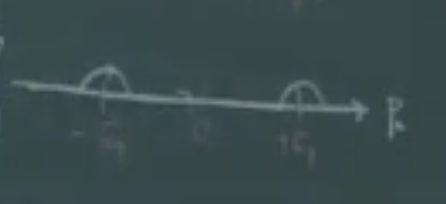
\includegraphics{img/chap3_1.png}
        \caption{(\ref{chap386})中最后一行选用的围道,当$x^{0}>y^{0}$时,为了使得大圆弧上积分为0,我们要选去圆弧经过下半平面,此时围道内有两个极点,积分结果非零,其中的负号来自于围道顺时针绕过了极点。当$x^{0}<y^{0}$时,为了大圆弧上积分结果为0,我们选取大圆弧经过上半平面,此时积分结果为0。}
        \label{fig2}
    \end{figure}
    
我们定义推迟传播子
\begin{equation}
\label{chap3retarded}
\begin{aligned}
        D_{R}(x-y)&=\theta(x^{0}-y^{0})\bra{0}\left[\phi(x),\phi(y)\right]\ket{0}\\
        &=\int_{C_{1}} \frac{d^{4}p}{(2\pi)^{4}}\frac{i}{p^{2}-m^{2}}e^{-ip(x-y)}
\end{aligned}
\end{equation}
其中$\theta(t)$为Heaviside函数,围道$C_{1}$按图(\ref{fig2})定义\footnote{这一点是值得强调的,由于我们引入的$p^{0}$的积分本身是ill-define的,事实上不同的围道选择定义了关于$p^{0}$的积分}。

下面我们简单回忆一下Green函数的基本内容。与在经典电动力学中的情况类似,我们考虑标量场,并且考虑一个有限时间区间内存在的外源$j(x)$,Lagrangian可写为
\begin{equation}
    \mathcal{L}=\frac{1}{2}(\partial_{\mu}\phi)^{2}-\frac{1}{2}m^{2}\phi^{2}+j(x)\phi(x)
\end{equation}
从而利用E-L方程我们得到含源K-G方程为
\begin{equation}
    (\partial^{2}+m^{2})\phi=j(x)
\end{equation}
在给定满足不含源K-G方程的初条件$\phi_{0}$后\footnote{因为外源只存在有限时间,我们取足够远的过去,就可以恢复之前得到的真空解(\ref{chap3phi4D}),因此不妨设$\phi_{0}$满足不含源的K-G方程},我们可以得到通解为
\begin{equation}
\label{chap3tongjie}
    \phi(x)=\phi_{0}(x)+i\int d^{4}yD_{R}(x-y)j(y)
\end{equation}
其中$D_{R}(x-y)$为经典场论中的Green函数,满足
\begin{equation}
\label{chap3st}
    (\partial^{2}+m^{2})D_{R}(x-y)=-i\delta^{4}(x-y)
\end{equation}
利用这一定义,我们可以验证通解(\ref{chap3tongjie})满足含源K-G方程:
\begin{equation}
    \begin{aligned}
    (\partial^{2}_{x}+m^{2})\phi(x)&=(\partial^{2}_{x}+m^{2})\phi_{0}(x)+i\int d^{4}y(\partial^{2}_{x}+m^{2})D_{R}(x-y)j(y)\\
    &=0+\int d^{4}y\delta^{4}(x-y)j(y)\\
    &=j(x)
    \end{aligned}
\end{equation}
其中$\partial^{2}_{x}$表示微分算符只作用于$x$变量。
直接验算可以知道,K-G场的推迟传播子(\ref{chap3retarded})也满足(\ref{chap3st})。这也可以从动量空间中看出。
从Fourier变换的定义$D_{R}(x-y)=\int \frac{d^{4}p}{(2\pi)^{4}}e^{-ip(x-y)}\tilde{D_{R}}(p)$我们可以直接从(\ref{chap3retarded})中看出,在动量空间推迟传播子的形式为
\begin{equation}
    \widetilde{D}_{R}(p)=\frac{i}{p^{2}-m^{2}}
\end{equation}
而微分算符的形式变为$-ip$,从而在动量空间,我们有
\begin{equation}
    \mathcal{F}\left[(\partial^{2}+m^{2})D_{R}(x-y)\right]=(-p^{2}+m^{2})\frac{i}{p^{2}-m^{2}}=-i=\mathcal{F}\left[-i\delta^{4}(x-y)\right]
\end{equation}

在前面的脚注中我们曾说过,围道的选择会导致不同的结果,如果我们在(\ref{chap386})中选取图(\ref{fig3_2})中的围道$C_{2}$,就可以得到向前Green函数,这一函数在$x^{0}<y^{0}$时非零,在$x^{0}>y^{0}$为0。
\begin{figure}[htbp]
    \centering
    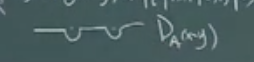
\includegraphics{img/chap3_2.png}
    \caption{第二种围道选择}
    \label{fig3_2}
\end{figure}
然而,不论是推迟Green函数还是超前Green函数,在我们这门课中用途都不是很大,我们经常用到的是下面要介绍的Feynman传播子
\begin{equation}
    D_{F}(x-y)=\int_{C_{F}} \frac{d^{4}p}{(2\pi)^{4}}\frac{i}{p^{2}-m^{2}}e^{-ip(x-y)}
\end{equation}
其选择的围道$C_{F}$如图(\ref{fig3_3})所示。由于我们在这里的积分值完全由极点的位置决定,我们可以稍微移动极点的位置使其位于$\pm(E_{\vec{p}}-i\epsilon)$,其中$\epsilon$是一个无穷小正实数\footnote{这个$\epsilon$被称为Feynman's prescription,它的引入是一个数学上的trick,在任何可观测的物理量结果中不应当出现,因此其具体的取值并不重要。},使得积分路径重新形变成$x$轴,如图(\ref{fig3_4})所示,这样我们可以将Feynman传播子写为
\begin{equation}
\begin{aligned}
     D_{F}(x-y)&=\int \frac{d^{4}p}{(2\pi)^{4}}\frac{i}{p^{2}-m^{2}+i\epsilon}e^{-ip(x-y)}\\
     \widetilde{D}_{F}(p)&=\frac{i}{p^{2}-m^{2}+i\epsilon}\\
     \end{aligned}
\end{equation}
容易验证,Feynman传播子也满足
\begin{equation}
    (\partial^{2}+m^{2})D_{F}(x-y)=-i\delta^{4}(x-y)
\end{equation}
\begin{figure}[htbp]
    \centering
    
\includegraphics{img/chap3_3.png}
    \caption{Feynman传播子选取的围道}
    \label{fig3_3}
\end{figure}

\begin{figure}[htbp]
    \centering
    
\includegraphics{img/chap3_4.png}
    \caption{形变后的Feynman传播子围道}
    \label{fig3_4}
\end{figure}

从围道选取我们可以看出,不论是$x^{0}>y^{0}$还是$x^{0}<y^{0}$,Feynman传播子都不是0,事实上,当$x^{0}>y^{0}$时
\begin{equation}
    \begin{aligned}
     D_{F}(x-y)&=-\int \frac{d^{3}p}{(2\pi)^{3}}\left.\frac{i^{2}}{2E_{\vec{p}}}e^{-ip(x-y)}\right|_{p^{0}=E_{\vec{p}}}\\
     &=D(x-y)
    \end{aligned}
\end{equation}
当$x^{0}<y^{0}$时
\begin{equation}
    \begin{aligned}
     D_{F}(x-y)&=\int \frac{d^{3}p}{(2\pi)^{3}}\left.\frac{i^{2}}{-2E_{\vec{p}}}e^{-ip(x-y)}\right|_{p^{0}=-E_{\vec{p}}}\\
     &=\int \frac{d^{3}p}{(2\pi)^{3}}\frac{1}{2E_{\vec{p}}}e^{iE_{\vec{p}}t+i\vec{p}\cdot(\vec{x}-\vec{y})}\\
      &=\int \frac{d^{3}p}{(2\pi)^{3}}\frac{1}{2E_{\vec{p}}}e^{-iE_{\vec{p}}t'+i\vec{p}\cdot(\vec{y}-\vec{x})}\\
     &=D(y-x)
    \end{aligned}
    \end{equation}
    其中在第三个等号我们做了变量替换$\vec{q}=-\vec{p}$,并仍将变量名记为$\vec{p}$,同时令$t'=-t=y^{0}-x^{0}$
从而我们有
\begin{equation}
    \begin{aligned}
     D_{F}(x-y)&=\left\{
     \begin{array}{cc}
         D(x-y),\quad x^{0}>y^{0}  \\
          D(y-x),\quad x^{0}<y^{0} \\
     \end{array}
          \right.\\
          &=\theta(x^{0}-y^{0})\bra{0}\phi(x)\phi(y)\ket{0}+\theta(y^{0}-x^{0})\bra{0}\phi(y)\phi(x)\ket{0}\\
          &\doteq\bra{0}T\left[\phi(x)\phi(y)\right]\ket{0}
    \end{aligned}
\end{equation}
最后一行我们引入了编时算符$T$,由定义,编时算符内的场算符是对易的。对于两个算符等时的情况,因为场论保护因果性,从而这两个算符之间的间隔是类空的,从而是可以对易的,其顺序不重要,从而编时算符在等时情况下的定义也是合理的。
对于多个算符我们也可以定义它们的编时乘积
\begin{equation}
    T\left[\phi(x)\phi(y)\phi(z)\right]=\left\{
 \begin{array}{c}
      \phi(x)\phi(y)\phi(z),\quad x^{0}>y^{0}>z^{0}  \\
      \phi(x)\phi(z)\phi(y),\quad x^{0}>z^{0}>y^{0}  \\
       \phi(z)\phi(x)\phi(y),\quad z^{0}>x^{0}>y^{0} \\
       \cdots \\
 \end{array}
    \right.
\end{equation}

后面的课程将会看到,Feynman传播子在利用Feynman图计算散射振幅等方面有着重要应用。事实上,Feynman图内线对应了相应粒子的Feynman传播子。因为今后我们将大量使用Feynman传播子,因此如不特殊说明,我们将Feynman传播子简称为传播子。


	\chapter{Dirac场论}
\section{Lorentz群的旋量表示}
目前所有还没被验证是错误的物理理论都满足Lorentz对称性和时空平移对称性\footnote{吐槽一下这一节比较混乱,所以我重新组织了这一节},因此仔细讨论Lorentz变换的相关性质是比较重要的,
全体Lorentz变换构成一个群,称为Lorentz群,根据场在Lorentz群作用下的行为可以对场进行分类,我们在(\ref{classfy})中已经给出了标量场、矢量场和张量场在Lorentz变换下的性质,因此一个随之而来的问题就是,在我们的分类标准下,还有没有其他的场。事实上,为了描述费米子,我们需要一种新的场,即旋量场,为此我们需要研究Lorentz群的旋量表示。
从标题看我们需要解决两个概念的问题,一个是群表示,一个是旋量,然后才可以比较好的理解Lorentz群的旋量表示。
\subsection{群表示}
所谓群表示,也就是一个群$G$到另一个群$W$的同态,在物理上我们关心的主要是群的线性表示,也就是从群$G$到一般线性群$GL(n,F)$,的同态,其中$F$是数域,在物理上通常为$\mathbb{C}$,不太确切地讲,由于群的定义是抽象的,我们可以找到用矩阵作为元素构成的一个具体的群来作为抽象群的实现。从群表示论的观点出发我们可以将群$G$中的元素看成作用在$n$维线性空间$X$上的矩阵,即线性变换,将场看作$X$中的元素,从而在Lorentz变换下场的变换性质便可以由线性变换下元素的变换性质来刻画。

作为一个例子,我们先来考虑一下熟悉的转动群$SO(3)$,其中群元素满足$R^{\top}R=RR^{\top}=I$,在转动群中元素的作用下三维向量满足
\begin{equation}
    A^{i}\longrightarrow A'^{i}(\vec{x})=R^{ij}A^{j}(R^{-1}\vec{x})
\end{equation}
其中$R^{ij}$为$3\times3$矩阵。

在上面这个例子中,我们实际上考虑了转动群$SO(3)$在三维向量空间的一个作用,由于我们在这里考虑的群本身就是一般线性群的一个子群,所以我们可以认为$SO(3)$群本身构成了一个线性表示,嵌入映射$i:SO(3)\hookrightarrow GL(\mathbb{R},3)$建立了一个同态,这样的表示称为定义表示(defining representation)。同一个群可以具有多个不同的表示,如果我们考虑下列到Lorentz群的同态
\begin{equation}
    \begin{aligned}
    \phi:SO(3) &\longrightarrow SO(1,3)\\
    R &\longrightarrow  \left(
    \begin{array}{cc}
        1 &0  \\
         0&R 
    \end{array} \right)
    \end{aligned}
\end{equation}
根据定义,这同样是转动群$SO(3)$的一个表示,事实上,将$G$中元素全部映为单位矩阵的平凡的映射也构成了一个表示,我们称之为平凡表示(trivial representation)。对于$SO(3)$的定义表示,我们可以将其中的元素参数化为
\begin{equation}
    R=e^{-i\vec{\theta}\cdot\vec{L}}
\end{equation}
其中$\vec{L}=(L_{1},L_{2},L_{3})$,$L_{i}$显示形式即为在(\ref{Lorentzgenerator})中将标号相同的矩阵删掉第一行和第一列所得到的$3\times3$矩阵。我们称$L_{i}$为转动群$SO(3)$的生成元,因为根据参数化所有的转动群中的元素可以由这三个生成元的倍数的指数映射$e^{ia_{i}L_{i}}$(不求和)生成,容易验证生成元之间满足关系
\begin{equation}
    \left[L_{i},L_{j}\right]=i\epsilon^{ijk}L_{k},\quad i,j,k=1,2,3
\end{equation}
其中$\epsilon^{ijk}$为三阶全反对称张量,选取$\epsilon^{123}=1$。
对于$SO(3)$这样,其中元素可以用一组连续参数描述的连续群称为李群\footnote{严格的定义可以参考Brain C. Hall/任意讲微分流形的书},$L_
{i}$之间的对易关系\footnote{一般而言,生成元关系满足 $\left[L_{i},L_{j}\right]=iC^{ijk}L_{k}$,我们称$C^{ijk}$为李群的结构常数,可以证明,结构常数完全确定了一个李群的结构。}定义了群的生成元之间的乘法运算,这个连同加法和数乘构成了一个代数,称为李代数\footnote{当然在李代数的定义中对于乘法运算有更多的要求,比如需要满足Jacobi恒等式等,不过我们此时暂且不需要关心这个},作为一个线性空间,李代数的一组基即为李群的生成元$L_{i}$。李代数中的元素$X$可以通过指数映射$e^{itX}$与李群中的元素对应,其中$t$是参数,一般而言指数映射既不是单射也不是满射,但是在单位元附近这是一个同胚。可以证明,对于物理上常见的情况如$SO(n)$,$U(n)$,指数映射是满射,即我们可以从生成元出发构建整个连续群;不过Lorentz群的李代数并不是满的,事实上Lorentz群分成了四个不连通的部分,其李代数通过指数映射只能映满包含单位元的那一支(恰当正时的Lorentz变换)。

另一个熟悉的例子来自自旋。我们知道对于$SU(2)$,也存在一个定义表示,Pauli矩阵构成了它的一组生成元,任意群元素具有连续的参数化形式$U=e^{-i\vec{\theta}\cdot\vec{\tau}}$,生成元之间满足
\begin{equation}
    \left[\tau_{i},\tau_{j}\right]=i\epsilon^{ijk}\tau_{k},\quad i,j,k=1,2,3
\end{equation}
其中$\vec{\tau}=\frac{\vec{\sigma}}{2}$。

经过简单的运算我们可以得到
\begin{equation}
\label{chap4U}
\begin{aligned}
    U(\vec{\theta})&=1+\sum\limits_{k=1}\limits^{\infty}\frac{1}{k!}(-i\theta_{j}\tau_{j})^{k}\\
    &={\rm cos}\frac{|\theta|}{2}I-\frac{2i\theta_{i}}{|\theta|}\tau_{i}{\rm sin}\frac{|\theta|}{2}
    \end{aligned}
\end{equation}
其中我们利用了一个常见的计算技巧
\begin{equation}
    \theta_{j}\tau_{j}\theta_{m}\tau_{m}=\frac{1}{2}\theta_{j}\theta_{m}\left\{\tau_{j},\tau_{m}\right\}=\frac{1}{2}\theta_{j}\theta_{m}\frac{1}{2}\delta^{jm}=\frac{\vec{\theta}^{2}}{4}
\end{equation}
为方便讨论,我们取$\vec{\theta}_{z}=(0,0,\theta)$,于是有
\begin{equation}
    U_{z}(\theta)={\rm cos}\frac{\theta}{2}-i\sigma_{3}{\rm sin}\frac{\theta}{2}
\end{equation}
于是我们有$U(\theta+2\pi)={\rm cos}\frac{\theta+2\pi}{2}-i\sigma_{3}{\rm sin}\frac{\theta+2\pi}{2}={\rm cos}\frac{\theta}{2}+i\sigma_{3}{\rm sin}\frac{\theta}{2}$
,因此与转动群$SO(3)$不同,$SU(2)$的作用在旋转$4\pi$后才会回到恒同映射,我们将其作用的对象(表示空间中的元素)称为旋量。
\subsection{旋量}
旋量到底是一个什么东西可能是一个令人困惑的问题,在这里我们也并不打算讨论最一般的情况,而是集中于简单的两分量旋量的情况,即一阶旋量,物理上也称为Weyl旋量,它在变换$U$下满足变换规则$\vec{s}\longrightarrow U\vec{s}$。两分量旋量$s$是具有特殊变换性质的两分量复向量,
因此完全描述它需要四个独立参数,为了讨论的方便,我们利用参数组$(r,\theta,\phi,\alpha)$将各分量表示成类似于三维空间球坐标的形式
\begin{equation}
\label{chap4define}
    \vec{s}=\left(\begin{array}{c}
         a  \\
          b
    \end{array}\right)\doteq
    \left(\begin{array}{c}
         \sqrt{r}{\rm cos}(\theta/2)e^{i(-\alpha-\phi)/2}  \\
          \sqrt{r}{\rm sin}(\theta/2)e^{i(-\alpha+\phi)/2} 
    \end{array}\right)
\end{equation}
基于这一形式我们可以给两分量旋量一个几何图像。我们可以把一个二分量旋量看作一个三维空间的刷子,刷子柄可以当作普通三维空间里的向量,用球坐标$(r,\theta,\phi)$表示,注意旋量旋转$4\pi$才会回到原点的性质,$\theta$的对应存在一个2倍关系。另一个参数$\alpha$则可以看作刷子绕刷子柄所在轴线的旋转。

今后为方便我们将一个两分量旋量写成
\begin{equation}
    \vec{s}=se^{-i\alpha/2}\left(\begin{array}{c}
         {\rm cos}(\theta/2)e^{i(-\phi)/2}  \\
          {\rm sin}(\theta/2)e^{i(\phi)/2}
    \end{array}\right)
\end{equation}
其中$s=\sqrt{r}$。

借助于(\ref{chap4define})我们可以表示出刷子柄在三维空间对应的坐标为
\begin{equation}
\label{chap4shuazi3D}
    \begin{aligned}
        r_{x}&=r{\rm sin}\theta{\rm cos}\phi=ab^{*}+ba^{*} \\ 
        r_{y}&=r{\rm sin}\theta{\rm sin}\phi=i(ab^{*}-ba^{*}) \\ 
        r_{z}&=r{\rm cos}\theta=|a|^{2}-|b|^{2} \\ 
    \end{aligned}
\end{equation}
很快我们会看到,任意一个旋量可以同一个三维向量相对应,我们称这一三维向量的方向为旋量的方向。

之前我们提到,两分量旋量具有特殊的变换性质,下面我们来考虑$SU(2)$群在旋量上的作用。下面我们将会从两个角度来证明,$SU(2)$对旋量的作用对应于旋量的旋转。

首先我们注意到,对于旋量$\vec{s}$,(\ref{chap4shuazi3D})可以借助于Pauli矩阵重新写成
\begin{equation}
\label{chap4shuazi3DPauli}
    \begin{aligned}
        r_{x}&=\vec{s}^{\dagger}\sigma_{x}\vec{s} \\ 
       r_{y}&=\vec{s}^{\dagger}\sigma_{y}\vec{s}  \\ 
        r_{z}&=\vec{s}^{\dagger}\sigma_{z}\vec{s}  \\ 
    \end{aligned}
\end{equation}
写成更紧凑的形式有
\begin{equation}
\label{chap4shuazi3Dpaulicompact}
    \vec{r}=r_{x}=\vec{s}^{\dagger}\vec{\sigma}\vec{s}=\bra{s}\vec{\sigma}\ket{s} 
\end{equation}
这一形式具有普遍性,任意一个旋量可以通过这种形式对应到一个三维矢量。

在(\ref{chap4U})中我们指出任意$SU(2)$中元素可以由Pauli矩阵的指数映射给出,因此考虑$SU(2)$群在旋量上的作用,只需要考虑下列三个特殊矩阵产生的效果。
\begin{equation}
    \begin{aligned}
        S_{x}\left(\theta\right)&=e^{i\frac{\theta}{2}\sigma_{x}}={\rm cos}\frac{\theta}{2}I+i\sigma_{x}{\rm sin}\frac{\theta}{2}=\left(\begin{array}{cc}
           {\rm cos}\frac{\theta}{2}  & i{\rm sin}\frac{\theta}{2} \\
            i{\rm sin}\frac{\theta}{2} & {\rm cos}\frac{\theta}{2}
        \end{array}\right)\\
         S_{y}\left(\theta\right)&=e^{i\frac{\theta}{2}\sigma_{y}}={\rm cos}\frac{\theta}{2}I+i\sigma_{y}{\rm sin}\frac{\theta}{2}=\left(\begin{array}{cc}
           {\rm cos}\frac{\theta}{2}  & {\rm sin}\frac{\theta}{2} \\
            -{\rm sin}\frac{\theta}{2} & {\rm cos}\frac{\theta}{2}
        \end{array}\right)\\
         S_{z}\left(\theta\right)&=e^{i\frac{\theta}{2}\sigma_{z}}={\rm cos}\frac{\theta}{2}I+i\sigma_{z}{\rm sin}\frac{\theta}{2}=\left(\begin{array}{cc}
           e^{i\frac{\theta}{2}}  & 0 \\
           0 & e^{-i\frac{\theta}{2}} 
        \end{array}\right)\\
    \end{aligned}
\end{equation}

作为一个例子,我们考虑$\vec{s}'=S_{x}\vec{s}$,
从而根据(\ref{chap4shuazi3Dpaulicompact}),其对应的三维向量为
\begin{equation}
    \vec{r}'=\bra{s'}\vec{\sigma}\ket{s'}=\bra{s}e^{-i\frac{\theta}{2}\sigma_{x}}\vec{\sigma}e^{i\frac{\theta}{2}\sigma_{x}}\ket{s}
\end{equation}
写成分量形式有
\begin{equation}
    \begin{aligned}
        x'&=\bra{s}e^{-i\frac{\theta}{2}\sigma_{x}}\sigma_{x}e^{i\frac{\theta}{2}\sigma_{x}}\ket{s}\\
        &=\bra{s}\sigma_{x}e^{-i\frac{\theta}{2}\sigma_{x}}e^{i\frac{\theta}{2}\sigma_{x}}\ket{s}\\
        &=\bra{s}\sigma_{x}\ket{s}\\
        &=x\\
        y'&=\bra{s}e^{-i\frac{\theta}{2}\sigma_{x}}\sigma_{y}e^{i\frac{\theta}{2}\sigma_{x}}\ket{s}\\
        &=\bra{s}\left(\text{cos}\frac{\theta}{2}I+i\sigma_{x}\text{sin}\frac{\theta}{2}\right)\sigma_{y}\left({\rm cos}\frac{\theta}{2}I+i\sigma_{x}{\rm sin}\frac{\theta}{2}\right)\ket{s}\\
        &=\bra{s}\sigma_{y}(\text{cos}\theta+i\sigma_{x}\text{sin}\theta)\ket{s}\\
        &=\text{cos}\theta\bra{s}\sigma_{y}\ket{s}+i\text{sin}\theta\bra{s}\sigma_{y}\sigma_{x}\ket{s}\\
        &=y\text{cos}\theta+z\text{sin}\theta \\
        z'&=\bra{s}e^{-i\frac{\theta}{2}\sigma_{x}}\sigma_{z}e^{i\frac{\theta}{2}\sigma_{x}}\ket{s}\\
        &=\text{cos}\theta\bra{s}\sigma_{z}\ket{s}+i\text{sin}\theta\bra{s}\sigma_{z}\sigma_{x}\ket{s}\\
         &=z\text{cos}\theta-y\text{sin}\theta \\
    \end{aligned}
\end{equation}
从而我们得到
\begin{equation}
    \vec{r}'=R_{x}\left(\theta\right)\vec{r}
\end{equation}
其中
\begin{equation}
    R_{x}\left(\theta\right)=\left(
    \begin{array}{ccc}
         1&0&0  \\
         0&\text{cos}\theta& \text{sin}\theta\\
          0&\text{-sin}\theta& \text{cos}\theta\\
    \end{array}
    \right)
\end{equation}
是$SO(3)$中的元素。类似地我们可以得到$S_{y}\left(\theta\right),S_{z}\left(\theta\right)$分别对应$R_{y}\left(\theta\right),R_{z}\left(\theta\right)$,注意其中角度的二倍关系。我们在上一节中已经指出,$L_{i}$和$\sigma_{i}$分别是$SO(3)$和$SU(2)$的生成元,因此
\begin{equation}
\begin{aligned}
    \Phi:SU(2)&\longrightarrow SO(3)\\
    S=e^{i\vec{\sigma}\cdot\frac{\vec{\theta}}{2}}&\longrightarrow R=e^{i\vec{L}\cdot\vec{\theta}}
    \end{aligned}
\end{equation}
构成了两群之间任意元素的对应关系。

由于$SU(2)$群是$2\times2$矩阵,从而如果$U\in SU(2)$,那么$-U\in SU(2)$,从上面的推导过程我们可以发现$\{U,-U\}$都对应于同一个$SO(3)$中的元素,于是我们称$SU(2)$是$SO(3)$的一个二叠覆盖(double cover)。从李代数的角度来看,$SO(3)$同$SU(2)$结构的相似性可以从它们的生成元满足相似的对易关系看出。

至此我们发现,$SU(2)$群对旋量的作用相当于$SO(3)$群对旋量所对应的矢量的作用,即$SU(2)$群转动了旋量$\vec{s}$的方向。上述对应也可以采用从矢量出发的另一种路径,这一种方法更容易推广,我们也把它列在下面。

Step1.我们将一个三维向量$\vec{r}=(x,y,z)$对应到无迹厄米矩阵
\begin{equation}
\label{chap4step1}
    X=\vec{r}\cdot\vec{\sigma}=x\sigma_{x}+y\sigma_{y}+z\sigma_{z}=\left(\begin{array}{cc}
        z & x-iy \\
        x+iy & -z
    \end{array}\right)
\end{equation}
其行列式$\text{det}(X)=-(x^{2}+y^{2}+z^{2})=-|\vec{r}|^{2}$。
我们定义$SU(2)$在无迹厄米矩阵上的作用为
\begin{equation}
    X'=T_{U}(X)=UXU^{\dagger}
\end{equation}
显然$X'$仍然是厄米无迹矩阵,由于Pauli矩阵构成$SU(2)$群的一组基,从而有
\begin{equation}
    X'=\vec{r}\cdot\vec{\sigma}=x'\sigma_{x}+y'\sigma_{y}+z'\sigma_{z}
\end{equation}
由于$\text{det}X'=\text{det}(UXU^{\dagger})=\text{det}(U^{\dagger}UX)=\text{det}X$,从而$\vec{r}\longrightarrow \vec{r}'$保持模不变,从而$T_{U}$对$\vec{r}$的变换效果只能是旋转或反射变换的复合,我们考察$U_{z}=e^{i\frac{\theta}{2}\sigma_{z}}$,通过计算可知
\begin{equation}
    T_{U_{z}}=e^{i\frac{\theta}{2}\sigma_{z}}Xe^{-i\frac{\theta}{2}\sigma_{z}}=\left(
    \begin{array}{cc}
        z & e^{i\theta}(x-iy) \\
        e^{-i\theta}(x+iy) & z
    \end{array}\right)
\end{equation}
从而我们有
\begin{equation}
    \begin{aligned}
    x'&=x\text{cos}\theta+y\text{sin}\theta\\
     y'&=-x\text{sin}\theta+y\text{cos}\theta\\
     z'&=z
    \end{aligned}
\end{equation}
类似地我们可以验证其他分量的情况,从而我们可以得知$T_{U}$对$X$所对应的三维向量的效果是转动。

Step2.我们将一个无迹厄米矩阵对应到两分量旋量。事实上,我们下面将要证明,任何一个旋量$\vec{s}$都是一个无迹厄米矩阵$S$的特征值为1的特征向量。我们采用构造性的证明。由于我们要求$S$是厄米的,从而由高代中熟知的结论我们知道$S$的特征值为实数且不同特征值的特征向量正交,此外,我们知道厄米矩阵所有的特征向量组成了一组基。倘若
\begin{equation}
    \vec{s}=\left(\begin{array}{c}
         a  \\
         b 
    \end{array}\right)
\end{equation}
是$S$特征值为1的特征向量,则我们应该有与之正交的矢量
\begin{equation}
    \vec{s'}=\left(\begin{array}{c}
         -b^{*}  \\
         a^{*} 
    \end{array}\right)
\end{equation}
为$S$的另一特征向量,且特征值为$-1$,事实上,如果$\vec{s}'$的特征值也为1,我们记矩阵
\begin{equation}
    V=\frac{1}{|\vec{s}|}\left(\begin{array}{cc}
        \vec{s} &  \vec{s}'\\
    \end{array}\right)
    =\frac{1}{|\vec{s}|}
    \left(\begin{array}{cc}
        a &  -b^{*}\\
        b & a^{*}
    \end{array}\right)
\end{equation}
则有
\begin{equation}
    SV=VI
\end{equation}
由于$S$的所有特征向量构成一组基,则$V$可逆,从而$S=I$,矛盾。

于是$S$有两个特征向量分别对应特征值为$\pm 1$,可以写成
\begin{equation}
    SV=V\sigma_{z}
\end{equation}
从中解得\footnote{容易证明,最终结果$S$与在构造$V$时$\vec{s}$和$\vec{s}'$的排列次序无关}
\begin{equation}
    S=V\sigma_{z}V^{\dagger}=\frac{1}{s^{2}}\left(
    \begin{array}{cc}
       |a|^{2}-|b|^{2}  & 2ab^{*} \\
        2ba^{*} & |b|^{2}-|a|^{2}
    \end{array}\right)=\frac{1}{|r|}\left(
    \begin{array}{cc}
       r_{z}  & r_{x}-ir_{y} \\
        r_{x}+ir_{y} & -r_{z}
    \end{array}\right)=\vec{n}\cdot\vec{\sigma}
\end{equation}
其中利用了(\ref{chap4shuazi3D}),并采用记号$\vec{n}=\frac{1}{|r|}\left(r_{x},r_{y},r_{z}\right)=\frac{\bra{s}\vec{\sigma}\ket{s}}{s^{2}}$。$S$以$\vec{s}$为特征向量,且特征值为1,由证明过程可以看出$S$的选择是唯一的。同(\ref{chap4step1})相比较,可以得知$S$所对应的三维向量的方向$\vec{n}$即为旋量$\vec{s}$的方向,即三维矢量可以对应到一个相同方向的旋量。

换句话说,我们证明了,对于任意单位向量$\vec{n}$,存在唯一无迹厄米矩阵$X=\vec{n}\cdot\vec{\sigma}$,满足$X$有一个特征值为1的特征向量,这是一个旋量,其方向与$\vec{n}$相同。

现在我们再来讨论旋量的变换的问题。对于$U\in SU(2)$,我们有$\vec{s}'=U\vec{s}$,注意到
\begin{equation}
    (USU^{\dagger})\vec{s}'=(USU^{\dagger})U\vec{s}=US\vec{s}=U\vec{s}=\vec{s}'
\end{equation}
其中$S$为$\vec{s}$所对应的厄米矩阵。于是我们有
\begin{equation}
    S'=USU^{\dagger}
\end{equation}
根据我们在Step1中的讨论,这对应着$S$对应的三维向量$\vec{r}$的转动,从而对应着旋量$\vec{s}$的方向的转动。

上面我们用两种方式讨论了旋量的空间变换,下面我们将上述讨论推广到boost。
我们考虑厄米矩阵(此时不再要求无迹)
\begin{equation}
    X=tI+x\sigma_{x}+y\sigma_{y}+z\sigma_{z}=\left(\begin{array}{cc}
        t+z &x-iy  \\
        x+iy & t-z
    \end{array}\right)
\end{equation}
其行列式满足$\text{det}X=t^{2}-x^{2}-y^{2}-z^{2}$,这恰好是四矢量$(t,\vec{r})$的长度。由于我们不要求迹具有不变性,从而我们考虑行列式为1的复矩阵$U\in SL(2,\mathbb{C})$,并考虑变换
\begin{equation}
    T_{U}(X)=UXU^{\dagger}
\end{equation}
显然变换前后$\text{det}X$是不变量。
容易验证$SL(2,\mathbb{C})$的一组生成元为$\sigma_{i},-i\sigma_{i}$,其中空间部分我们已经在前面处理过,对于boost部分(记作$B_{i}$),我们考虑一个例子
\begin{equation}
    B_{z}=e^{-i\frac{\beta}{2}(-i\sigma_{z})}=e^{-\frac{\beta}{2}\sigma_{z}}=\left(\begin{array}{cc}
       e^{-\frac{\beta}{2}}  & 0 \\
         0& e^{\frac{\beta}{2}} 
    \end{array}\right)=\text{cosh}(\beta)I-\sigma_{z}\text{sinh}\beta
\end{equation}
考虑$T_{B_{z}}$,计算可得,在这一变化下,$X'$对应的四矢量$r'$满足$\vec{r}'=K_{z}r$,其中
\begin{equation}
    K_{z}=\left(\begin{array}{cccc}
         \text{cosh}\beta&0&0&-\text{sinh}\beta  \\
         0&1&0&0\\
         0&0&1&0\\
         -\text{sinh}\beta&0&0&\text{cosh}\beta
    \end{array}\right)
\end{equation}
类似可以验证其他两个方向的boost。与空间部分相类似,$SL(2,\mathbb{C})$构成了Lorentz群的一个二叠映射。
于是我们可以将旋量的空间转动和boost统一写成
\begin{equation}
\label{chap4SL2}
    U=e^{i\frac{\vec{\theta}\cdot\vec{\sigma}}{2}-\frac{\vec{\beta}\cdot\vec{\sigma}}{2}}
\end{equation}
$U$是$SL(2,\mathbb{C})$中的元素。顺便一提,按$X\longrightarrow UXU^{\dagger}$变换的旋量称为2阶旋量,我们上面的讨论表明,二阶旋量与矢量有相同的变换规则。
\subsection{Lorentz群的旋量表示}
首先来讨论Lorentz群的李代数。我们需要知道Lorentz群生成元(\ref{Lorentzgenerator})的对易关系。考虑到Lorentz群的各种表示要满足相同的对易关系,因此我们可以通过Lorentz群的任意一个表示来得到普遍的对易关系。下面来考虑作用到函数空间上的无穷维表示。对于转动群,角动量算符为$\vec{J}=\vec{x}\times\vec{p}=\vec{x}\times(-i\nabla)$,我们可以定义
\begin{equation}
    J^{ij}=-i(x^{i}\nabla^{j}-x^{j}\nabla^{i})
\end{equation}
这样我们可以恢复角动量算符的定义$J^{3}=J^{12}(cyc.)$。从这一形式出发,我们可以很自然地推广到四维的情况
\begin{equation}
    J^{\mu\nu}=i(x^{\mu}\partial^{\nu}-x^{\nu}\partial^{\mu})
\end{equation}
这样我们得到了6个独立的生成元,当$\mu,\nu=1,2,3$时,我们恢复了三维转动的生成元,当$\mu,\nu$有一个等于0时,我们得到了boost的生成元。直接计算可以得到表示空间为无穷维的Lorentz群表示的生成元的对易关系为
\begin{equation}
\label{chap4commurela}
    \left[J^{\mu\nu},J^{\rho\sigma}\right]=i(g^{\nu\rho}J^{\mu\sigma}-g^{\mu\rho}J^{\nu\sigma}-g^{\nu\sigma}J^{\mu\rho}+g^{\mu\sigma}J^{\nu\rho})
\end{equation}

利用这一生成元,我们可以用6个实参数来描述Lorentz变换
\begin{equation}
    \Lambda^{\alpha}_{\;\;\beta}=\left[e^{-\frac{i}{2}\omega_{\mu\nu}J^{\mu\nu}}\right]^{\alpha}_{\;\;\beta}
\end{equation}
其中$\Lambda^{\alpha}_{\;\;\beta}$及$J^{\mu\nu}$满足的对易关系的形式 不仅仅局限于无穷维Lorentz群表示的情况,也可以适用于有限维表示。
对于Lorentz群的一个有限维表示$M(\Lambda)$,场$\Phi$按Lorentz群变换的性质可以表示为
\begin{equation}
    \Phi \xrightarrow{\Lambda} \Phi'=M(\Lambda)\Phi
\end{equation}
对于矢量表示,当$\Lambda$的参数变化$2\pi$时,得到相同的变换,对于旋量表示,则需要变化$4\pi$才可以回到原来的表示。根据我们上一节中的讨论,1阶旋量按$SL(2,\mathbb{C})$中的元素进行变换。

首先,作为一个例子,我们来考虑一组$4\times4$矩阵\footnote{$g^{\mu}_{\;\;\nu}=g^{\mu\alpha}g_{\alpha\nu}=\delta^{\mu}_{\;\;\nu}$}
\begin{equation}
\label{chap4vectorgene}
    \left[J^{\mu\nu}\right]_{\alpha\beta}=i\left(\delta^{\mu}_{\;\;\alpha}\delta^{\nu}_{\;\;\beta}-\delta^{\mu}_{\;\;\beta}\delta^{\nu}_{\;\;\alpha}\right)
\end{equation}
容易验证,这组矩阵满足对易关系(\ref{chap4commurela}),而且$J^{\mu\nu}$是反对称的\footnote{这并不是一个巧合。事实上,考虑无穷小变换($\omega_{\mu\nu}$是参数),有$\Lambda^{\alpha}_{\;\;\beta}=\delta^{\alpha}_{\;\;\beta}-\frac{i}{2}\omega_{\mu\nu}\left[J^{\mu\nu}\right]^{\alpha}_{\;\;\beta}+o(\omega^{2})$,代入Lorentz变换的要求$ g_{\mu\nu}\Lambda^{\mu}_{\;\;\rho}\Lambda^{\nu}_{\;\;\sigma}=g_{\rho\sigma}$,并考虑到$\omega_{\mu\nu}$的任意性可以得到结论。随后利用$J^{\mu\nu}$的反对称性,可以发现$\omega_{\mu\nu}$中的对称部分不会对求和$\omega_{\mu\nu}J^{\mu\nu}$产生影响,从而不妨设$\omega_{\mu\nu}$也是反对称的张量。}。。这是Lorentz群矢量表示的生成元,事实上,我们考虑无穷小变换对于四矢量的作用
\begin{equation}
\label{chap4examp}
    V^{\alpha}\longrightarrow \left(\delta^{\alpha}_{\;\;\beta}-\frac{i}{2}\omega_{\mu\nu}\left[J^{\mu\nu}\right]^{\alpha}_{\;\;\beta}\right)V^{\beta}
\end{equation}
可以验证这是四矢量在Lorentz变换下的行为的无穷小形式,例如,取$\omega_{12}=-\omega_{21}=\theta$,其余参数为0,则(\ref{chap4examp})的矩阵形式为
\begin{equation}
    V\longrightarrow \left(\begin{array}{cccc}
        1&0 &0 &0 \\
          0&1 &-\theta &0\\
           0&\theta &1 &0\\
            0&0 &0 &1
    \end{array}\right)V
\end{equation}
这是绕$z$轴作空间旋转的矩阵的无穷小形式,取$\omega_{01}=-\omega_{10}=\beta$,其余参数为0,则(\ref{chap4examp})的矩阵形式为
\begin{equation}
    V\longrightarrow \left(\begin{array}{cccc}
        1&\beta &0 &0 \\
          \beta&1 &0 &0\\
           0&0 &1 &0\\
            0&0 &0 &1
    \end{array}\right)V
\end{equation}
这是沿$x$轴方向的boost的无穷小形式,类似地我们可以得到其他参数组合的结果,这样就证明了我们给出的矩阵构成了Lorentz群矢量表示的生成元。

如果我们要构造Lorentz群的一个旋量表示,我们需要显式地构造出满足(\ref{chap4commurela})的生成元$J^{\mu\nu}$,在构造过程中我们要求$J^{\mu\nu}=-J^{\nu\mu}$
假设存在四个$n\times n$方阵$\gamma^{\mu}$,$\mu=0,1,2,3$,满足
\begin{equation}
\label{chap4condition}
    \left\{\gamma^{\mu},\gamma^{\nu}\right\}=2g^{\mu\nu}I
\end{equation}
利用满足这一关系的gamma矩阵我们可以构造
\begin{equation}
    S^{\mu\nu}=\frac{i}{4}\left[\gamma^{\mu},\gamma^{\nu}\right]
\end{equation}
通过构造我们立马可以得出$S^{\mu\nu}$是反对称的。
经过简单的计算,我们有
\begin{equation}
    \left[S^{\mu\nu},S^{\rho\sigma}\right]=i(g^{\nu\rho}S^{\mu\sigma}-g^{\mu\rho}S^{\nu\sigma}-g^{\nu\sigma}S^{\mu\rho}+g^{\mu\sigma}S^{\nu\rho})
\end{equation}
这与(\ref{chap4commurela})形式相同\footnote{我们称$\gamma^{\mu}$构成的代数为Dirac代数,这是一个16维的代数(一组可能的基底包括$I$,$\gamma^{\mu}$,以及gamma矩阵的线性无关乘积$\gamma^{\mu}\gamma^{\nu},\;\gamma^{\mu}\gamma^{\nu}\gamma^{\rho},\;\gamma^{\mu}\gamma^{\nu}\gamma^{\rho}\gamma^{\sigma}$)。},于是$S^{\mu\nu}$构成了Lorentz群李代数的一组生成元。下面的问题便是寻找满足(\ref{chap4condition})的一组$n\times n$矩阵。与在第一章的论证类似,我们可以说明不存在$2\times 2$矩阵满足条件。但是如果我们取$\gamma^{i}=i\sigma^{i}$,可以验证有
$\left\{\gamma^{i},\gamma^{j}\right\}=-2\delta^{ij}$,等式右边恰好是度规张量的空间部分,这启示我们应该从Pauli矩阵出发试图构建满足条件的gamma矩阵。一个聪明的想法是考虑$n=4$的情况,令
\begin{equation}
\label{chap4weyl}
    \begin{aligned}
    \gamma^{0}=\left(\begin{array}{cc}
       0  & I_{2} \\
       I_{2}  & 0
    \end{array}\right),\quad
    \gamma^{i}=\left(\begin{array}{cc}
       0  & \sigma^{i} \\
       -\sigma^{i}  & 0
    \end{array}\right)
    \end{aligned}
\end{equation}
容易验证这满足反对易条件(\ref{chap4condition}),我们称(\ref{chap4weyl})中写出的Lorentz群表示为手征Weyl表示。事实上,在四维情况下,上述选取并不是唯一的,对于任意可逆矩阵,我们有定义$\tilde{\gamma}^{\mu}=U\gamma^{\mu} U^{-1}$,
则有
\begin{equation}
    \left\{\tilde{\gamma}^{\mu},\tilde{\gamma}^{\nu}\right\}=U\left\{\gamma^{\mu},\gamma^{\nu}\right\} U^{-1}=g^{\mu\nu}UIU^{-1}=g^{\mu\nu}
\end{equation}
我们选用的手征Weyl表示在处理高能粒子($|\vec{v}|\sim 1$,$\;E\gg m_{0}$)时会带来方便,也是这门课中我们所选用的表示。除此之外,还有其他两种常用表示。

Dirac-Pauli表示:
\begin{equation}
\label{chap4dirac}
    \begin{aligned}
    \gamma^{0}=\left(\begin{array}{cc}
        I_{2}&0 \\
       0&-I_{2} 
    \end{array}\right),\quad
    \gamma^{i}=\left(\begin{array}{cc}
       0  & \sigma^{i} \\
       -\sigma^{i}  & 0
    \end{array}\right)
    \end{aligned}
\end{equation}
这一表示在处理非相对论性($|\vec{v}|\ll,\;E\sim m_{0}$ )粒子时比较方便\footnote{这也是Dirac在提出Dirac方程时使用的表示}。

Majorana表示:
\begin{equation}
\label{chap4Majorana}
    \begin{aligned}
    \gamma^{0}&=\left(\begin{array}{cc}
        0&\sigma_{2} \\
       \sigma_{2}&0 
    \end{array}\right),\quad
    \gamma^{1}=\left(\begin{array}{cc}
        i\sigma^{3}&0 \\
         0&i\sigma^{3} 
    \end{array}\right)\\
    \gamma^{2}&=\left(\begin{array}{cc}
        0&-\sigma_{2} \\
       \sigma_{2}&0 
    \end{array}\right),\quad
    \gamma^{3}=\left(\begin{array}{cc}
        -i\sigma^{1}&0 \\
         0&-i\sigma^{1} 
    \end{array}\right)\\
    \end{aligned}
\end{equation}
这一表示中每个矩阵都是纯虚数矩阵,在处理Majorana费米子时比较方便。这是一种电中性费米子,其反粒子是自身。目前人们猜测中微子可能是一种Majorana费米子(当然也可能是一种Dirac费米子)。

事实上,对于绝大多数物理量而言,gamma的具体形式并不会影响最后的结果,尤其是对于可观测的物理量而言,我们出于计算的方便而选取的具体的形式不应该对可观测量的计算结果有影响。

直接从Dirac代数的对易关系出发,我们有
\begin{equation}
\label{chap4dirac11}
    \begin{aligned}
       (\gamma^{0})^{2}&=I\\
          (\gamma^{i})^{2}&=-I
       \end{aligned}
\end{equation}
从Weyl表示出发,我们有以下结论\footnote{这一结论并不能从Dirac代数的对易关系直接得到,事实上,之前我们已经证明,在相似变换下不改变对易关系,而幺正性在相似变换下并不会被保持。当然(\ref{chap4hermi})不依赖于具体的表示,不过这一点的证明比较复杂,需要用到gamma矩阵的幺正性,而这依赖于群表示论中的结论:有限群的任意有限维表示$D(g)$等价于一个幺正的有限维表示$D'(g)$,即存在一个不依赖于群元$g$的可逆矩阵$S$,使得$D'(g)=SD(g)S^{-1}$为幺正矩阵。注意到所有的gamma矩阵在矩阵乘法下生成了一个有限群,从而我们总是可以人为选取一组幺正的gamma矩阵,从而有$(\gamma^{\mu})^{\dagger}=(\gamma^{\mu})^{-1}$,之后利用(\ref{chap4dirac11})可得结论。}
\begin{equation}
\label{chap4hermi}
    \begin{aligned}
    \left.\begin{array}{cc}
         (\gamma^{0})^{\dagger}=\gamma^{0}\\
          (\gamma^{i})^{\dagger}=-\gamma^{i}\\
    \end{array}\right\}&(\gamma^{\mu})^{\dagger}=\gamma^{0}\gamma^{\mu}\gamma^{0}\\
       \end{aligned}
\end{equation}
为方便,我们写出Weyl表象下旋量表示生成元的形式。
\begin{equation}
    \begin{aligned}
    S^{ij}=\frac{i}{4}\left[\gamma^{i},\gamma^{j}\right]=\frac{1}{2}\epsilon^{ijk}\left(\begin{array}{cc}
      \sigma^{k}   &0  \\
       0  & \sigma^{k}
    \end{array}\right)\doteq \frac{1}{2}\epsilon^{ijk}\Sigma^{k}\\
    S^{0i}=\frac{i}{4}\left[\gamma^{0},\gamma^{i}\right]=-\frac{i}{2}\left(\begin{array}{cc}
      \sigma^{i}   &0  \\
       0  & -\sigma^{i}
    \end{array}\right)
    \end{aligned}
\end{equation}
我们看到空间部分和boost生成元都是分块对角矩阵,这暗示我们将要引入的Dirac场的前两个分量会发生混合,后两个分量也会发生混合,但是它们之间是相互独立的。换句话说,Dirac场$\psi$是两个1阶旋量直积生成的\footnote{用表示论的语言来描述,Dirac旋量表示是Lorentz群的一个可约表示,直观来说,这意味着每一个群元素对应的矩阵$D(g)$都可以以相同的形式同时分块对角,从而一个有限维可约表示可以由多个不可约表示直和形成。可以证明Weyl旋量表示是不可约的。},记为
\begin{equation}
   \psi=\left(\begin{array}{cc}
        \chi_{L}  \\
         \phi_{R}
   \end{array}\right) 
\end{equation}
我们称$\phi_{R}$为右手分量,称$\chi_{R}$为左手分量,其名称的意义将在后面看到。
同样在后面会看到,这构成了Lorentz群的一个可约表示。

利用生成元,我们可以写出旋量表示对应的矩阵
\begin{equation}
\label{chap4spinor}
    \Lambda_{\frac{1}{2}}=e^{-\frac{i}{2}\omega_{\mu\nu}S^{\mu\nu}}
\end{equation}

可以证明,旋量表示满足下列对易关系\footnote{证明过程中你可能会用到$\left[A,\left[B,C\right]\right]=\left\{A,B\right\}C+C\left\{A,B\right\}-B\left\{A,C\right\}-\left\{A,C\right\}B$}。
\begin{equation}
\begin{aligned}
   \left[\gamma^{\sigma},S^{\mu\nu}\right] &=i(g^{\sigma\mu}\gamma^{\nu}-g^{\sigma\nu}\gamma^{\mu})\\
   &=i(g^{\sigma\mu}g^{\nu}_{\;\;\alpha}-g^{\sigma\nu}g^{\mu}_{\;\;\alpha})\gamma^{\alpha}\\
   &=\left[J^{\mu\nu}\right]^{\sigma}_{\;\;\alpha}\gamma^{\alpha}
   \end{aligned}
\end{equation}
其中$\left[J^{\mu]nu}\right]$是(\ref{chap4vectorgene})中的矢量表示生成元。
利用这一对易关系我们可以得到下列重要的结论
\begin{equation}
\label{chap4spinorimpor}
    \Lambda_{\frac{1}{2}}^{-1}\gamma^{\sigma}\Lambda_{\frac{1}{2}}=\Lambda^{\sigma}_{\;\;\rho}\gamma^{\rho}
\end{equation}
事实上,考虑无穷小变换
\begin{equation}
\label{chap4lambda12}
    \Lambda_{\frac{1}{2}}=1-\frac{i}{2}\omega_{\mu\nu}S^{\mu\nu}+o(\omega^{2})
\end{equation}
代入(\ref{chap4lambda12})左边我们有
\begin{equation}
    \begin{aligned}
    &(1+\frac{i}{2}\omega_{\mu\nu}S^{\mu\nu})\gamma^{\sigma}(1-\frac{i}{2}\omega_{\mu\nu}S^{\mu\nu})\\
    =&\gamma^{\sigma}-\frac{i}{2}\omega_{\mu\nu}\left[\gamma^{\sigma},S^{\mu\nu}\right]\\
    =&\gamma^{\sigma}-\frac{i}{2}\omega_{\mu\nu}\left[J^{\mu\nu}\right]^{\sigma}_{\;\;\alpha}\gamma^{\alpha}\\
    =&(g^{\sigma}_{\;\;\rho}-\frac{i}{2}\omega_{\mu\nu}\left[J^{\mu\nu}\right]^{\sigma}_{\;\;\alpha}g^{\alpha}_{\;\;\rho})\gamma^{\rho}\\
    =&\left(1-\frac{i}{2}\omega_{\mu\nu}J^{\mu\nu}\right)^{\sigma}_{\;\;\rho}\gamma^{\rho}\\
    =&\Lambda^{\sigma}_{\;\;\rho}\gamma^{\rho}
    \end{aligned}
\end{equation}
这就在单位元邻域内证明了结论。
归纳可知
\begin{equation}
    \left(\Lambda_{\frac{1}{2}}^{-1}\right)^{n}\gamma^{\sigma}\left(\Lambda_{\frac{1}{2}}\right)^{n}=\left(\Lambda^{n}\right)^{\sigma}_{\;\;\rho}\gamma^{\rho}
\end{equation}
从而对于有限的$\omega_{\mu\nu}$,结论依然成立。在下一节中我们将利用这一结论证明Dirac方程的Lorentz不变性。
\section{Dirac方程的构造}
在第一章中,我们从相对论性量子力学出发得到了Dirac方程,那里的波函数$\psi$具有几率诠释。现在我们从经典场论的出发,根据对称性来重新构造Dirac方程,这样得到的方程具有完全不同的物理诠释。
考虑场$\psi$按旋量表示(\ref{chap4spinor})变换,即有
\begin{equation}
\psi(x) \xrightarrow{x'=\Lambda x} \psi'(x)=\Lambda_{\frac{1}{2}}\psi(\Lambda^{-1}x)
\end{equation}
上面我们在同一个坐标点写出了变换后场的形式。我们称满足这样变换关系的场为旋量场,也称为Dirac场。注意$\Lambda$和$\Lambda_{\frac{1}{2}}$均为$4\times 4$矩阵,但是含义不同,前者作用的空间是四维时空,后者作用的空间是$\psi=(\psi_{1},\psi_{2},\psi_{3},\psi_{4})^{\top}$四个分量构成的内禀空间。

与矢量情况下类似,我们考虑旋量表示的某一个分量的变换,来获得旋量在Lorentz变换下的直接的印象。在(\ref{chap4spinor})中取$\omega_{12}=-\omega_{21}=\theta_{z}$,其他分量为0,我们有
\begin{equation}
\label{chap4exam3}
    \Lambda_{\frac{1}{2}}=e^{-\frac{i}{2}\omega_{12}S^{12}-\frac{i}{2}\omega_{21}S^{21}}=e^{-i\theta_{z} S^{12}}=\left(\begin{array}{cc}
       e^{-\frac{i}{2}\theta_{z}\sigma_{3}}  &0  \\
        0 & e^{-\frac{i}{2}\theta_{z}\sigma_{3}} 
    \end{array}\right)
\end{equation}
其中$e^{-\frac{i}{2}\theta_{z}\sigma_{3}}$是我们在(\ref{chap4SL2})中给出的一阶旋量的变换矩阵,由此可见,此时$\Lambda_{\frac{1}{2}}$分别对Dirac场右手分量和左手分量做变换。从(\ref{chap4exam3})我们可以看出,$\Lambda_{\frac{1}{2}}(2\pi)=-I=\Lambda_{\frac{1}{2}}(0)$,这再一次表明了旋量不同于四矢量的变换规则。

下面来构造Dirc场的Lagrangian。

因为我们要求$\mathcal{L}$为Lorentz标量,所以我们需要了解构建Lagrangian的各元素的变换规则。从我们在标量场的经验我们猜测$\psi^{\dagger}\psi$是可能的Lorentz标量的候选,不过事实并非如此,$\psi^{\dagger}\psi \rightarrow \psi^{\dagger}\Lambda_{\frac{1}{2}}^{\dagger}\Lambda_{\frac{1}{2}}\psi $,而$\Lambda_{\frac{1}{2}}$并非是幺正矩阵\footnote{由于Lorentz群不是紧致的,从而其不存在忠实的有限维幺正表示。事实上,三维转动群是紧群,从而生成元$S^{ij}$是厄米的,其对应的$\Lambda_{\frac{1}{2}}$是幺正矩阵;而boost生成元$S^{0i}$是反厄米的,其对应的$\Lambda_{\frac{1}{2}}$不是幺正矩阵。通常而言,在量子力学中我们要求对称性所对应的算符是幺正的,以保持几率守恒,注意这里$\Lambda_{\frac{1}{2}}$的非幺正性不会产生物理上的困难,因为其作用的对象是经典Dirac场而不是物理态,从而不存在几率诠释。后面我们会看到,Lorentz群存在幺正的无穷维表示,从而其作用在量子态所在的无穷维Hilbert空间上时,不存在幺正性的困难。},从而$\psi^{\dagger}\psi$不是Lorentz不变量。如果我们定义
\begin{equation}
    \overline{\psi}=\psi^{\dagger}\gamma^{0}
\end{equation}
下面将会证明$\overline{\psi}\psi$是Lorentz标量。

利用(\ref{chap4hermi})我们有$\gamma^{0}(S^{\mu\nu})^{\dagger}\gamma^{0}=S^{\mu\nu}$,随即我们有
\begin{equation}
    \gamma^{0}(\Lambda_{\frac{1}{2}})^{\dagger}\gamma^{0}=\Lambda_{\frac{1}{2}}^{-1}
\end{equation}
于是
\begin{equation}
    \begin{aligned}
        \overline{\psi}\psi&\rightarrow \psi'^{\dagger}\gamma^{0}\psi'\\
        &=\psi^{\dagger}\Lambda_{\frac{1}{2}}^{\dagger}\gamma^{0}\Lambda_{\frac{1}{2}}\psi\\
        &=\psi^{\dagger}\gamma^{0}\Lambda_{\frac{1}{2}}^{-1}\Lambda_{\frac{1}{2}}\psi\\
        &=\overline{\psi}\psi
    \end{aligned}
\end{equation}

下面我们试图构造Lorentz不变的导数项。
注意到
\begin{equation}
    \overline{\psi}\gamma^{\mu}\psi\xlongrightarrow{\Lambda}\overline{\psi}\Lambda_{\frac{1}{2}}^{-1}\gamma^{\mu}\Lambda_{\frac{1}{2}}\psi=\Lambda^{\mu}_{\;\;\nu}\overline{\psi}\gamma^{\nu}\psi
\end{equation}
其中利用了(\ref{chap4spinorimpor})。其变换规则相当于一个矢量场,类比我们之前处理矢量场的经验,我们可以证明
\begin{equation}
    \overline{\psi}\gamma^{\mu}\partial_{\mu}\psi
\end{equation}
是一个Lorentz标量。

综上,我们可以写出Dirac场的Lagrangian
\begin{equation}
    \mathcal{L}_{Dirac}=\overline{\psi}\left(i\gamma^{\mu}\partial_{\mu}-m \right)\psi
\end{equation}
其中$i$因子是因为我们要求Lagrangian在相差一个全微分的意义下满足$\mathcal{L}^{\dagger}=\mathcal{L}$。

我们将$\psi$和$\overline{\psi}(\text{或}\psi^{\dagger})$看作独立的自由度,利用E-L方程可以得到Dirac方程
\begin{equation}
\label{chap4Diracdouble}
    \begin{aligned}
        (i\gamma^{\mu}\partial_{\mu,x}-m)\psi(x)&=0\\
        -i\partial_{\mu}\overline{\psi}\gamma^{\mu}-m\overline{\psi}=0
    \end{aligned}
\end{equation}
上面两个式子并不是独立的,将第二个取共轭转置再右乘$\gamma^{0}$后可以得到第一个。
有时我们也会将第二式写成
\begin{equation}
    -\overline{\psi}(i\overleftarrow{\partial}_{\mu}\gamma^{\mu}+m)=0
\end{equation}
其中的箭头提示偏导数作用到左侧的$\overline{\psi}$上。利用类似的记号,我们可以将$\mathcal{L}_{Dirac}$写成下列相差一个全微分的等价形式
\begin{equation}
    \mathcal{L'}_{Dirac}=\overline{\psi}\left(i\gamma^{\mu}\frac{1}{2}\overleftrightarrow{\partial}_{\mu}-m \right)\psi
\end{equation}
其中$A\overleftrightarrow{\partial}B=A\partial B-\left(\partial A\right) B$

下面来讨论Dirac方程的Lorentz不变性。对于变换后的Dirac场$\psi'(x)$,我们有
\begin{equation}
\begin{aligned}
    (i\gamma^{\mu}\partial_{\mu,x}-m)\psi'(x)&=(i\gamma^{\mu}\partial_{\mu,x}-m)\Lambda_{\frac{1}{2}}\psi(\Lambda^{-1}x)\\
    &=\left[i\gamma^{\mu}(\Lambda^{-1})^{\nu}_{\;\;\mu}\partial_{\nu,y}-m\right]\Lambda_{\frac{1}{2}}\psi(y)\\
    &=\Lambda_{\frac{1}{2}}\left[i(\Lambda^{-1})^{\nu}_{\;\;\mu}\Lambda_{\frac{1}{2}}^{-1}\gamma^{\mu}\Lambda_{\frac{1}{2}}\partial_{\nu,y}-m\right]\psi(y)\\
    &=\Lambda_{\frac{1}{2}}\left[i(\Lambda^{-1})^{\nu}_{\;\;\mu}\Lambda^{\mu}_{\;\;\beta}\gamma^{\beta}\partial_{\nu,y}-m\right]\psi(y)\\
    &=\Lambda_{\frac{1}{2}} (i\gamma^{\mu}\partial_{\mu,y}-m)\psi(y)\\
    &=0
    \end{aligned}
\end{equation}
至此我们证明了Dirac方程的Lorentz不变性。

之前我们已经指出,Dirac场可以写成左手Weyl旋量$\chi_{L}$和右手Weyl旋量$\phi_{R}$的直和,在变换$\Lambda_{\frac{1}{2}}$下,左右手旋量的变换是相互独立的,我们将(\ref{chap4spinor})写成无穷小形式有
\begin{equation}
    \begin{aligned}
            \chi_{L}&\longrightarrow \left(1-i\vec{\theta}\cdot \frac{\vec{\sigma}}{2}-\vec{\beta}\cdot \frac{\vec{\sigma}}{2}\right)\chi_{L}\\
        \phi_{R}&\longrightarrow \left(1-i\vec{\theta}\cdot \frac{\vec{\sigma}}{2}+\vec{\beta}\cdot \frac{\vec{\sigma}}{2}\right)\phi_{R}
    \end{aligned}
\end{equation}
其中$\vec{\theta},\;\vec{\beta}$分别代表空间转动和boost的三个参数。我们将这种左右手分量性质不同的现象称为手征性(Chirality)。可以证明,在Lorentz变换下,$\sigma_{2}\chi_{L}^{*}$按右手旋量的方式变换,因此我们可以只用左手场构造Dirac旋量
\begin{equation}
    \psi=\left(\begin{array}{cc}
         \chi_{L}  \\
         \sigma_{2}\chi_{L}^{*} 
    \end{array}\right)
\end{equation}

下面我们将Dirac方程写成下列显含Weyl旋量的形式
\begin{equation}
    (i\gamma^{\mu}\partial_{\mu}-m)\psi=\left(\begin{array}{cc}
       -m  &i(\partial_{0}+\vec{\sigma}\cdot \nabla)  \\
       i(\partial_{0}-\vec{\sigma}\cdot \nabla)   & -m
    \end{array}\right)
    \left(\begin{array}{cc}
         \chi_{L}  \\
         \phi_{R} 
    \end{array}\right)=0
\end{equation}
即
\begin{equation}
\label{chap4chiralDirac}
    \begin{aligned}
    i(\partial_{0}+\vec{\sigma}\cdot \nabla) \phi_{R}-m\chi_{L}&=0\\
    i(\partial_{0}-\vec{\sigma}\cdot \nabla) \chi_{L}-m\phi_{R}&=0\\
    \end{aligned}
\end{equation}
这是Dirac方程的另一种形式,其中我们注意到$m$混合了$\phi_{R}$和$\chi_{L}$,如果我们取手征极限$m\longrightarrow 0$,我们发现(\ref{chap4chiralDirac})退化成两个完全独立的方程
\begin{equation}
\label{chap4chiralDiracm0}
    \begin{aligned}
    i(\partial_{0}+\vec{\sigma}\cdot \nabla) \phi_{R}&=0\\
    i(\partial_{0}-\vec{\sigma}\cdot \nabla) \chi_{L}&=0\\
    \end{aligned}
\end{equation}
我们称这一组方程为Weyl方程。Weyl方程很适合用于描述物理上存在的一类非常轻的费米子,如中微子;此外,如果考虑的能标非常高,可以忽略电子质量时,Dirac方程就会退化为Weyl方程。

为了形式上的方便,我们令$\sigma^{\mu}\doteq(I_{2},\vec{\sigma}),\;\overline{\sigma}^{\mu}\doteq(I_{2},-\vec{\sigma})$,从而可以将Dirac方程和Weyl方程写成更紧凑的形式
\begin{equation}
    \begin{aligned}
    i\sigma\partial \phi_{R}-m\chi_{L}&=0\\
    i\overline{\sigma}\partial \chi_{L}-m\phi_{R}&=0\\
    \end{aligned}
\end{equation}
\begin{equation}
    \begin{aligned}
    i\sigma\partial \phi_{R}&=0\\
    i\overline{\sigma}\partial \chi_{L}&=0\\
    \end{aligned}
\end{equation}
必须强调,我们这里得到的简单的形式是依赖于所选取的Dirac代数的具体表示的,如果我们选取的表示矩阵不全是分块对角的,则不会得到完全解耦的方程。从而手征性就不会显式地表现出来。

\section{Dirac方程的自由粒子解}
首先注意到从Dirac方程出发,我们有
\begin{equation}
\begin{aligned}
    0=&(-i\gamma^{\nu}\partial_{\nu}-m)(i\gamma^{\mu}\partial_{\mu}-m)\psi\\
    =&(\gamma^{\nu}\gamma^{\mu}\partial_{\nu}\partial_{\mu}+m^{2})\psi\\
    =&\frac{1}{2}(\gamma^{\nu}\gamma^{\mu}+\gamma^{\mu}\gamma^{\nu})\partial_{\mu}\partial_{\nu}\psi+m^{2}\psi\\
    =&(\partial^{2}+m^{2})\psi
    \end{aligned}
\end{equation}
这样我们得到了K-G方程。这说明Dirac方程的解的每个分量要满足K-G方程,这一点对于自由粒子场论都成立,事实上,由于自由粒子满足在壳条件$p^{2}=m^{2}$,从而对任意自由粒子解$\phi$,我们有$(-p^{2}+m^{2})\phi=0$,这表明$\phi$满足K-G方程。对于Dirac方程的情况,我们设它的平面解为
\begin{equation}
    \psi(x)=u(p)e^{-ipx}
\end{equation}
其中$u(p)$为Dirac旋量,仅是$p^{\mu}$的函数,且$p^{2}=m^{2}$。将其带入Dirac方程可得
\begin{equation}
\label{chap4solvedirac}
    (\cancel{p}-m)u(p)=0
\end{equation}
其中我们定义$\cancel{p}=\gamma^{\mu}p_{\mu}$。这是一个$4\times 4$矩阵方程,故$u(p)$通常有四个解,可以猜到,这四个解中有两个是正能解,有两个是负能解。我们下面先考虑$p_{0}=E>0$的情况。考虑到Lorentz不变性,我们先来考虑一个静止的粒子,满足$(p^{\mu}=(m,\vec{0}))$,此时(\ref{chap4solvedirac})变为
\begin{equation}
\label{chap4solvdirac222}
    (p^{0}\gamma^{0}-mI)u(p^{0})=0
\end{equation}
写成矩阵形式
\begin{equation}
\left(\begin{array}{cc}
    -m &m  \\
     m& -m
\end{array}\right)u(p^{0})=0
\end{equation}
我们可解得
\begin{equation}
   u(p^{0})=N\left( \begin{array}{cc}
        \xi   \\
          \xi
    \end{array}\right)
\end{equation}
其中$N$为归一化因子,为了以后的方便,我们取$M=\sqrt{m}$,$\xi$为任意两分量列矢量,我们考虑$\mathbb{C}^{2}$的一组基底$\xi^{1}=(1,0)^{\top},\;\xi^{2}=(0,1)^{\top}$,它们之间满足正交关系$(\xi^{s})^{\dagger}\xi^{r}=\delta^{sr}$。

于是我们可以定义
\begin{equation}
   u^{s}(p^{0})=\sqrt{m}\left( \begin{array}{cc}
        \xi^{s}   \\
          \xi^{s}
    \end{array}\right)
\end{equation}

下面我们假设粒子沿着$z$轴运动,$p^{\mu}=(E,0,0,p_{z})$,其中$E=\sqrt{p_{z}^{2}+m^{2}}$。仿照上面静止的情况,我们有
    \begin{equation}
    \label{chap4exammmm}
\left(\begin{array}{cc}
    -m &p_{0}\sigma^{0}-p_{z}\sigma^{3}  \\
     p_{0}\sigma^{0}+p_{z}\sigma^{3}& -m
\end{array}\right)u(p)=0
\end{equation}
也就是
 \begin{equation}
 \label{chap4matrixbrute}
\left(\begin{array}{cccc}
    -m& 0 &E-p_{z} &0 \\
    0& -m &0 &E+p_{z}\\
    E+p_{z}& 0 &-m &0\\
    0& E-p_{z} &0 &-m
\end{array}\right)u(p)=0
\end{equation}
我们令$a=\sqrt{E-p_{z}},\;b=\sqrt{E+p_{z}}$,容易验证$a^{2}b^{2}=m^{2}$,从而$m=ab$
于是矩阵方程(\ref{chap4matrixbrute})可写为
 \begin{equation}
 \label{chap4matrixbrute2}
\left(\begin{array}{cccc}
    -ab& 0 &a^{2} &0 \\
    0& -ab &0 &b^{2}\\
    b^{2}& 0 &-ab &0\\
    0& a^{2} &0 &-ab
\end{array}\right)u(p)=0
\end{equation}
可以验证,
\begin{equation}
    u^{s}(p)=\left(\begin{array}{cc}
         \left(\begin{array}{cc}
            a  & 0 \\
             0 & b
         \end{array}\right)\xi^{s}  \\
          \left(\begin{array}{cc}
            b  & 0 \\
             0 & a
         \end{array}\right)\xi^{s}
    \end{array}\right)
\end{equation}
是可能的解。当$p_{z}=0$时,其退化为我们上面得到的静止粒子的解,这表明我们选取的归一化常数之间是一致的;在高能极限下,其变成
\begin{equation}
\label{chap4highenergy}
\begin{aligned}
    &u^{s=1}=\left(\begin{array}{cc}
         \sqrt{E-p_{z}}  \\
         0 \\
         \sqrt{E+p_{z}}\\
         0\\
    \end{array}\right)\longrightarrow 
    \sqrt{2E}\left(\begin{array}{cc}
         0  \\
         0 \\
        \left(\begin{array}{cc}
             1  \\
             0 
        \end{array}\right)
    \end{array}\right)\\
    &u^{s=2}=\left(\begin{array}{cc}
    0\\
         \sqrt{E+p_{z}}  \\
         0 \\
         \sqrt{E-p_{z}}\\
    \end{array}\right)\longrightarrow 
    \sqrt{2E}\left(\begin{array}{cc}
         \left(\begin{array}{cc}
             0  \\
             1 
        \end{array}\right)\\
         0\\
         0\\
    \end{array}\right)
    \end{aligned}
\end{equation}
由此可见在高能极限下,Dirac旋量退化成一个两分量左手/右手旋量,这将来在Dirac场的量子化完成后我们会看到,$\xi^{s}$分别对应电子的自旋向上和自旋向下的态。下面我们引入螺旋度(Helicity)的概念,考虑一个运动的粒子,其动量为$\vec{p}$,我们引入沿动量方向的单位向量$\hat{p}=\frac{\vec{p}}{|\vec{p}|}$,则我们定义螺旋度
\begin{equation}
    h=\hat{p}\cdot \vec{J}
\end{equation}
其中$\vec{J}=\vec{L}+\vec{S}$是总角动量。由于$\vec{L}=\vec{r}\times \vec{p}$,从而自然有$\hat{p}\cdot \vec{L}=0$,于是我们可以等价定义
\begin{equation}
    h=\hat{p}\cdot \vec{S}
\end{equation}
其物理意义是粒子自旋在动量方向的投影,我们要注意区分手征性和螺旋度,手征性是描述Dirac旋量在Lorentz变换下的不同行为的物理量。我们在这里选取的动量方向类似于在非相对论量子力学中所选择的$z$轴,我们将以$\hat{p}$作为自旋的本征态的方向,于是我们用$\frac{1}{2}$去标记自旋方向沿动量方向的粒子态,用$-\frac{1}{2}$
去标记自旋方向沿动量相反方向的粒子态。

对于我们刚才考虑的动量沿$z$轴的情况,可以写出其螺旋度算符
\begin{equation}
    h=S_{z}=S^{12}=\frac{1}{2}\left(\begin{array}{cc}
       \sigma^{3}  &0  \\
        0 & \sigma^{3}
    \end{array}\right)
\end{equation}
利用螺旋度的定义,我们发现(\ref{chap4highenergy})中$u^{s=1}$是螺旋度为$\frac{1}{2}$的态,$u^{s=2}$是螺旋度为$-\frac{1}{2}$的态。从而在高能极限下,右手Weyl旋量对应$h=\frac{1}{2}$态,左手Weyl旋量对应$h=-\frac{1}{2}$态。需要强调的是,对于有质量的粒子,螺旋度是一个依赖于参考系的概念,例如,考虑一个螺旋度为$\frac{1}{2}$的有质量粒子,我们可以选择一个boost使得在新的参考系中其速度方向反向,而自旋的方向不变,于是在新的参考系中$h'=-\frac{1}{2}$。这一点也从$h$的定义可以看出,$\hat{p}\cdot \vec{S}$并不是一个Lorentz不变量。
由狭义相对论可以知道,零质量粒子的运动速度是光速,从而我们无法通过boost使得螺旋度改变,从而此时螺旋度是一个Lorentz不变量,是一个好量子数,例如我们可以用三动量和螺旋度来标记一个光子态。对于无质量粒子,并不存在通常意义上的自旋态,我们后面会提到的光子的自旋为1,这句话其实指的是光子的螺旋度为1,我们将$h=+1$的光子称为右旋光,将$h=-1$的光子称为左旋光\footnote{不存在$h=0$的光子态,与之相类似,引力子是无质量的自旋为2的粒子,它的可能自旋态(螺旋度)也只有$h=\pm2$两种可能。事实上,自旋为$J$的零质量粒子只有$h=\pm J$两个自旋态。作为一个对比,自旋为$J$的有质量粒子存在$2J+1$个自旋态,这一差别来自于Lorentz群表示论中的一个很深刻的结论。首先我们知道量子态构成了无穷维的Hilbert空间$\mathcal{H}$,根据Wigner的定理,量子系统中的对称变换在相差一个相位的意义下可以写成作用在$\mathcal{H}$上的幺正算符或反幺正算符,由于场论中的时空对称群不是紧的,我们之前提到过,这样的群不存在有限维的幺正表示,于是Wigner的结论迫使我们必须考虑无穷维幺正表示。与有限维表示相比,无穷维情况要复杂很多,最直观的一点是我们不再有类似于(\ref{chap4SL2})的式子成立(即不再有$SO(1,3)\cong SU(2)\times SU(2)$)。根据Wigner's classification,要对无穷维幺正表示分类,我们需要考虑保持三动量不变的Lorentz群的子群。对于有质量粒子的情况,我们可以选择三动量为0的参考系,从而满足条件的子群为$SO(3)$,这是我们熟悉的情况,此时我们可以用通常的自旋来分类有质量的粒子;对于无质量粒子的情况,不存在静止的参考系,于是其四动量具有形式$p^{\mu}=(p,-p,0,0)$,从而$SO(3)$不能保持三动量不变,事实上,由沿动量方向的平移变换和以动量方向为转轴的转动变换$SO(2)$构成的群是我们所需要的子群,这一子群记为$SE(2)$,它有两类表示,一类是离散的,仅由$\frac{1}{2}$的整数倍来标记,另一类是连续的,需要用一组连续参数标记,后者目前还没有找到物理对应,而前者正是我们所讨论的螺旋度,对于无质量粒子,其螺旋度在恰当正时的Lorentz变换下是不变量,而空间反演操作会使螺旋度反号,因此对于任意无质量粒子其螺旋度只有$h=\pm J$两种可能。}。在高能极限下忽略电子的质量后,与光子相类似,电子也只存在自旋$s=\pm\frac{1}{2}$的态,而如果我们不忽略电子质量,其自旋态有$2\times \frac{1}{2}+1=2$种可能,因此我们看到电子是比较特殊的,当我们取连续的无质量极限时,其自由度并没有缺失,而对于光子而言我们在取无质量极限时会导致自由度由3减少至2,我们在量子化矢量场时会进一步讨论这一问题。从上面的讨论中我们发现当粒子质量为0时,手征性和螺旋度是绑定在一起的,左手分量对应负螺旋度,右手分量对应正螺旋度,不会随着参考系的变化而变化。

下面我们讨论任意动量的情况下Dirac方程(\ref{chap4solvedirac})的解。套用(\ref{chap4exammmm})的求解方法,引入形式记号$a=\sqrt{p\sigma},\;b=\sqrt{p\overline{\sigma}}$,我们有$a^{2}b^{2}=(p\sigma)(p\overline{\sigma})=(p^{0})^{2}-\vec{p}^{2}=m^{2}I$,此外,我们期望有$ab=\sqrt{p\sigma}\sqrt{p\overline{\sigma}}=mI$\footnote{考虑到我们并没有真正定义给矩阵开根号是个什么操作,因此从有$a^{2}b^{2}=m^{2}I$并不能直接得到$ab=mI$},
于是,类似于(\ref{chap4matrixbrute}),我们将Dirac方程写为
\begin{equation}
\label{chap4Diracneww}
    \left(\begin{array}{cc}
        -m & {p\sigma} \\
        {p\overline{\sigma}} & -m
    \end{array}\right)u(p)=0
\end{equation}
从而我们可以将解表示为
\begin{equation}
\label{chap4diracU}
    u^{s}(p)=\left(\begin{array}{cc}
         \sqrt{p\sigma}\;\xi^{s}  \\
         \sqrt{p\overline{\sigma}}\;\xi^{s} 
    \end{array}\right)
\end{equation}
其中$s=1,2$。与之相乘的指数因子为$e^{-ipx}$

因此我们需要找到一组量$a,b$(形式上记为$\sqrt{p\sigma},\;\sqrt{p\overline{\sigma}}$)满足下列条件
\begin{equation}
    \begin{aligned}
    a^{2}&=p\sigma\\
     b^{2}&=p\overline{\sigma}\\
      ab&=mI\\
    \end{aligned}
\end{equation}

可以证明
\begin{equation}
    a=\frac{p\sigma+m}{\sqrt{2(p_{0}+m)}},\quad  b=\frac{p\overline{\sigma}+m}{\sqrt{2(p_{0}+m)}}
\end{equation}
满足条件。
这样我们就完成了自由粒子的Dirac方程正能解的求解。

如果考虑负能解,我们要将上面推导中的$E$改为$-E$,
则(\ref{chap4solvedirac})变为
\begin{equation}
    -(p^{0}\gamma^{0}+\vec{p}\cdot\vec{\sigma}+mI)u(p)=0
\end{equation}
从而(\ref{chap4Diracneww})变成
\begin{equation}
    -\left(\begin{array}{cc}
        m & {p\overline{\sigma}} \\
        {p\sigma} & m
    \end{array}\right)u(p)=0
\end{equation}
如果我们定义$\tilde{p}^{\mu}=(E,-\vec{p})$,则也可以写成
\begin{equation}
    -\left(\begin{array}{cc}
        m & {\tilde{p}\sigma} \\
        {\tilde{p}\overline{\sigma}} & m
    \end{array}\right)u(p)=0
\end{equation}
类似正能解的情况我们可以得到其解为
\begin{equation}
    u^{s}(p)=\left(\begin{array}{cc}
         \sqrt{\tilde{p}\sigma}\;\eta^{s}  \\
         -\sqrt{\tilde{p}\overline{\sigma}}\;\eta^{s} 
    \end{array}\right)
\end{equation}
其中$s=1,2,\eta^{s}$与$\xi^{s}$意义相同,也表示$\mathbb{C}^{2}$的一组基,通常也取为$\eta^{1}=(1,0)^{\top},\;\eta^{2}=(0,1)^{\top}$。与之相乘的指数因子为$e^{-i(-Et-\vec{p}\cdot\vec{x})}=e^{i\tilde{p}x}$
我们重新定义
\begin{equation}
\label{chap4diracV}
    v^{s}(\tilde{p})=u^{s}(p)=\left(\begin{array}{cc}
         \sqrt{\tilde{p}\sigma}\;\eta^{s}  \\
         -\sqrt{\tilde{p}\overline{\sigma}}\;\eta^{s} 
    \end{array}\right)
\end{equation}
其满足
\begin{equation}
    (\cancel{\tilde{p}}+m)v^{s}(\tilde{p})=0
\end{equation}
我们将其中的变量名仍记为$p$,则有
\begin{equation}
    (\cancel{p}+m)v^{s}(p)=0
\end{equation}
与之相乘的指数因子为$e^{ipx}$。这代表着Dirac场的两个负能解。
我们也考虑动量方向沿$z$轴的情况,类似于(\ref{chap4highenergy})我们有
\begin{equation}
\begin{aligned}
    &v^{s=1}(p)=\left(\begin{array}{cc}
         \sqrt{E-p_{z}}  \\
         0 \\
         -\sqrt{E+p_{z}}\\
         0\\
    \end{array}\right)\longrightarrow 
    \sqrt{2E}\left(\begin{array}{cc}
         0  \\
         0 \\
        \left(\begin{array}{cc}
             -1  \\
             0 
        \end{array}\right)
    \end{array}\right)\\
    &v^{s=2}(p)=\left(\begin{array}{cc}
    0\\
         \sqrt{E+p_{z}}  \\
         0 \\
         -\sqrt{E-p_{z}}\\
    \end{array}\right)\longrightarrow 
    \sqrt{2E}\left(\begin{array}{cc}
         \left(\begin{array}{cc}
             0  \\
             1 
        \end{array}\right)\\
         0\\
         0\\
    \end{array}\right)
    \end{aligned}
\end{equation}
其中我们再一次看到了手征性。

下面来讨论Dirac旋量的归一化和完备性关系。我们主要利用(\ref{chap4diracU})和(\ref{chap4diracV})来进行计算。
\begin{equation}
\label{chap4dagger}
    \begin{aligned}
        &(u^{s})^{\dagger}(p)u^{r}(p)=2E_{\vec{p}}\delta^{rs}\\
        &(v^{s})^{\dagger}(p)v^{r}(p)=2E_{\vec{p}}\delta^{rs}\\
        &(u^{s})^{\dagger}(E,\vec{p})v^{r}(E,-\vec{p})=0\\
        &(v^{s})^{\dagger}(E,\vec{p})u^{r}(E,-\vec{p})=0\\
            \end{aligned}
\end{equation}
值得注意的是,从我们之前的推导可以看出,$u(p)$与$v(p)$所表示的态的动量的符号是相反的,这也是后两式中动量前负号的来源。
\begin{equation}
    \begin{aligned}
    \label{chap4bar}
       &\overline{u}^{s}(p)u^{r}(p)=2m\delta^{rs}\\
        &\overline{v}^{s}(p)v^{r}(p)=-2m\delta^{rs}\\
        &\overline{u}^{s}(p)v^{r}(p)=0\\
        &\overline{v}^{s}(p)u^{r}(p)=0
    \end{aligned}
\end{equation}
在上面两组正交关系中我们利用了之前选取的$\xi^{s}$和$\eta^{s}$所满足的正交关系。注意到对于零质量粒子,(\ref{chap4bar})中所有关系都是平庸的,因此我们此时选择$\ref{chap4dagger}$作为旋量的归一化条件。

下面推导完备性关系(自旋求和)。
\begin{equation}
\label{chap4complete1}
\begin{aligned}
    \sum\limits_{s=1,2}u^{s}(p)\overline{u}^{s}(p)&=\sum\limits_{s}\left(\begin{array}{cc}
         \sqrt{p\sigma}\;\xi^{s}  \\
         \sqrt{p\overline{\sigma}}\;\xi^{s} 
    \end{array}\right)\left((\xi^{s})^{\dagger}\sqrt{p\overline{\sigma}},(\xi^{s})^{\dagger}\sqrt{p{\sigma}}\right)\\
    &=\left(\begin{array}{cc}
        m & p\sigma \\
        p\overline{\sigma} & m
    \end{array}\right)\\
    &=\cancel{p}+m
    \end{aligned}
\end{equation}
其中第一行到第二行我们利用了完备关系$\sum\limits_{s=1,2}\xi^{s}(\xi^{s})^{\dagger}=I_{2}$,完全类似地计算可以给出
\begin{equation}
\label{chap4complete2}
    \sum\limits_{s=1,2}v^{s}(p)\overline{v}^{s}(p)=\left(\begin{array}{cc}
        -m & p\sigma \\
        p\overline{\sigma} & -m
    \end{array}\right)=\cancel{p}-m
\end{equation}
\subsection{Dirac矩阵和Dirac场的双线型}
我们已经知道$\overline{\psi}\psi$是Lorentz标量,$\overline{\psi}\gamma^{\mu}\psi$具有Lorentz矢量的变换形式,一般地,我们可以考虑具有下列形式的双线型:
\begin{equation}
    \overline{\psi}\Gamma\psi
\end{equation}
其中$\Gamma$是一个$4\times 4$矩阵。
我们列出可能的$\Gamma$的形式及其具备该形式的矩阵数目
\begin{equation*}
    \begin{aligned}
    &I\quad\quad &1\\
    &\gamma^{\mu}\quad\quad &4\\
    &\gamma^{\mu}\gamma^{\nu}\quad\quad &6\\
    &\gamma^{\mu}\gamma^{\nu}\gamma^{\sigma}\quad\quad &4\\
    &\gamma^{\mu}\gamma^{\nu}\gamma^{\sigma}\gamma^{\rho}\propto\gamma^{0}\gamma^{1}\gamma^{2}\gamma^{3}\quad\quad &1\\
    \end{aligned}
\end{equation*}
注意gamma矩阵的乘积中不同名的指标都不相等,否则根据Dirac代数我们可以将其写成更少数目的gamma矩阵的乘积。
可以证明这十六个矩阵是一组$4 \times 4$矩阵的基,这一点我们在前面的脚注中曾经提到过。
从而对于任意矩阵$\Gamma$可以被这16个矩阵线性表出。

例如,对于$S^{\mu\nu}=\frac{i}{4}\left[\gamma^{\mu},\gamma^{\nu}\right]$,利用(\ref{chap4spinorimpor})我们可以得到它在Lorentz变换下的行为是
\begin{equation}
    \overline{\psi}S^{\mu\nu}\psi\xlongrightarrow{\Lambda}\Lambda^{\mu}_{\;\;\alpha}\Lambda^{\nu}_{\;\;\beta} \overline{\psi}S^{\alpha\beta}\psi
\end{equation}
这是张量的变换形式,因此我们称这是由Dirac场构造出的张量双线型。

为了简化后面的讨论,我们引入
\begin{equation}
    \gamma^{5}=i\gamma^{0}\gamma^{1}\gamma^{2}\gamma^{3}=-\frac{i}{4!}\epsilon_{\mu\nu\rho\sigma}\gamma^{\mu}\gamma^{\nu}\gamma^{\rho}\gamma^{\sigma}
\end{equation}
其中$\epsilon^{\mu\nu\rho\sigma}$是四阶全反对称张量且$\epsilon^{0123}=+1$\footnote{我们使用的矢量记号为0123,因此似乎应该将这个乘积定义为$\gamma^{4}$,但是为了与矢量的1234记号区分,所以将其命名为$\gamma^{5}$}。

在手征Weyl表示下,直接计算我们可以得到
\begin{equation}
\label{chap4weylgamma5}
\gamma^{5}=\left(\begin{array}{cc}
    -I & 0 \\
    0 & I
\end{array}\right)
\end{equation}
直接计算验证我们可以得到
\begin{equation}
    \begin{aligned}
    (\gamma^{5})^{\dagger}&=\gamma^{5}\\
    (\gamma^{5})^{2}&=I\\
    \left\{\gamma^{5},\gamma^{\mu}\right\}&=0\\
       \left[\gamma^{5},S^{\mu\nu}\right]&=0 
    \end{aligned}
\end{equation}
这四条性质并不依赖于具体的表象,我们可以从定义出发利用Dirac代数直接证明。

回忆Dirac旋量具有形式
\begin{equation}
    \psi=\left(\begin{array}{cc}
         \chi_{L}  \\
         \phi_{R} 
    \end{array}\right)
\end{equation}
利用$\gamma^{5}$在Weyl表示下的形式(\ref{chap4weylgamma5}),我们有
\begin{equation}
    \gamma^{5}\left(\begin{array}{cc}
         \chi_{L}  \\
         0 
    \end{array}\right)=-\left(\begin{array}{cc}
         \chi_{L}  \\
         0 
    \end{array}\right);\quad \gamma^{5}\left(\begin{array}{cc}
         0  \\
         \phi_{R} 
    \end{array}\right)=\left(\begin{array}{cc}
         0  \\
         \phi_{R} 
    \end{array}\right)
\end{equation}

我们定义左手投影算符$P_{L}$和右手投影算符$P_{R}$如下:
\begin{equation}
    P_{L}=\frac{1-\gamma^{5}}{2}=\left(\begin{array}{cc}
    I & 0 \\
    0 & 0
\end{array}\right),\quad P_{R}=\frac{1+\gamma^{5}}{2}=\left(\begin{array}{cc}
    0 & 0 \\
    0 & I
\end{array}\right)
\end{equation}
直接计算可得这两个算符满足投影算符的要求,
\begin{equation}
    \begin{aligned}
    P_{L}+P_{R}&=I\\
    P_{L}P_{R}&=P_{R}P_{L}=0\\
     P_{L}^{2}&=P_{L}\\
     P_{R}^{2}&=P_{R}\\
    \end{aligned}
\end{equation}
显然这两个算符将Dirac旋量分别投影到左手旋量和右手旋量。这一算符在电弱理论中发挥有重要作用,与量子电动力学不同,电弱理论关于左右手并不是对称的,因此我们需要将左手旋量和右手旋量分别考虑。

我们考虑双线型
\begin{equation}
    \overline{\psi}\gamma^{5}\psi
\end{equation}
在Lorentz变换下的变化,利用(\ref{chap4spinorimpor}),我们有
\begin{equation}
\begin{aligned}
    \overline{\psi}\gamma^{5}\psi\xlongrightarrow{\Lambda}&-\frac{i}{4!}\epsilon_{\mu\nu\rho\sigma}\overline{\psi}\Lambda^{-1}_{\frac{1}{2}}\gamma^{\mu}\gamma^{\nu}\gamma^{\rho}\gamma^{\sigma}\Lambda_{\frac{1}{2}}\psi\\
    =&-\frac{i}{4!}\epsilon_{\mu\nu\rho\sigma}\overline{\psi}\left(\Lambda^{-1}_{\frac{1}{2}}\gamma^{\mu}\Lambda_{\frac{1}{2}}\right)\left(\Lambda^{-1}_{\frac{1}{2}}\gamma^{\nu}\Lambda_{\frac{1}{2}}\right)\left(\Lambda^{-1}_{\frac{1}{2}}\gamma^{\rho}\Lambda_{\frac{1}{2}}\right)\left(\Lambda^{-1}_{\frac{1}{2}}\gamma^{\sigma}\Lambda_{\frac{1}{2}}\right)\psi\\
    =&-\frac{i}{4!}\epsilon_{\mu\nu\rho\sigma}\Lambda^{\mu}_{\;\;\mu'}\Lambda^{\nu}_{\;\;\nu'}\Lambda^{\rho}_{\;\;\rho'}\Lambda^{\sigma}_{\;\;\sigma'}\overline{\psi}\Lambda^{-1}_{\frac{1}{2}}\gamma^{\mu'}\gamma^{\nu'}\gamma^{\rho'}\gamma^{\sigma'}\Lambda_{\frac{1}{2}}\psi\\
    =&-\frac{i}{4!}\epsilon_{\mu'\nu'\rho'\sigma'}\text{det}(\Lambda)\overline{\psi}\Lambda^{-1}_{\frac{1}{2}}\gamma^{\mu'}\gamma^{\nu'}\gamma^{\rho'}\gamma^{\sigma'}\Lambda_{\frac{1}{2}}\psi\\
    =&\text{det}(\Lambda)\overline{\psi}\gamma^{5}\psi
    \end{aligned}
\end{equation}
其中利用了
\begin{equation}
\text{det}(\Lambda)=\epsilon_{\mu'\nu'\rho'\sigma'}\sum\limits_{\mu\nu\rho\sigma}\epsilon_{\mu\nu\rho\sigma}\Lambda^{\mu}_{\;\;\mu'}\Lambda^{\nu}_{\;\;\nu'}\Lambda^{\rho}_{\;\;\rho'}\Lambda^{\sigma}_{\;\;\sigma'}
\end{equation}
即
\begin{equation}
\epsilon_{\mu'\nu'\rho'\sigma'}\text{det}(\Lambda)=\sum\limits_{\mu\nu\rho\sigma}\epsilon_{\mu\nu\rho\sigma}\Lambda^{\mu}_{\;\;\mu'}\Lambda^{\nu}_{\;\;\nu'}\Lambda^{\rho}_{\;\;\rho'}\Lambda^{\sigma}_{\;\;\sigma'}
\end{equation}

对于恰当正时的Lorentz变换,我们有$\text{det}(\Lambda)=1$,此时$\overline{\psi}\gamma^{5}\psi$具有标量的变换性质,而在空间反演变换下,$\text{det}(\Lambda)=-1$,此时变换多了一个负号,我们将具有这样变换关系的量称为赝标量。

由于$\gamma^{5}$中包含所有的单个gamma矩阵,因此$\gamma^{\mu}\gamma^{5}$当中只含有三个gamma矩阵,从而我们可以将$4\times 4$矩阵的一组基重写为
\begin{equation*}
    \begin{aligned}
    &I\quad\quad &1\quad\quad&scalar\\
    &\gamma^{\mu}\quad\quad &4\quad\quad&vector\\
    &\gamma^{\mu}\gamma^{\nu}\quad\quad &6\quad\quad&tensor\\
    &\gamma^{\mu}\gamma^{5}\quad\quad &4\quad\quad&pseudo-vector\\
    &\gamma^{5}\quad\quad &1\quad\quad&pseudo-scalar\\
    \end{aligned}
\end{equation*}
其中最后一列我们写出了起构成的双线型在Lorentz变换下的变换规则。

我们定义两个局部流
\begin{equation}
\begin{aligned}
  j^{\mu}(x)&=\overline{\psi}(x)\gamma^{\mu}\psi(x)\\
  j^{\mu5}(x)&=\overline{\psi}(x)\gamma^{\mu}\gamma^{5}\psi(x)\\
  \end{aligned}
\end{equation}
其中$j^{\mu}$被称为矢量流,$j^{\mu5}$被称为轴矢流,
我们来计算其散度
\begin{equation}
    \begin{aligned}
      \partial_{\mu}j^{\mu}(x)&=\left[\partial_{\mu}\overline{\psi}(x)\gamma^{\mu}\right]\psi(x)+\overline{\psi}(x)\left[\gamma^{\mu}\partial_{\mu}{\psi}(x)\right]\\
      &=im\overline{\psi}(x)\psi(x)+\overline{\psi}(x)(-im\psi(x))\\
      &=0\\
      \partial_{\mu}j^{\mu5}(x)&=\left[\partial_{\mu}\overline{\psi}(x)\gamma^{\mu}\right]\gamma^{5}\psi(x)+\overline{\psi}(x)(-\gamma^{5})\left[\gamma^{\mu}\partial_{\mu}{\psi}(x)\right]\\
      &=im\overline{\psi}(x)\gamma^{5}\psi(x)+\overline{\psi}(x)(-\gamma^{5})(-im\psi(x))\\
      &=2im\overline{\psi}(x)\gamma^{5}\psi(x)\\
    \end{aligned}
\end{equation}
其中利用了Dirac方程(\ref{chap4Diracdouble})及对易关系$\left\{\gamma^{5},\gamma^{\mu}\right\}=0$。可见$j^{\mu}(x)$是Noether流,这对应了$U(1)$对称性,为避免混淆,记为$U_{V}(1)$。事实上,考虑下列内禀变换
\begin{equation}
    \begin{aligned}
    \psi\longrightarrow\psi'&=e^{i\alpha}\psi\\
     \overline{\psi}\longrightarrow\overline{\psi}'&=e^{-i\alpha}\psi
    \end{aligned}
\end{equation}
其对应的Noether流就是$j^{\mu}$对于$j^{\mu5}(x)$而言,其散度正比于$m$,从而在$m$很小时,可以近似认为轴矢流守恒,这对应强相互作用历史上著名的PCAC(Partially Conserved Axial Current),即轴矢流部分守恒,从现代的观点看这是由于$u,d$夸克质量很轻导致的。在手征极限$m\rightarrow0$下,我们有严格的轴矢流守恒。此时Dirac场的Lagrangian可写为
\begin{equation}
    \mathcal{L}_{m=0}=\overline{\psi}i\gamma^{\mu}\partial_{\mu}\psi
\end{equation}
我们发现$U_{A}(1)$变换
\begin{equation}
    \begin{aligned}
    \psi\longrightarrow\psi'&=e^{i\alpha\gamma^{5}}\psi\\
     \overline{\psi}\longrightarrow\overline{\psi}'&=e^{i\alpha\gamma^{5}}\psi
    \end{aligned}
\end{equation}
仍然保持$\mathcal{L}$不变,且这一内禀连续对称性对应的守恒流就是$j^{\mu5}$。我们将这一变换称为手征变换。由此可见,无质量的Dirac场具有更强的$U_{A}(1)\times U_{V}(1)$对称性。
我们重新组合守恒流$j^{\mu},\;j^{\mu5}$,得到新的守恒流如下
\begin{equation}
\begin{aligned}
    j_{L}\doteq\overline{\psi}\gamma^{\mu}P_{L}\psi=\overline{\psi}\gamma^{\mu}\frac{1-\gamma^{5}}{2}\psi=\frac{1}{2}(j^{\mu}-j^{\mu5})\\
     j_{R}\doteq\overline{\psi}\gamma^{\mu}P_{R}\psi=\overline{\psi}\gamma^{\mu}\frac{1+\gamma^{5}}{2}\psi=\frac{1}{2}(j^{\mu}+j^{\mu5})\\
    \end{aligned}
\end{equation}
我们称上面定义的流分别为左手流和右手流,在手征极限下,左手流和右手流守恒。
为了更清楚地看到这一点,我们将Dirac场的Lagrangian写成左右手场的形式
\begin{equation}
    \begin{aligned}
        \mathcal{L}&=\overline{\psi}i\gamma^{\mu}(P_{L}+P_{R})\partial_{\mu}\psi-m\overline{\psi}(P_{L}+P_{R})\psi\\
        &=\overline{\psi_{L}}i\cancel{\partial}\psi_{L}+\overline{\psi_{R}}i\cancel{\partial}\psi_{R}-m\overline{\psi_{R}}\psi_{L}-m\overline{\psi_{L}}\psi_{R}
    \end{aligned}
\end{equation}
其中利用了
\begin{equation}
\begin{aligned}
&    \overline{\psi_{L}}=\psi^{\dagger}_{L}\gamma^{0}=(P_{L}\psi)^{\dagger}\gamma^{0}=\psi^{\dagger}P_{L}\gamma^{0}=\overline{\psi}P_{R}\\
&P_{L}^{2}=P_{L}=P_{L}^{\dagger}\\
&\gamma^{\mu}P_{L}=P_{R}\gamma^{\mu}\\
    \end{aligned}
\end{equation}
由此可见,导数项中左手场与右手场是解耦的,质量项的存在使得左手场和右手场发生了耦合,当我们取手征极限时,左右手场退化成完全独立的两个场,自然左手部分和右手部分分别对应守恒流$j_{L},\;j_{R}$,具有$U_{L}(1)\times U_{R}(1)$对称性。

下面介绍一个被称为Fierz重排的技术上的细节,它会在Fermi-4相互作用中起到简化运算的作用。如果我们考虑下列乘积
\begin{equation}
    \overline{\psi}_{1}\Gamma\psi_{2}\overline{\psi}_{3}\Gamma'\psi_{4}
\end{equation}
在具体的计算中,我们想要将$\psi_{1}$和$\psi_{4}$ 缩并,$\psi_{2}$和$\psi_{3}$ 缩并,引入一组基将其写成
\begin{equation}
    \sum\limits_{k=1}\limits^{16}\overline{\psi}_{1}\tilde{\Gamma}_{k}\psi_{4}\overline{\psi}_{3}\tilde{\Gamma}_{k}'\psi_{2}
\end{equation}
这一过程被称为Fierz重排。下面以Weyl旋量为例,我们直接逐分量验证可得等式
\begin{equation}
\label{chap4fierz1}
    (\sigma^{\mu})_{\alpha\beta}(\sigma_{\mu})_{\gamma\delta}=2\epsilon_{\alpha\gamma}\epsilon_{\beta\delta}
\end{equation}
其中只对$\mu$求和,$\epsilon_{12}=-\epsilon_{21}=+1$其余分量为零,因此我们有$\epsilon_{\alpha\beta}=(i\sigma^{2})_{\alpha\beta}$。
利用
\begin{equation}
\sigma^{2}\sigma^{\mu}=\overline{\sigma}^{\mu\top}\sigma^{2}
\end{equation}
我们得到
\begin{equation}
    \epsilon_{\alpha\beta}(\sigma^{\mu})_{\beta\gamma}=(\overline{\sigma}^{\mu\top})_{\alpha\beta}\epsilon_{\beta\gamma}
\end{equation}
这一公式在计算中也会用到。

例如,利用(\ref{chap4fierz1}),我们有
\begin{equation}
\begin{aligned}
 &\left(\overline{u}_{1R}\sigma^{\mu}u_{2R}\right) \left(\overline{u}_{3R}\sigma_{\mu}u_{4R}\right)\\
 =&\left(\overline{u}_{1R,\alpha}(\sigma^{\mu})_{\alpha\beta}u_{2R,\beta}\right) \left(\overline{u}_{3R,\gamma}(\sigma_{\mu})_{\gamma\delta}u_{4R,\delta}\right)\\
 =&2\epsilon_{\alpha\gamma}\overline{u}_{1R,\alpha}\overline{u}_{3R,\gamma}\epsilon_{\beta\delta}u_{2R,\beta}u_{4R,\delta}\\
 =&-\left(\overline{u}_{1R}\sigma^{\mu}u_{4R}\right) \left(\overline{u}_{3R}\sigma_{\mu}u_{2R}\right)
 \end{aligned}
\end{equation}
\section{Dirac场的量子化}
目前为止我们在前面的讨论,除非特殊说明,均局限在经典层面,下面仍在经典层面做一些量子化前的准备。
与K-G场的情况类似,根据作用量的能量量纲为0,我们可以从Dirac场的经典Lagrangian出发得出$[\psi]=[\overline{\psi}]=\frac{3}{2}$。这一量纲表明,在手征极限下,作坐标尺度变换$x^{\mu}\longrightarrow \lambda x^{\mu}$,则Dirac场的变换为
\begin{equation}
    \psi(x) \longrightarrow \psi'(x)=\lambda^{\frac{3}{2}}\psi(\lambda^{-1} x)
\end{equation}
在这种意义上,我们说无质量的经典Dirac场论具有标度不变性。
一般的,对于标度变换,如果场的变换为$\phi\longrightarrow\lambda^{\alpha}\phi$,则我们称$\alpha$为机械量纲(engineering dimension),在后续课程中会看到,由于量子修正的存在,相互作用场的机械量纲不同于自由场论,对于$\alpha$的修正被称为反常量纲(anomalous dimension)。

利用$\mathcal{L}_{Dirac}$我们可以求得
\begin{equation}
\begin{aligned}
    \pi&=\frac{\partial\mathcal{L}}{\partial\dot{\psi}}=i\overline{\psi}\gamma^{0}=i\psi^{\dagger}\\
    H&=\int d^{3}x\mathcal{H}=\int d^{3}xT^{00}=\int d^{3}x\left(\pi\dot{\psi}-\mathcal{L}_{Dirac}\right)\\
    =&\int d^{3}x\left(i\overline{\psi}\gamma^{0}\partial_{0}\psi-\overline{\psi}i\gamma^{\mu}\partial_{\mu}\psi+m\overline{\psi}\psi\right)\\
    =&\int d^{3}x \;\psi^{\dagger}\left(-i\gamma^{0}\vec{\gamma}\cdot\nabla+m\gamma^{0} \right)\psi\\
    \end{aligned}
\end{equation}
回忆我们在第一章相对论性量子力学中写出的Dirac场的Hamiltonian(\ref{Dirac}),我们定义$\beta=\gamma^{0},\vec{\alpha}=\gamma^{0} \vec{\gamma}$,则得到了形式相一致的结果。

下面我们在Schr$\ddot{o}$dinger表象($t=0$)下,引入等时正则量子化条件对Dirac场论进行量子化,这一点是受到了我们在K-G场中得到的启发。为了叙述方便,尽管我们采用自然单位制,下面的式子中人为恢复了$\hbar$。
\begin{equation}
\label{chap4diracquantum}
    \left[\psi(\vec{x}),\pi(\vec{y})\right]=i\hbar\delta^{3}(\vec{x}-\vec{y})
\end{equation}
或者等价地,
\begin{equation}
    \left[\psi(\vec{x}),\psi^{\dagger}(\vec{y})\right]=\hbar\delta^{3}(\vec{x}-\vec{y})
\end{equation}
其余对易关系为零。

我们引入的量子化条件的物理含义为我们不能同时测得同一时空点处场的值和它的变化率。
当然事实证明,对易的量子化条件会产生很多问题,但是从这一条件出发推导去发现问题可以帮助我们更好的理解引入反对易关系的必要性以及Fermi-Dirac统计。

对于K-G场,我们将场变量在$t=0$时刻分解成了
\begin{equation}
\begin{aligned}
     \hat{\phi}(\vec{x})&=\int \frac{d^{3}p}{(2\pi)^{3}}\frac{1}{\sqrt{2E_{\vec{p}}}}\left(a_{\vec{p}}e^{i\vec{p}\cdot\vec{x}}+a^{\dagger}_{\vec{p}}e^{-i\vec{p}\cdot\vec{x}}\right)\\
     &=\frac{d^{3}p}{(2\pi)^{3}}\frac{1}{\sqrt{2E_{\vec{p}}}}\left(a_{\vec{p}}+a^{\dagger}_{-\vec{p}}\right)e^{i\vec{p}\cdot\vec{x}}
     \end{aligned}
\end{equation}
类似地,由于Dirac方程是一个复数旋量场,我们不再要求$\psi$作为算符是厄米的,而是将其写为
\begin{equation}
\begin{aligned}
     \hat{\psi}(\vec{x})&=\int \frac{d^{3}p}{(2\pi)^{3}}\frac{1}{\sqrt{2E_{\vec{p}}}}\sum\limits_{s=1,2}\left(a^{s}_{\vec{p}}u^{s}(\vec{p})e^{i\vec{p}\cdot\vec{x}}+b^{s}_{\vec{p}}v^{s}(\vec{p})e^{-i\vec{p}\cdot\vec{x}}\right)\\
     &=\int \frac{d^{3}p}{(2\pi)^{3}}\frac{1}{\sqrt{2E_{\vec{p}}}}e^{i\vec{p}\cdot\vec{x}}\sum\limits_{s=1,2}\left(a^{s}_{\vec{p}}u^{s}(\vec{p})+b^{s}_{-\vec{p}}v^{s}(-\vec{p})\right)\\
     \end{aligned}
    \end{equation}
类似地我们也可以写出$\hat{\psi}^{\dagger}$的Fourier展开式。注意此处我们引入的$b_[\vec{p}]$是一个形式上的湮灭算符,但这并不重要,在赋予物理诠释之前,我们总可以做一个变量替换使得$\tilde{b}^{\dagger}=b$,从而使其具有产生算符的形式。此外,我们在这里并没有引入任何反粒子的概念,$a_{\vec{p}}$湮灭一个能量为$E_{p}$的电子而$b_{\vec{p}}$湮灭一个能量为$-E_{\vec{p}}$的电子。

与量子化K-G场时相同,我们需要确定我们引入的$a_{\vec{p}},\;b_{\vec{p}}$算符之间的对易关系以使得正则量子化条件(\ref{chap4diracquantum})成立。我们假设
\begin{equation}
    \begin{aligned}
    \left[a^{r}_{\vec{p}},a^{s\dagger}_{\vec{q}}\right]&=(2\pi)^{3}\delta^{3}(\vec{p}-\vec{q})\delta^{rs}\\
        \left[b^{r}_{\vec{p}},b^{s\dagger}_{\vec{q}}\right]&=(2\pi)^{3}\delta^{3}(\vec{p}-\vec{q})\delta^{rs}\\
    \end{aligned}
\end{equation}
其余对易关系为零。直接验证可以知道上述条件满足要求,例如
\begin{equation}
\small
    \begin{aligned}
    \left[\psi(\vec{x}),\psi^{\dagger}(\vec{y})\right]&=\int \frac{d^{3}p\;d^{3}q}{(2\pi)^{6}}\frac{1}{\sqrt{4E_{\vec{p}}E_{\vec{q}}}}e^{i(\vec{p}\cdot\vec{x}-\vec{q}\cdot\vec{y})}\sum\limits_{s,r}\left(\left[a^{r}_{\vec{p}},a^{s\dagger}_{\vec{q}}\right]u^{r}(\vec{p})\overline{u}^{s}(\vec{q})+\left[b^{r}_{-\vec{p}},b^{s\dagger}_{-\vec{q}}\right]v^{r}(-\vec{p})\overline{v}^{s}(-\vec{q})\right)\gamma^{0}\\
    &=\int \frac{d^{3}p}{(2\pi)^{3}}\frac{1}{2E_{\vec{p}}}e^{i\vec{p}\cdot(\vec{x}-\vec{y})}\sum\limits_{s}\left(u^{s}(\vec{p})\overline{u}^{s}(\vec{p})+v^{s}(-\vec{p})\overline{v}^{s}(-\vec{p})\right)\gamma^{0}\\
    &=\int \frac{d^{3}p}{(2\pi)^{3}}\frac{1}{2E_{\vec{p}}}e^{i\vec{p}\cdot(\vec{x}-\vec{y})}(\cancel{p}+m+\left.\cancel{p}\right|_{-\vec{p}}-m)\gamma^{0}\\
     &=\int \frac{d^{3}p}{(2\pi)^{3}}\frac{1}{2E_{\vec{p}}}e^{i\vec{p}\cdot(\vec{x}-\vec{y})}(2E_{\vec{p}}\gamma^{0})\gamma^{0}\\
       &=\delta^{3}(\vec{x}-\vec{y})I_{4\times 4}
    \end{aligned}
\end{equation}
其中利用了完备性关系($\ref{chap4complete1}$)和($\ref{chap4complete2}$)。这是一个矩阵等式,将其写成分量形式
\begin{equation}
     \left[\psi_{\alpha}(\vec{x}),\psi_{\beta}^{\dagger}(\vec{y})\right]=\delta^{3}(\vec{x}-\vec{y})\delta_{\alpha\beta}
     \end{equation}
目前为止一切都很丝滑,我们将Fourier展开式代入Hamiltonian可得
\begin{equation}
    \begin{aligned}
    H=\int \frac{d^{3}p}{(2\pi)^{3}}\sum\limits_{s}\left(E_{\vec{p}}a^{s\dagger}_{\vec{p}}a^{s}_{\vec{p}}-E_{\vec{p}}b^{s\dagger}_{\vec{p}}b^{s}_{\vec{p}}\right)
    \end{aligned}
\end{equation}
这是一个非常简洁的形式,它具有我们所期望的独立的两组无穷多独立的谐振子联合的形式,然而我们注意到由于负号的存在,$b^{\dagger}_{\vec{p}}$使得能量下降$E_{\vec{p}}$,从而$H$没有下界,该系统没有稳定的基态。

下面我们来讨论因果性是否被保持,即$\left[\psi(x),\overline{\psi}(y)\right]$在类空间隔下是否为零,这是任何一个相对论性的场论应该满足的性质。为了完成这一计算,我们需要从Schr$\ddot{o}$ing表象过渡到Heisenberg表象:
\begin{equation}
    \psi(x)=e^{iHt}\psi(\vec{x},t=0)e^{-iHt}
\end{equation}
与K-G场的情况相同,我们有
\begin{equation}
    \begin{aligned}
    a_{\vec{p}}^{s}(t)&=e^{iHt}a^{s}_{\vec{p}}(t=0)e^{-iHt}=a_{\vec{p}}^{s}e^{-iE_{\vec{p}}t}\\
     b_{\vec{p}}^{s}(t)&=e^{iHt}b^{s}_{\vec{p}}(t=0)e^{-iHt}=b_{\vec{p}}^{s}e^{iE_{\vec{p}}t}\\
    \end{aligned}
\end{equation}
从而在任意时刻我们有
\begin{equation}
\begin{aligned}
    \hat{\psi}(x)&=\int \frac{d^{3}p}{(2\pi)^{3}}\frac{1}{\sqrt{2E_{\vec{p}}}}\sum\limits_{s=1,2}\left(a^{s}_{\vec{p}}u^{s}(\vec{p})e^{-ipx}+b^{s}_{\vec{p}}v^{s}(\vec{p})e^{ipx}\right)\\
    \hat{\overline{\psi}}(x)&=\int \frac{d^{3}p}{(2\pi)^{3}}\frac{1}{\sqrt{2E_{\vec{p}}}}\sum\limits_{s=1,2}\left(a^{s\dagger}_{\vec{p}}\overline{u}^{s}(\vec{p})e^{ipx}+b^{s\dagger}_{\vec{p}}\overline{v}^{s}(\vec{p})e^{-ipx}\right)\\
    \end{aligned}
\end{equation}
其中$e^{-ipx}$项为正频部分,$e^{ipx}$项为负频部分。

于是在类空间隔下我们可以进行以下计算
\begin{equation}
\label{chap4fakedirac}
    \begin{aligned}
        \left[\psi(x)_{a},\overline{\psi}_{b}(y)\right]&=\int \frac{d^{3}p}{(2\pi)^{3}}\frac{1}{2E_{\vec{p}}}\sum\limits_{s=1,2}\left(u_{a}^{s}(p)\overline{u}_{b}^{s}(p)e^{-ip(x-y)}+v_{a}^{s}(p)\overline{v}_{b}^{s}(p)e^{ip(x-y)}\right)\\
        &=\int \frac{d^{3}p}{(2\pi)^{3}}\frac{1}{2E_{\vec{p}}}\left[\left(\cancel{p}+m\right)_{ab}e^{-ip(x-y)}+\left(\cancel{p}-m\right)_{ab}e^{ip(x-y)}\right]\\
        &=\left(i\cancel{\partial}_{x}+m\right)_{
        ab}\int \frac{d^{3}p}{(2\pi)^{3}}\frac{1}{2E_{\vec{p}}}\left(e^{-ip(x-y)}-e^{ip(x-y)}\right)\\
        &=\left(i\cancel{\partial}_{x}+m\right)_{
        ab}\left[\phi(x),\phi(y)\right]\\
        &=0\;,\quad(x-y)^{2}<0
    \end{aligned}
\end{equation}
在最后一行我们利用了K-G场中得到的结论(\ref{chap3realKG})以及K-G场保护因果性。因此我们发现此时Dirac场的因果性被满足。

由于$\left[\psi(x)_{a},\overline{\psi}_{b}(y)\right]$是一个c数,我们可以将其夹在两个真空态之间\footnote{要求$\braket{0}{0}=1\;a_{\vec{p}}^{s}\ket{0}=0\;b_{\vec{p}}^{s}\ket{0}=0$}
\begin{equation}
\label{chap4assumb}
\begin{aligned}
   & \bra{0}\left[\psi(x)_{a},\overline{\psi}_{b}(y)\right]\ket{0}\\
    =&\bra{0}\psi(x)_{a}\overline{\psi}_{b}(y)\ket{0}-\bra{0}\overline{\psi}_{b}(y)\psi(x)_{a}\ket{0}\\
    \sim & (a+b)(a^{\dagger}+b^{\dagger})-(a^{\dagger}+b^{\dagger})(a+b)
    \end{aligned}
\end{equation}
对于最后一行的第一项,$\bra{0}aa^{\dagger}\ket{0}$和$\bra{0}bb^{\dagger}\ket{0}$均非零,表示粒子从$y$传播至$x$的几率振幅,而第二项则为$0$,从而(\ref{chap4fakedirac})迫使
\begin{equation}
   \bra{0}aa^{\dagger}\ket{0}=-\bra{0}bb^{\dagger}\ket{0} 
\end{equation}
我们发现Dirac场实现因果性的方式与K-G场相比非常诡异,其相互抵消项来自同一个矩阵元,而第二个矩阵元则完全不贡献,这不容易给出一个恰当的物理解释。

至此我们发现,目前得到的量子化Dirac理论存在两处不和谐的地方,为了探究其根源,我们需要回顾上述推导过程中所做的两个假设:

假设a:用对易关系进行量子化;

假设b:对真空的相关假设,$a_{\vec{p}}^{s}\ket{0}=0\;b_{\vec{p}}^{s}\ket{0}=0$。

我们考虑Dirac的空穴理论给出的物理图像\footnote{Dirac海并不是说这是一个正确的物理,但是它对于我们给出正确的假设是有帮助的},真空被负能电子填满,这提示我们不应该认为真空是空无一物的客体,而应该更类似于Dirac海的结构,其中没有正能电子,从而仍然满足$a_{\vec{p}}^
{s}\ket{0}=0$,但是真空已经被负能电子充满,不能再填充负能电子,于是有$b_{\vec{p}}^{s\dagger}\ket{0}=0$,然而我们总是可以湮灭一个负能电子,产生一个空穴,从而有$b_{\vec{p}}^{s\dagger}\ket{0}\neq 0$,于是我们可以得到修改后的新的假设

假设b':对真空的相关假设,$a_{\vec{p}}^{s}\ket{0}=0\;b_{\vec{p}}^{s\dagger}\ket{0}=0$。

这样在(\ref{chap4assumb})中,我们发现非零的振幅变成了$\bra{0}aa^{\dagger}\ket{0}$和$\bra{0}b^{\dagger}b\ket{0}$,它们分别来自两个矩阵元,我们可以给出一个恰当的物理诠释,即从$y$传播到$x$的正能电子的振幅被从$x$传播到$y$的负能电子的振幅所抵消。

我们希望量子化后的Dirac场具有稳定的基态,这促使我们去修改假设a。为了这一目的,我们先不对量子化条件作任何假设,而是从普适的物理学原理来计算(\ref{chap4assumb})中出现的两个矩阵元:
\begin{equation}
\label{chap4_1359}
    \begin{aligned}
       &\bra{0}\psi(x)_{a}\overline{\psi}_{b}(y)\ket{0}\\
       =&\bra{0}\int \frac{d^{3}p}{(2\pi)^{3}}\frac{1}{\sqrt{2E_{\vec{p}}}}\sum\limits_{r}a^{r}_{\vec{p}}u^{r}(p)e^{-ipx}\times \int \frac{d^{3}q}{(2\pi)^{3}}\frac{1}{\sqrt{2E_{\vec{q}}}}\sum\limits_{s}a^{s\dagger}_{\vec{q}}\overline{u}^{s}(q)e^{iqy} \ket{0}\\
    \end{aligned}
\end{equation}
其中我们需要计算$\bra{0}a^{r}_{\vec{p}}a^{s\dagger}_{\vec{q}}\ket{0}$,由于我们放弃了对量子化条件的假设,因此我们必须采用其它的方案来计算它。注意到在K-G场中我们有空间平移算符
\begin{equation}
    \begin{aligned}
    e^{-i\vec{\hat{P}}\cdot\vec{x}}a_{\vec{p}} e^{i\vec{\hat{P}}\cdot\vec{x}}=a_{\vec{p}}e^{i\vec{p}\cdot\vec{x}}\\
    e^{-i\vec{\hat{P}}\cdot\vec{x}}a_{\vec{p}}^{\dagger} e^{i\vec{\hat{P}}\cdot\vec{x}}=a_{\vec{p}}^{\dagger}e^{-i\vec{p}\cdot\vec{x}}\\
    \end{aligned}
\end{equation}
由于理论应该有Poincare不变性,我们期望在Dirac场论中也存在这样的关系,此外,我们假设真空具有平移不变性和转动不变性,即满足$\vec{\hat{P}}\ket{0}=0,\;\vec{\hat{J}}\ket{0}=0$,从而我们有
\begin{equation}
    e^{i\vec{\hat{P}}\cdot\vec{x}}\ket{0}= e^{-i\vec{\hat{P}}\cdot\vec{x}}\ket{0}=\ket{0}
\end{equation}
于是
\begin{equation}
    \begin{aligned}
    &\bra{0}a^{r}_{\vec{p}}a^{s\dagger}_{\vec{q}}\ket{0}\\
    =&\bra{0}e^{-i\vec{\hat{P}}\cdot\vec{x}}a^{r}_{\vec{p}}e^{i\vec{\hat{P}}\cdot\vec{x}}e^{-i\vec{\hat{P}}\cdot\vec{x}}a^{s\dagger}_{\vec{q}}e^{i\vec{\hat{P}}\cdot\vec{x}}\ket{0}\\
    =&e^{i(\vec{p}-\vec{q})\cdot \vec{x}}\bra{0}a^{r}_{\vec{p}}a^{s\dagger}_{\vec{q}}\ket{0}\\
    \end{aligned}
\end{equation}
上式要成立,且如果矩阵元非零,则必然有$\vec{p}=\vec{q}$,从而我们有
\begin{equation}
    \bra{0}a^{r}_{\vec{p}}a^{s\dagger}_{\vec{q}}\ket{0}\propto \delta^{3}(\vec{p}-\vec{q})
\end{equation}
再对角动量算符作同样的推导,我们可以得出
\begin{equation}
    \bra{0}a^{r}_{\vec{p}}a^{s\dagger}_{\vec{q}}\ket{0}\propto \delta^{rs}
\end{equation}
综上我们有
\begin{equation}
    \bra{0}a^{r}_{\vec{p}}a^{s\dagger}_{\vec{q}}\ket{0}\propto \delta^{3}(\vec{p}-\vec{q})\delta^{rs}
\end{equation}
出于方便,我们设
\begin{equation}
    \bra{0}a^{r}_{\vec{p}}a^{s\dagger}_{\vec{q}}\ket{0}=(2\pi)^{3} C(\vec{p})\delta^{3}(\vec{p}-\vec{q})\delta^{rs}
\end{equation}
其中$C(\vec{p})$是与$\vec{p}$有关的待定函数。
利用这一关系我们将(\ref{chap4_1359})写成
\begin{equation}
    \begin{aligned}
       &\bra{0}\psi(x)_{a}\overline{\psi}_{b}(y)\ket{0}\\
       =&\bra{0}\int \frac{d^{3}p}{(2\pi)^{3}}\frac{1}{{2E_{\vec{p}}}}\left(\cancel{p}+m\right)_{ab}C(\vec{p})e^{-ip(x-y)} \ket{0}\\
    \end{aligned}
\end{equation}

我们对矩阵元作用Lorentz变换$\mathscr{U}(\Lambda)$\footnote{注意$\mathscr{U}(\Lambda)$作用的空间是无穷维Hilbert空间,给定一个时空变换$\Lambda$我们可以将其对应到作用到场空间的一个变换,我们也称$\mathscr{U}(\Lambda)$为量子版本的Lorentz变换算符。例如对K-G场我们有$\mathscr{U}(\Lambda)\ket{\vec{p}}=\ket{\Lambda\vec{p}}$}
可以发现左边是协变的,为了右边也是协变的,我们必须有$C(\vec{p})$是Lorentz不变的,而这要求$C(\vec{p})$是$p^{2}$的函数,又因为粒子在壳,因此我们有$C(\vec{p})=C(m^{2})$是$m^{2}$的函数,于是$C(m^{2})$是一个与$\vec{p}$无关的常数。考虑到
\begin{equation}
    \bra{0}a^{r}_{\vec{p}}a^{s\dagger}_{\vec{q}}\ket{0} \propto \bra{\vec{p},s}\ket{\vec{q},r}
\end{equation}
而量子力学的基本原理要求态的模是正定的,因此我们有$C(m^{2})\geq0$。最终我们将(\ref{chap4_1359})写成
\begin{equation}
    \begin{aligned}
       &\bra{0}\psi(x)_{a}\overline{\psi}_{b}(y)\ket{0}\\
       =&\left(i\cancel{\partial}_{x}+m\right)_{ab}\int \frac{d^{3}p}{(2\pi)^{3}}\frac{1}{{2E_{\vec{p}}}}C(m^{2})e^{-ip(x-y)}\\
       =&C(m^{2})\left(i\cancel{\partial}_{x}+m\right)_{ab}D(x-y)
    \end{aligned}
\end{equation}
其中$D(x-y)$是K-G场的两点关联函数。

对于$\bra{0}\overline{\psi}_{b}(y)\psi(x)_{a}\ket{0}$,我们由假设b'可知其正比于$\bra{0}b^{\dagger}b\ket{0}$,从而类似地,
\begin{equation}
    \begin{aligned}
       &\bra{0}\overline{\psi}_{b}(y)\psi(x)_{a}\ket{0}\\
       =&\bra{0}\int \frac{d^{3}p}{(2\pi)^{3}}\frac{1}{{2E_{\vec{p}}}}\left(\cancel{p}-m\right)_{ab}B(m^{2})e^{ip(x-y)} \ket{0}\\
       =&-\left(i\cancel{\partial}_{x}+m\right)_{ab}\int \frac{d^{3}p}{(2\pi)^{3}}\frac{1}{{2E_{\vec{p}}}}B(m^{2})e^{ip(x-y)}\\
       &=-B(m^{2})\left(i\cancel{\partial}_{x}+m\right)_{ab}D(y-x)
    \end{aligned}
\end{equation}
其中$B$也是非负的常数。

我们知道在$(x-y)^{2}<0$时,$D(x-y)=D(y-x)$,从而在类空间隔下,对易子
\begin{equation}
    \bra{0}\left[\psi(x)_{a},\overline{\psi}_{b}(y)\right]\ket{0}=(B+C)\left(i\cancel{\partial}_{x}+m\right)_{ab}D(x-y)
\end{equation}
由于$B,C$都是非负的常数,因此对易子在类空间隔下并不恒等于0,这迫使我们考虑反对易子。

如果我们选取$B=C=1$,则在类空间隔下
\begin{equation}
    \bra{0}\left\{\psi(x)_{a},\overline{\psi}_{b}(y)\right\}\ket{0}=0
\end{equation}

回忆我们关于因果性的讨论,在那里我们给出,刻画两个事件是否会相互影响的数学实现是对易关系而非反对易关系,然而在这里我们被迫采用了反对易关系,这似乎会造成矛盾,不过由于单独的Dirac场$\psi,\overline{\psi}$不构成物理可观测量,从而避免了矛盾。由于单个Dirac场并不是可观测的,那么Dirac场构成的可观测量至少含有一对Dirac场,例如动量$\vec{p}$作为可观测量,其表达式为
\begin{equation}
    \hat{P}=\int d^{3}x \psi^{\dagger}(-i\nabla)\psi
\end{equation}
我们称含有偶数个Dirac场变量的算符为玻色型算符,含有奇数个Dirac场变量的算符为费米型算符。从而根据反对易关系,玻色型算符才可以对应可观测量。
例如,对于双线型$\overline{\psi}\Gamma_{i}\psi$,我们有\footnote{利用公式$\left[AB,CD\right]=A\left\{B,C\right\}D-AC\left\{B,D\right\}+\left\{A,C\right\}DB-C\left\{A,D\right\}B$}
\begin{equation}
\begin{aligned}
\left[\overline{\psi}\Gamma_{1}\psi,\overline{\psi}\Gamma_{2}\psi\right]=0,\quad(x-y)^{2}<0
\end{aligned}
\end{equation}
综上,引入反对易关系后的Dirac场论的因果性仍然可以保持。

根据上面的结果,我们提出修改后的假设:

假设a':用反对易关系进行等时量子化
\begin{equation}
     \left\{\psi_{\alpha}(\vec{x}),\psi_{\beta}^{\dagger}(\vec{y})\right\}=\delta^{3}(\vec{x}-\vec{y})\delta_{\alpha\beta}
\end{equation}
其余反对易关系为0

假设b':对真空的相关假设,$a_{\vec{p}}^{s}\ket{0}=0\;b_{\vec{p}}^{s\dagger}\ket{0}=0$。

此外,我们可以验证下列关于产生湮灭算符的等式可以使新的反对易关系成立:
\begin{equation}
    \begin{aligned}
    \left\{a^{r}_{\vec{p}},a^{s\dagger}_{\vec{q}}\right\}&=(2\pi)^{3}\delta^{3}(\vec{p}-\vec{q})\delta^{rs}\\
        \left\{b^{r}_{\vec{p}},b^{s\dagger}_{\vec{q}}\right\}&=(2\pi)^{3}\delta^{3}(\vec{p}-\vec{q})\delta^{rs}\\
    \end{aligned}
\end{equation}
其余反对易关系为0。

利用上面的等式,我们可以得到正确的Hamiltonian
    \begin{equation}
    \begin{aligned}
    H&=\int \frac{d^{3}p}{(2\pi)^{3}}\sum\limits_{s}\left(E_{\vec{p}}a^{s\dagger}_{\vec{p}}a^{s}_{\vec{p}}-E_{\vec{p}}b^{s\dagger}_{\vec{p}}b^{s}_{\vec{p}}\right)\\
    &=\int \frac{d^{3}p}{(2\pi)^{3}}\sum\limits_{s}\left(E_{\vec{p}}a^{s\dagger}_{\vec{p}}a^{s}_{\vec{p}}+E_{\vec{p}}b^{s}_{\vec{p}}b^{s\dagger}_{\vec{p}}\right)\\
    \end{aligned}
\end{equation}
其中我们利用了反对易关系并忽略了随之产生的无穷大常数。
我们令
\begin{equation}
\begin{aligned}
\tilde{b}_{\vec{p}}^{s}&= b_{\vec{p}}^{s\dagger}\\
\tilde{b}_{\vec{p}}^{s\dagger}&= b_{\vec{p}}^{s}
\end{aligned}    
\end{equation}
注意到这一重命名不改变反对易关系$\left\{\tilde{b}^{r}_{\vec{p}},\tilde{b}^{s\dagger}_{\vec{q}}\right\}=\left\{b^{r}_{\vec{p}},b^{s\dagger}_{\vec{q}}\right\}=(2\pi)^{3}\delta^{3}(\vec{p}-\vec{q})\delta^{rs}$。
根据假设b',$\tilde{b}_{\vec{p}}^{s}$产生一个动量为$\vec{p}$的负能量电子,等价于湮灭一个空穴,而$\tilde{b}_{\vec{p}}^{s\dagger}$等价于产生一个空穴。
重新记$\tilde{b}$为$b$,于是我们得到
 \begin{equation}
    \begin{aligned}
    H&=\int \frac{d^{3}p}{(2\pi)^{3}}\sum\limits_{s}\left(E_{\vec{p}}a^{s\dagger}_{\vec{p}}a^{s}_{\vec{p}}+E_{\vec{p}}b^{s\dagger}_{\vec{p}}b^{s}_{\vec{p}}\right)\\
    \end{aligned}
\end{equation}
其中我们忽略了一个负的无穷大常数,其来源是我们认为真空被负能电子所填满。我们发现此时Hamiltonian是正定的,这就解决了之前存在的负能级问题。

一个有意思的问题是,K-G场的真空能是$+\infty$,而Dirac场的真空能是$-\infty$,这两个真空能存在相互抵消的可能性,例如在超对称理论中,要求玻色子与费米子之间存在严格的对称性,可以证明,此理论的真空能是0。

\subsection{Fermi-Dirac统计}
事实上,Dirac海与空穴都是历史的产物,我们可以利用它建立物理图像,但是这些概念并不是真实的物理存在,例如,实验告诉我们真空是电中性的,而不是被负能电子填满的海洋。我们将重新命名后的$b$算符解释成湮灭一个正电子,将重新命名后的$b^{\dagger}$算符解释成产生一个正电子,从而我们可以将真空理解成既不存在电子也不存在正电子的态。
从反对易关系$\left\{a^{r}_{\vec{p}},a^{s}_{\vec{q}}\right\}=\left\{b^{r}_{\vec{p}},b^{s}_{\vec{q}}\right\}=0$出发,我们有
\begin{equation}
\begin{aligned}
    a^{s\dagger}_{\vec{p}}a^{r\dagger}_{\vec{q}}\ket{0}&= -a^{r\dagger}_{\vec{q}}a^{s\dagger}_{\vec{p}}\ket{0}\\
    (a^{s\dagger}_{\vec{p}})^{2}\ket{0}&=0\\
    \end{aligned}
    即
\end{equation}
\begin{equation}
    \begin{aligned}
        \ket{\vec{p},s;\vec{q},r}&=-\ket{\vec{q},r;\vec{p},s}\\
        \ket{\vec{p},s;\vec{p},s}&=0\\
    \end{aligned}
\end{equation}
对于正电子我们有完全类似的关系。这样我们就从更基本的假设出发重新得到了Pauli不相容原理。

自旋-统计定理:
	%\chapter{总结和展望}
\label{chap:conclusion}

第六章部分...
    
    \appendix
    \printbibliography[heading = bibintoc]
    % 如有需要使用研究生成果页
    %\def\cpublication{攻读硕士期间发表的论文及其他成果}

\renewcommand{\bibname}{\cpublication}
\begin{thebibliography}{9}{
\zihao{5}
\bibitem{publish} 
\textbf{扎克·施耐德}, XXX XXX, et al. XXXX Title[C/OL]//III H D, SINGH A. Proceedings of Machine Learning Research: Proceedings of the 37th International Conference on Machine Learning: vol. 119. [S.l.]: PMLR, 2020: XXXX-XXXX. http://proceedings.ml r.press/XXXX.html.(一作,CCF-A)
}\end{thebibliography}
\addcontentsline{toc}{chapter}{\cpublication}


	\backmatter
	%\chapter{致谢}

致谢部分...
	% 需替换门户原创页pdf/扫描pdf
	%% Copyright (c) 2008-2009 solvethis
% Copyright (c) 2010-2017,2021 Casper Ti. Vector
% Copyright (c) 2021 Kurapica
% Copyright (c) 2021 iofu728
% All rights reserved.
%
% Redistribution and use in source and binary forms, with or without
% modification, are permitted provided that the following conditions are
% met:
%
% * Redistributions of source code must retain the above copyright notice,
%   this list of conditions and the following disclaimer.
% * Redistributions in binary form must reproduce the above copyright
%   notice, this list of conditions and the following disclaimer in the
%   documentation and/or other materials provided with the distribution.
% * Neither the name of Peking University nor the names of its contributors
%   may be used to endorse or promote products derived from this software
%   without specific prior written permission.
%
% THIS SOFTWARE IS PROVIDED BY THE COPYRIGHT HOLDERS AND CONTRIBUTORS "AS
% IS" AND ANY EXPRESS OR IMPLIED WARRANTIES, INCLUDING, BUT NOT LIMITED TO,
% THE IMPLIED WARRANTIES OF MERCHANTABILITY AND FITNESS FOR A PARTICULAR
% PURPOSE ARE DISCLAIMED. IN NO EVENT SHALL THE COPYRIGHT HOLDER OR
% CONTRIBUTORS BE LIABLE FOR ANY DIRECT, INDIRECT, INCIDENTAL, SPECIAL,
% EXEMPLARY, OR CONSEQUENTIAL DAMAGES (INCLUDING, BUT NOT LIMITED TO,
% PROCUREMENT OF SUBSTITUTE GOODS OR SERVICES; LOSS OF USE, DATA, OR
% PROFITS; OR BUSINESS INTERRUPTION) HOWEVER CAUSED AND ON ANY THEORY OF
% LIABILITY, WHETHER IN CONTRACT, STRICT LIABILITY, OR TORT (INCLUDING
% NEGLIGENCE OR OTHERWISE) ARISING IN ANY WAY OUT OF THE USE OF THIS
% SOFTWARE, EVEN IF ADVISED OF THE POSSIBILITY OF SUCH DAMAGE.

{
	\ctexset{section = {
		format+ = {\centering}, beforeskip = {40bp}, afterskip = {15bp}
	}}
	\specialchap{北京大学学位论文原创性声明和使用授权说明}

	% 学校书面要求本页面不要页码,但在给出的 Word 模版中又有页码。
	% 此处以学校书面要求为准。
	\thispagestyle{empty}
	
	% 替换扫描pdf,去除includegraphics前注释
	\begin{textblock}{1}(-0.8,-0.08)
		\colorbox{white}{
			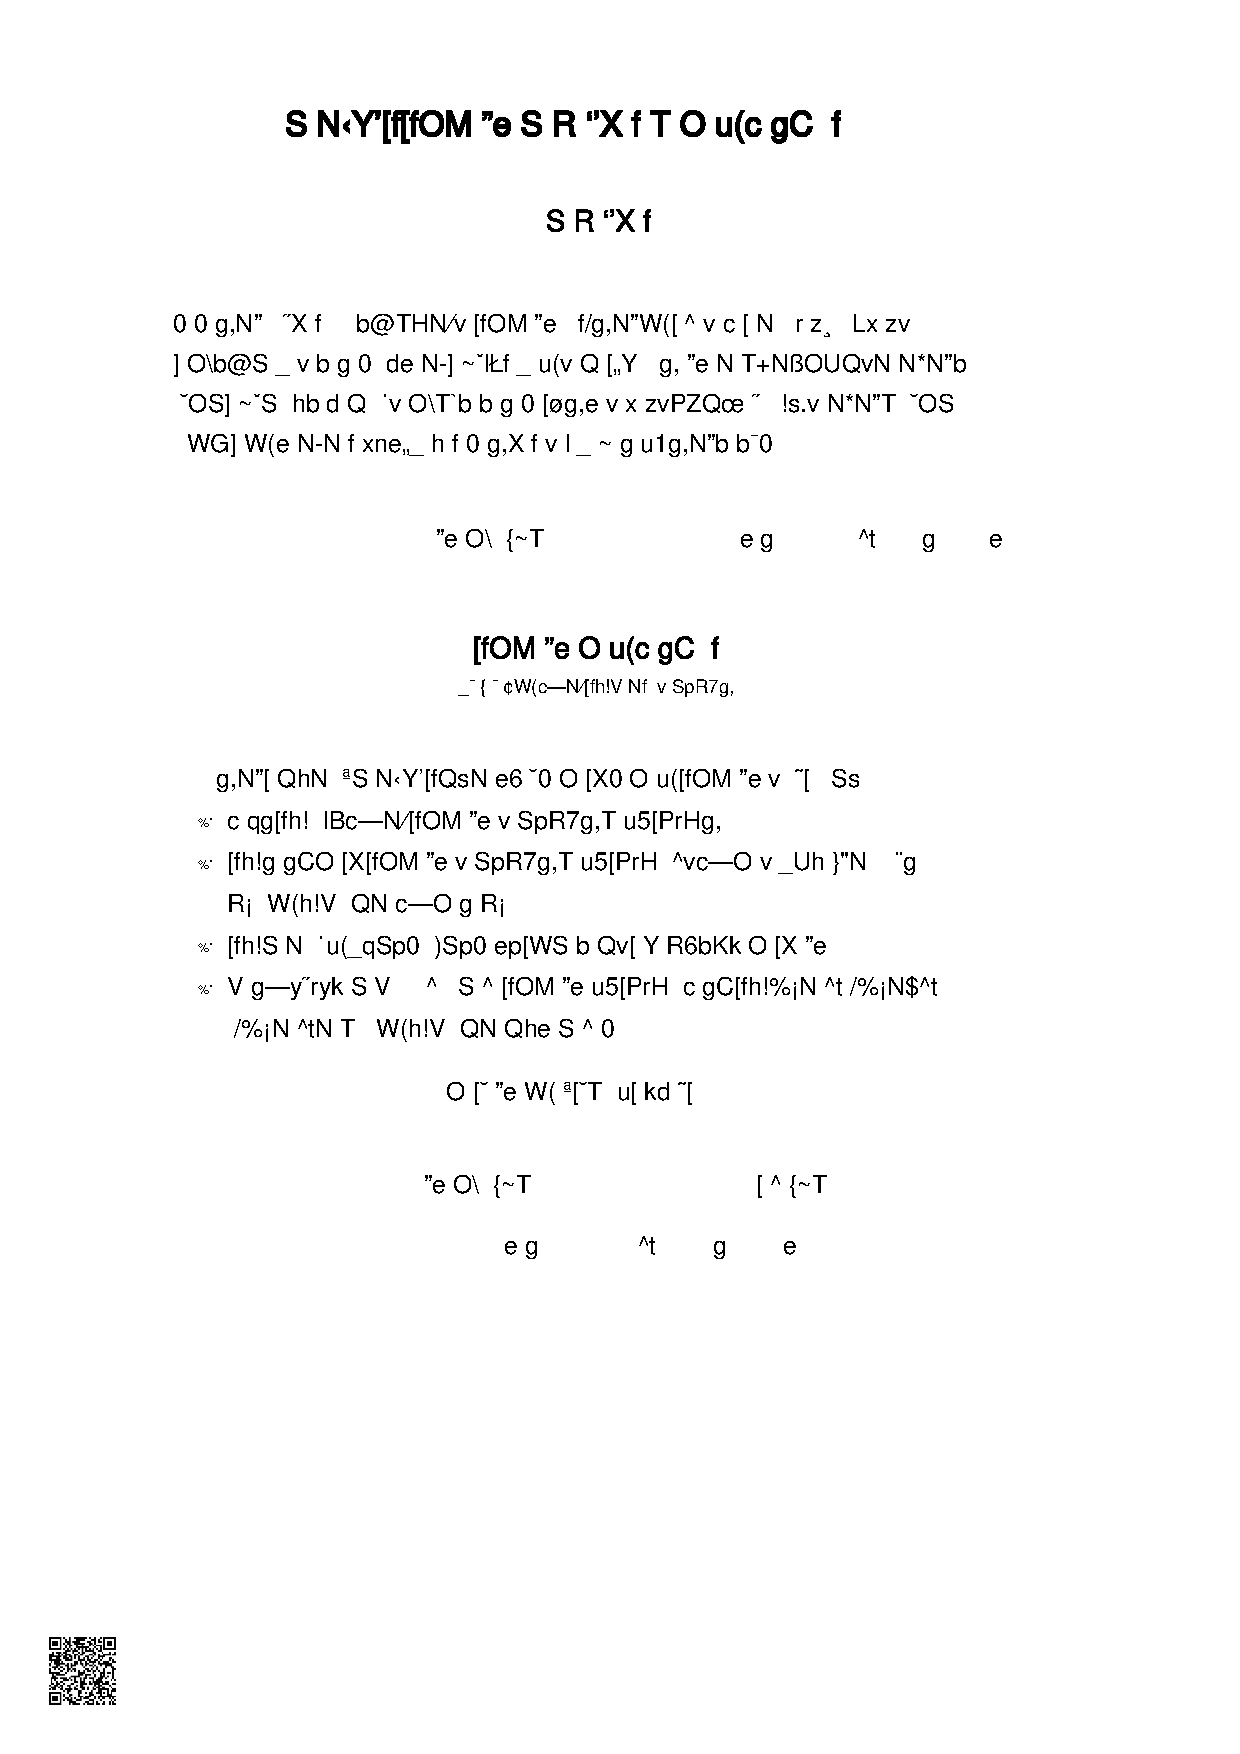
\includegraphics[height = 1.2448\textheight]{img/lwsm_180xxxxxxx.pdf}
		}
	\end{textblock}
}

% vim:ts=4:sw=4

\end{document}

% vim:ts=4:sw=4